% ----------------------------------------------------------------------
%
%
%
%
% ----------------------------------------------------------------------

% ----------------------------------------------------------------------
%                   LATEX TEMPLATE FOR PhD THESIS
% ----------------------------------------------------------------------

% based on Harish Bhanderi's PhD/MPhil template, then Uni Cambridge
% http://www-h.eng.cam.ac.uk/help/tpl/textprocessing/ThesisStyle/
% corrected and extended in 2007 by Jakob Suckale, then MPI-CBG PhD programme
% and made available through OpenWetWare.org - the free biology wiki

%: Style file for Latex
% Most style definitions are in the external file PhDthesisPSnPDF.
% In this template package, it can be found in ./Latex/Classes/
\documentclass[twoside,11pt]{Latex/Classes/PhDthesisPSnPDF}

	
%: Macro file for Latex
% Macros help you summarise frequently repeated Latex commands.
% Here, they are placed in an external file /Latex/Macros/MacroFile1.tex
% An macro that you may use frequently is the figuremacro (see introduction.tex)
\include{Latex/Macros/MacroFile1}


\usepackage[T1]{fontenc}
%\usepackage{pvscript}
\usepackage{amssymb}
\usepackage{amsmath}
\usepackage{epigraph}
\usepackage{amsthm}
\usepackage{amsfonts}
\usepackage[usenames,dvipsnames,svgnames,table]{xcolor}

\usepackage{graphicx}
\usepackage{caption}
\usepackage{subcaption}

\usepackage{mathrsfs}
\usepackage{verbatim}
%\usepackage{therefore}
\usepackage{enumerate}
\usepackage{bm}

\usepackage{float}
\usepackage{wrapfig}
\usepackage{epsfig}
\usepackage{epstopdf}
\epstopdfsetup{outdir=./}
\setcitestyle{square}


\usepackage{csquotes}
%\usepackage[backend=biber,url=true,style=alphabetic]{biblatex}
\PassOptionsToPackage{style=alphabetic}{biblatex}
\usepackage{filecontents}

%\usepackage{embedfile}




% Diagrams
  \usepackage{tikz}
  \usetikzlibrary{matrix,arrows}
  \tikzset{node distance=10em, auto}
  \usetikzlibrary{positioning}
  \usepackage{tikz-cd}



\setlength{\parindent}{0pt}


%\usepackage[italian]{babel}
\setlength{\epigraphwidth}{.6\textwidth}

\usepackage[utf8]{inputenc} %Questo permette di scrivere le lettere accentate
\PassOptionsToPackage{english}{babel}
%\PassOptionsToPackage{0pt}{parident}


%Comandi
  \newcommand{\AND}{\qquad \text{and} \qquad}
  \newcommand{\OR}{\qquad \text{or} \qquad}
  \newcommand{\implica}{\quad \Longrightarrow \quad}
  \newcommand{\st}{\; \text{s.t.} \;}
  \newcommand{\fora}[2]{, \qquad \forall #1 \in #2}
  \newcommand{\set}[1]{\left\{\; #1 \; \right\}}


%Generic commands
  \newcommand{\C}{\mathbb{C}}
  \newcommand{\R}{\mathbb{R}}
  \newcommand{\N}{\mathbb{N}}
  \newcommand{\Q}{\mathbb{Q}}
  \newcommand{\A}{\mathbb{A}}
  \newcommand{\Z}{\mathbb{Z}}

  \newcommand{\PP}{\mathbb{P}}

  \newcommand{\sab}{\sum_{(a)(b)}}
  \newcommand{\e}{\varepsilon}
  \newcommand{\D}[2]{\frac{\partial #1}{\partial #2}}
  \newcommand{\dd}{\partial}
  \newcommand{\al}{\alpha}
  \newcommand{\alb}{{\alpha\beta}}
  \newcommand{\w}{\omega}
  \newcommand{\ph}{\varphi}
  \newcommand{\eps}{\varepsilon}



%Cal letters


  %\newcommand*\calO{\includegraphics{calO}}

  \newcommand{\E}{$\mathcal{E}\;$}
  \newcommand{\F}{$\mathcal{F}\;$}

  \newcommand{\calZ}{\mathcal{Z}}
  \newcommand{\calC}{\mathcal{C}}
  \newcommand{\calO}{\mathcal{O}}
  \newcommand{\calM}{\mathscr{M}}
  \newcommand{\calL}{\mathcal{L}}
  \newcommand{\calN}{\mathcal{N}}
  \newcommand{\calD}{\mathcal{D}}
  \newcommand{\calI}{\mathcal{I}}
  \newcommand{\calT}{\mathcal{T}}

%Frak letters
  \newcommand{\frakm}{\mathfrak{m}}

%Others

  \newcommand{\scr}[1]{\mathscr{#1}}
  \newcommand{\mcal}[1]{\mathcal{#1}}
  \newcommand{\scN}{\mathscr{N}}
  \newcommand{\scD}{\mathscr{D}}
  \newcommand{\scL}{\mathscr{L}}
  \newcommand{\scO}{\mathscr{O}}
  \newcommand{\scI}{\mathscr{I}}
  \newcommand{\LD}{\mathscr{L}(D)}
  \newcommand{\T}{\mathcal{T}}

  \newcommand{\PG}{\PP^{g-1}}


  \newcommand{\OX}{\calO_X}
  \newcommand{\OY}{\calO_Y}
  \newcommand{\OC}{\calO_C}
  \newcommand{\OD}{\calO(D)}
  \newcommand{\OXD}{\OX(D)}
  \newcommand{\ND}{\calN_D}
  \newcommand{\ODD}{\calO_D(D)}

  \newcommand{\wpd}{\widebar{\phi(D)}}


  \newcommand{\into}{\hookrightarrow}
  \newcommand{\tolong}{\longrightarrow}
  \newcommand{\toiso}{\overset{\cong}\longrightarrow}

  \newcommand{\RRo}{Riemann-Roch}
  \newcommand{\RR}{Riemann-Roch }

  \newcommand{\BNo}{Brill-Noether}
  \newcommand{\BN}{Brill-Noether }

  \newcommand{\ses}{short exact sequence }
  \newcommand{\sess}{short exact sequences }
  \newcommand{\les}{long exact sequence }
  \newcommand{\trf}{transition functions }

  \newcommand{\ABiff}{if and only if }


  \newcommand{\IF}{\quad\text{if}\quad}
  \newcommand{\WHEN}{\quad\text{when}\quad}


  \newcommand{\Cech}{\v{C}ech }


  \newcommand{\Mtt}{\tilde{M}_t}  
  \newcommand{\Xdr}{X_d^r}  
  \newcommand{\Xdrr}{ \underline{X}_d^{r} }  
  \newcommand{\Wdr}{W_d^r}  
  \newcommand{\Wdrr}{ \underline{W}_d^{r} }  
  \newcommand{\Gdr}{G_d^{\,r}}  

  \newcommand{\pairing}{\langle\,\bullet,\;\bullet\,\rangle}  
  \newcommand{\pair}[2]{\langle\, #1,\; #2 \,\rangle}  


  \newcommand{\uA}{\underline{A}}

%Sequences
  \newcommand{\SES}[3]{ 0 \to #1 \to #2 \to #3 \to 0 }

  \newcommand{\da}[1]{\left\downarrow{\scriptstyle#1}\vphantom{\displaystyle\sum}\right.}

  \newcommand{\prefive}[5]{%
      \def\tempa{#1}%
      \def\tempb{#2}%
      \def\tempc{#3}%
      \def\tempd{#4}%
      \def\tempe{#5}%
  }
  \newcommand{\five}[5]{%
    \begin{array}{ccccccccccccc}
      0 & \to   & #1        & \to   & #2        & \to   & #3        & \to   & #4        & \to   & #5          & \to & 0 \\\\
        &       & \da{}     &       & \da{}     &       & \da{}     &       & \da{}     &       & \da{}       &     &   \\\\
      0 & \to   & \tempa    & \to   & \tempb    & \to   & \tempc    & \to   & \tempd    & \to   & \tempe      & \to & 0 
    \end{array}  
  }



%Lists
\newcommand{\ABList}[2]{ #1_{1},\dots,#1_{#2} }


\newcommand{\separator}{\par
  \kern20pt % space above the rules
  \hrule height 0.5pt
  \kern1pt % space between the rules
  \hrule height 0.5pt
  \kern20pt % space below the rules
}


% Math Operators
    
  \DeclareMathOperator{\Reg}{Reg}
  \DeclareMathOperator{\Gal}{Gal}
  \DeclareMathOperator{\presheaf}{pre}
  \DeclareMathOperator{\id}{id}
  \DeclareMathOperator{\im}{Im}
  \DeclareMathOperator{\coker}{coker}
  \DeclareMathOperator{\fraction}{Frac}
  \DeclareMathOperator{\homog}{hom}
  \DeclareMathOperator{\Char}{Char}
  \DeclareMathOperator{\Spann}{Span}
  \DeclareMathOperator{\Span}{Span}
  \DeclareMathOperator{\Hom}{Hom_k}
  \DeclareMathOperator{\HomS}{Hom_S}
  \DeclareMathOperator{\rank}{rank}
  \DeclareMathOperator{\Prin}{Prin}
  \DeclareMathOperator{\Set}{Set}
  \DeclareMathOperator{\Exp}{exp}
  \DeclareMathOperator{\Mat}{Mat}
  \DeclareMathOperator{\codim}{codim}
  \DeclareMathOperator{\Res}{Res}
  \DeclareMathOperator{\Supp}{Supp}
  \DeclareMathOperator{\Fitt}{Fitt}
  \DeclareMathOperator{\FittS}{FittS}
  \DeclareMathOperator{\height}{height}
  \DeclareMathOperator{\Grass}{Grass}
  \DeclareMathOperator{\Sym}{Sym}
  \DeclareMathOperator{\Fib}{Fiber}

  \DeclareMathOperator{\Cl}{Cl}
  
  \DeclareMathOperator{\DivB}{\mathbf{Div}}
  \DeclareMathOperator{\PicB}{\mathbf{Pic}}
  
  \DeclareMathOperator{\Div}{Div}
  \DeclareMathOperator{\EDiv}{EDiv}
  \DeclareMathOperator{\Pic}{Pic}
  \newcommand{\Dd}{X_d}
  \newcommand{\Pd}{\Pic^{\,d}_X}
  \newcommand{\Dm}{X_m}
  \newcommand{\Pm}{\Pic^{\,m}_X}  
  \newcommand{\Dn}{X_n}
  \newcommand{\Pn}{\Pic^{\,n}_X}
  \DeclareMathOperator{\FDiv}{\mathbf{FDiv}}
  \DeclareMathOperator{\FPic}{\mathbf{FPic}}

  \newcommand{\Divxk}{\DivB_{X/k}}
  \newcommand{\Picxk}{\PicB_{X/k}}
  \newcommand{\DivXS}{\DivB_{X/S}}
  \newcommand{\PicXS}{\PicB_{X/S}}

  \DeclareMathOperator{\Spec}{Spec}
  \DeclareMathOperator{\Sch}{Sch}
  \DeclareMathOperator{\Ab}{Ab}

  \DeclareMathOperator{\pre}{pre}

%\theoremstyle{definition}


  \newcommand{\modu}{$\Xdr$ and $\Wdr$}
  \newcommand{\moduu}{$\Xdr$ and $\Wdr$ }


  \newcommand{\Ho}{\operatorname{Hom}{}}
  \newcommand{\HH}{\mathscr{H}}

  \newcommand{\HDD} { H^0(D)_D }
  \newcommand{\Tu}  { Tu }
  \newcommand{\TDu} { T_D u }

  \newcommand{\AJ}{Abel-Jacobi}
  \newcommand{\AJJ}{Abel-Jacobi }


\newtheoremstyle{spacytheorem}
  {1.5em} % Space above
  {1.5em} % Space below
  {\itshape} % Body font
  {0em} % Indent amount
  {\bfseries} % Theorem head font
  {.} % Punctuation after theorem head
  {.5em} % Space after theorem head
  {} % Theorem head spec (can be left empty, meaning `normal')
\theoremstyle{spacytheorem}

\newtheorem{prop}{Proposition}[chapter]
\newtheorem{theo}[prop]{Theorem}
\newtheorem{lemm}[prop]{Lemma}
\newtheorem{coro}[prop]{Corollary}

\newtheoremstyle{named}{}{}{\itshape}{}{\bfseries}{.}{.5em}{\thmnote{#3}}
\theoremstyle{named}
\newtheorem*{namedtheo}{Theorem}


\theoremstyle{theorem}
\newtheorem{notation}{Notation}[]

\theoremstyle{theorem}
\newtheorem{assumption}{Assumption}[]

\theoremstyle{definition}
\newtheorem{example}{Example}[]


\theoremstyle{definition}
\newtheorem{defi}[prop]{Definition}

\theoremstyle{definition}
\newtheorem{rema}[prop]{Remark}







% Widebar

  \makeatletter
  \newcommand*\rel@kern[1]{\kern#1\dimexpr\macc@kerna}
  \newcommand*\widebar[1]{%
    \begingroup
    \def\mathaccent##1##2{%
      \rel@kern{0.8}%
      \overline{\rel@kern{-0.8}\macc@nucleus\rel@kern{0.2}}%
      \rel@kern{-0.2}%
    }%
    \macc@depth\@ne
    \let\math@bgroup\@empty \let\math@egroup\macc@set@skewchar
    \mathsurround\z@ \frozen@everymath{\mathgroup\macc@group\relax}%
    \macc@set@skewchar\relax
    \let\mathaccentV\macc@nested@a
    \macc@nested@a\relax111{#1}%
    \endgroup
  }
  \makeatother



%: ----------------------------------------------------------------------
%:                  TITLE PAGE: name, degree,..
% ----------------------------------------------------------------------
% below is to generate the title page with crest and author name

%if output to PDF then put the following in PDF header
\ifpdf  
    \pdfinfo { /Title  (Algebraic Brill-Noether Theory)
               /Creator (Andrea Barbon)
               /Producer (Andrea Barbon)
               /Author (Andrea Barbon)
               /CreationDate (\today)  %format D:YYYYMMDDhhmmss
               /ModDate (\today)
               /Subject (Algebraic Geometry)
               /Keywords (Brill-Noether Theory) }
    \pdfcatalog { /PageMode (/UseOutlines)
                  /OpenAction (fitbh)  }
\fi


\title{Algebraic Brill-Noether Theory}



% ----------------------------------------------------------------------
% The section below defines www links/email for author and institutions
% They will appear on the title page of the PDF and can be clicked
\ifpdf
  \author{\href{mailto:andrea.3arbon@gmail.com}{Andrea Barbon}}
%  \cityofbirth{born in XYZ} % uncomment this if your university requires this
%  % If city of birth is required, also uncomment 2 sections in PhDthesisPSnPDF
%  % Just search for the "city" and you'll find them.
  %\collegeordept{\href{http://www.vu.nl/math/}{Mathematics Department}}
  \university{
    \href{http://www.ru.nl/english/ }{  Radboud University Nijmegen   }\\ 
    \href{http://www.vu.nl/en/      }{  Vrije Universiteit Amsterdam  }\\ 
    \href{http://www.uva.nl/en/     }{  Universiteit Van Amsterdam    }
  }

  % The crest is a graphics file of the logo of your research institution.
  % Place it in ./0_frontmatter/figures and specify the width
  \crest{\includegraphics[width=10cm]{logo_new}}
  
% If you are not creating a PDF then use the following. The default is PDF.
\else
  \author{Andrea Barbon}
  \cityofbirth{born in Venice}
  \collegeordept{Mathematics Department}
  \university{Radboud University Nijmegen, Vrije Universiteit Amsterdam, Universiteit Van Amsterdam}
  \crest{\includegraphics[width=3cm]{logo}}
\fi

\renewcommand{\submittedtext}{Master Degree in}
\degree{Mathematics}
\degreedate{Academic Year 2013-2014}


% ----------------------------------------------------------------------
       
% turn of those nasty overfull and underfull hboxes
\hbadness=10000
\hfuzz=50pt


%: --------------------------------------------------------------
%:                  FRONT MATTER: dedications, abstract,..
% --------------------------------------------------------------

\begin{document}

%\language{english}

% sets line spacing
\renewcommand\baselinestretch{1.2}
\baselineskip=18pt plus1pt
%\setlength{\parident}{0pt}


%\begin{comment}
  
  %: ----------------------- generate cover page ------------------------

  \maketitle  % command to print the title page with above variables


  %: ----------------------- cover page back side ------------------------
  % Your research institution may require reviewer names, etc.
  % This cover back side is required by Dresden Med Fac; uncomment if needed.

  \newpage
  \vspace{30mm}
  Supervisor: B.J.J. Moonen \hspace{45mm} Second reader: R.M.H. de Jeu

  \vspace{20mm}
  Discussion Date: March 2014

  \vspace{20mm}
  Supervisor sign



  %: ----------------------- abstract ------------------------

  % Your institution may have specific regulations if you need an abstract and where it is to be placed in the document. The default here is just after title.

  
% Thesis Abstract -----------------------------------------------------


%\begin{abstractslong}    %uncommenting this line, gives a different abstract heading
\begin{abstracts}         %this creates the heading for the abstract page

	We give an overview of the foundations and the basic results of the classical \BN Theory, dealing with the geometry of the moduli varieties parametrizing effective divisors and linear series on a given curve.\\
	We mainly follow the treatment proposed in the book \emph{Geometry of Algebraic Curves} written by Arbarello, Cornalba, Griffiths and Harris. 
	The classical theory, as presented in the book, was developed during the last century for curves over the complex numbers.\\ 
	Our discussion, instead, avoids the use of any complex-analytic tool and it is completely formulated in terms of modern algebraic geometry. As a result of this more general approach, we are able to generalize two key results of the classical theory -- the Existence and Connectedness Theorems -- to curves over an arbitrary algebraically closed field.\\
	It is important to highlight that the \BN theory heavily relies on homological algebra and, in particular, a crucial role is played by the so called Petri's map, which is in fact a cohomolgical cup-product homomorphism. Hence it seems reasonable to guess that the concepts described in the classical theory are not strictly dependent on complex analysis and, thus, that most of its results can be extended to more general fields.
	\vspace{12em}
	\begin{center}
		\footnotesize{
			The complete LaTex source of this document can be downloaded from the repository \\ 
			\href{https://github.com/AndreaBarbon/Algebraic-Brill-Noether-Theory}{https://github.com/AndreaBarbon/Algebraic-Brill-Noether-Theory}
		}
	\end{center}

\end{abstracts}
%\end{abstractlongs}


% ---------------------------------------------------------------------- 




  % The original template provides and abstractseparate environment, if your institution requires them to be separate. I think it is easier to print the abstract from the complete thesis by restricting printing to the relevant page.
  % \begin{abstractseparate}
  %   
% Thesis Abstract -----------------------------------------------------


%\begin{abstractslong}    %uncommenting this line, gives a different abstract heading
\begin{abstracts}         %this creates the heading for the abstract page

	We give an overview of the foundations and the basic results of the classical \BN Theory, dealing with the geometry of the moduli varieties parametrizing effective divisors and linear series on a given curve.\\
	We mainly follow the treatment proposed in the book \emph{Geometry of Algebraic Curves} written by Arbarello, Cornalba, Griffiths and Harris. 
	The classical theory, as presented in the book, was developed during the last century for curves over the complex numbers.\\ 
	Our discussion, instead, avoids the use of any complex-analytic tool and it is completely formulated in terms of modern algebraic geometry. As a result of this more general approach, we are able to generalize two key results of the classical theory -- the Existence and Connectedness Theorems -- to curves over an arbitrary algebraically closed field.\\
	It is important to highlight that the \BN theory heavily relies on homological algebra and, in particular, a crucial role is played by the so called Petri's map, which is in fact a cohomolgical cup-product homomorphism. Hence it seems reasonable to guess that the concepts described in the classical theory are not strictly dependent on complex analysis and, thus, that most of its results can be extended to more general fields.
	\vspace{12em}
	\begin{center}
		\footnotesize{
			The complete LaTex source of this document can be downloaded from the repository \\ 
			\href{https://github.com/AndreaBarbon/Algebraic-Brill-Noether-Theory}{https://github.com/AndreaBarbon/Algebraic-Brill-Noether-Theory}
		}
	\end{center}

\end{abstracts}
%\end{abstractlongs}


% ---------------------------------------------------------------------- 

  % \end{abstractseparate}


  %: ----------------------- tie in front matter ------------------------

  \frontmatter
  %\include{0_frontmatter/dedication}
  %\include{0_frontmatter/acknowledgement}

%\end{comment}

  %: ----------------------- contents ------------------------
  \renewcommand{\contentsname}{Index}
  \setcounter{secnumdepth}{3} % organisational level that receives a numbers
  \setcounter{tocdepth}{3}    % print table of contents for level 3
  \tableofcontents            % print the table of contents
  % levels are: 0 - chapter, 1 - section, 2 - subsection, 3 - subsection


%: ----------------------- list of figures/tables ------------------------

%\listoffigures	% print list of figures

%\listoftables  % print list of tables


%: ----------------------- glossary ------------------------

% Tie in external source file for definitions: /0_frontmatter/glossary.tex
% Glossary entries can also be defined in the main text. See glossary.tex
%\include{0_frontmatter/glossary} 

%\begin{multicols}{2} % \begin{multicols}{#columns}[header text][space]
%\begin{footnotesize} % scriptsize(7) < footnotesize(8) < small (9) < normal (10)

%\printnomenclature[1.5cm] % [] = distance between entry and description
%\label{nom} % target name for links to glossary

%\end{footnotesize}
%\end{multicols}



%: --------------------------------------------------------------
%:                  MAIN DOCUMENT SECTION
% --------------------------------------------------------------

% the main text starts here with the introduction, 1st chapter,...
\mainmatter

\renewcommand{\chaptername}{} % uncomment to print only "1" not "Chapter 1"


%: ----------------------- subdocuments ------------------------

% Parts of the thesis are included below. Rename the files as required.
% But take care that the paths match. You can also change the order of appearance by moving the include commands.

%
% this file is called up by thesis.tex
% content in this file will be fed into the main document

%: ----------------------- introduction file header -----------------------
\chapter{Introduction}

%: ----------------------- paths to graphics ------------------------

% change according to folder and file names
\ifpdf
    \graphicspath{{figures/}{figures/}{figures/}}
\else
    \graphicspath{{figures/}{figures/}}
\fi

% ----------------------------------------------------------------------
%: ----------------------- introduction content ----------------------- 
% ----------------------------------------------------------------------
%: ----------------------- HELP: latex document organisation
% the commands below help you to subdivide and organise your thesis
%    \chapter{}       = level 1, top level
%    \section{}       = level 2
%    \subsection{}    = level 3
%    \subsubsection{} = level 4
% note that everything after the percentage sign is hidden from output


\nocite{*}

Lorem ipsum dolor sit amet, consectetur adipisicing elit, sed do eiusmod
tempor incididunt ut labore et dolore magna aliqua. Ut enim ad minim veniam,
quis nostrud exercitation ullamco laboris nisi ut aliquip ex ea commodo
consequat. Duis aute irure dolor in reprehenderit in voluptate velit esse
cillum dolore eu fugiat nulla pariatur. Excepteur sint occaecat cupidatat non
proident, sunt in culpa qui officia deserunt mollit anim id est laborum.

Lorem ipsum dolor sit amet, consectetur adipisicing elit, sed do eiusmod
tempor incididunt ut labore et dolore magna aliqua. Ut enim ad minim veniam,
quis nostrud exercitation ullamco laboris nisi ut aliquip ex ea commodo
consequat. Duis aute irure dolor in reprehenderit in voluptate velit esse
cillum dolore eu fugiat nulla pariatur. Excepteur sint occaecat cupidatat non
proident, sunt in culpa qui officia deserunt mollit anim id est laborum.

Lorem ipsum dolor sit amet, consectetur adipisicing elit, sed do eiusmod
tempor incididunt ut labore et dolore magna aliqua. Ut enim ad minim veniam,
quis nostrud exercitation ullamco laboris nisi ut aliquip ex ea commodo
consequat. Duis aute irure dolor in reprehenderit in voluptate velit esse
cillum dolore eu fugiat nulla pariatur. Excepteur sint occaecat cupidatat non
proident, sunt in culpa qui officia deserunt mollit anim id est laborum.

% this file is called up by thesis.tex
% content in this file will be fed into the main document

%: ----------------------- introduction file header -----------------------
\chapter{Preliminaries and geometrical intuition}

%: ----------------------- paths to graphics ------------------------

% change according to folder and file names
\ifpdf
    \graphicspath{{figures/}{figures/}{figures/}}
\else
    \graphicspath{{figures/}{figures/}}
\fi

% ----------------------------------------------------------------------
%: ----------------------- introduction content ----------------------- 
% ----------------------------------------------------------------------
%: ----------------------- HELP: latex document organisation
% the commands below help you to subdivide and organise your thesis
%    \chapter{}       = level 1, top level
%    \section{}       = level 2
%    \subsection{}    = level 3
%    \subsubsection{} = level 4
% note that everything after the percentage sign is hidden from output


\nocite{*}

In this Chapter we introduce some of the ideas which form the foundations of the classical \BN Theory. 
We define the concepts of divisors and line bundles on a curve and, further, the \AJJ map which associates a line bundle to any effective divisor.
Thanks to the Abel's Theorem, this function can be seen as a quotient map and the corresponding equivalence classes are the so called complete linear series, whose behaviour is one of the central themes of the Theory.
Another key ingredient is the famous \RR Theorem which, as we will see, describes the duality between a linear series and its residual one.

All of these concepts are rather abstract, nevertheless we will try to give some insight on their geometrical meaning, by proposing informal interpretations and by taking advantage of some pictures.
We remark that such drawings only represent the real skeleton of the curvem and, therefore, they should not be intended -- in any way -- as precise representations, but just as sketches which may help the reader to build some geometrical intuition.

\section{Divisors and the \AJJ map}

	Let $X$ be a smooth projective curve over an algebraically closed field $k$. Consider the set $\Div_X$ of divisors over $X$ -- i.e. the free abelian group on the points of $X$ -- and denote by $\EDiv_X$ the subset of effective divisors -- i.e. the free monoid on the points of $X$. One can build an intuitive idea of effective divisors by thinking about the finite formal sum $D=\sum_i m_i P_i$ as a \emph{book-keeping device} containing the points of intersection between $X$ and another variety, where the (positive) coefficient $m_i$ of each point $P_i$ measures the multiplicity of the intersection, as Figure \ref{fig:Divisors} shows.

	\begin{figure}[h]
			\centering
			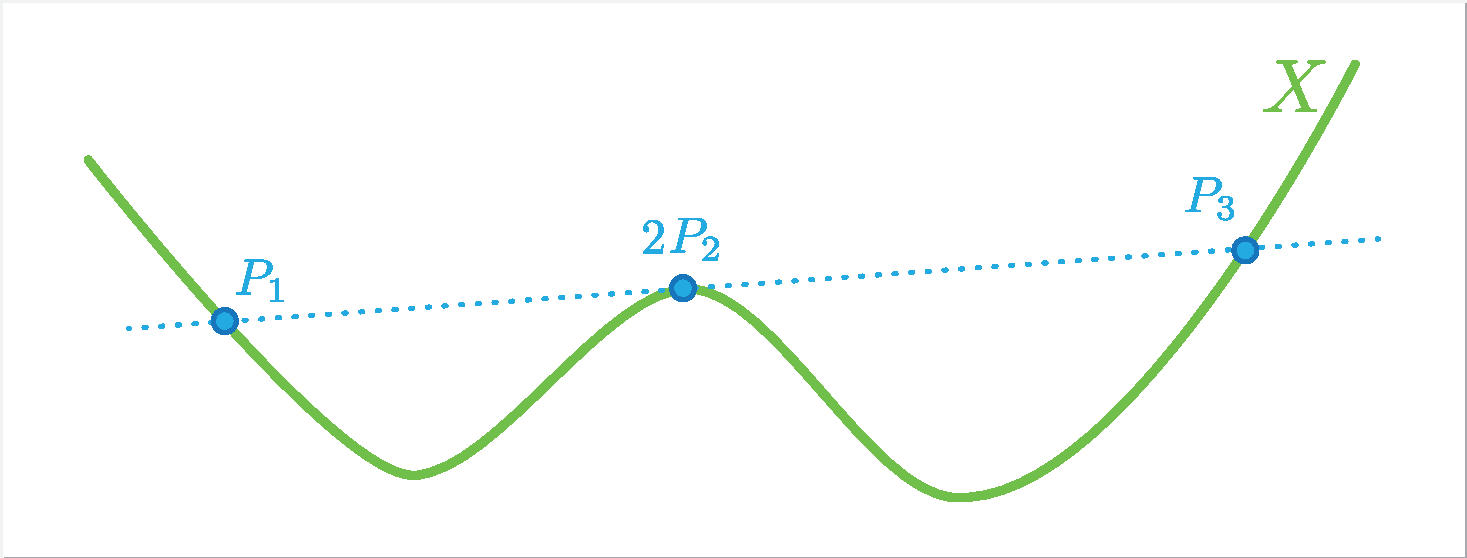
\includegraphics[width=0.9\textwidth]{Divisors.pdf}
			\caption{The effective divisor $P_1 + 2P_2 + P_3$ obtained as the intersection between the curve $X$ and a line}
			\label{fig:Divisors}
	\end{figure}

	Another way to obtain (not necessarily effective) divisors is to start from any non-zero rational map $g$ defined locally on the curve and build a divisor by the recipe
	$$ \Div(g) = (g) = \sum_{P\in X} v_P(g) \cdot P $$
	where $v_P(g)$ is the valuation of $g$ at the point $P$ given by the choice of a local uniformizer. 
	\begin{rema}
		If the divisor of $g$ is given by $(g)=\sum_i m_i P_i$ then, motivated by the definition of \emph{local uniformizer}, we say that on the point $P_i$ the map $g$ presents a \textbf{zero} of order $m_i$ if $m_i>0$, and a \textbf{pole} of order $m_i$ if $m_i<0$.
	\end{rema}	
	Let $f\in k(X)^*$ be globally defined, then the associated divisor $(f)$ is called \textbf{principal divisor} and the well known fact that $\deg(f)=0$ can be explained, informally, by saying that a global rational map on a complete curve has the same number of zeros and poles counted with multiplicity.\\

	The \textbf{degree} of a divisor is defined as the sum of its coefficient, so that it gives a group homomorphism from the set of divisors to $\Z$ and assumes non negative values when restricted to effective divisors. We denote by $\Dd$ the set of effective divisors of degree $d$.\\

	Next, we define the \textbf{Picard group} of $X$ as the sheaf cohomology group
	$$ \Pic_X := H^1(X, \OX^*)\,, $$
	which is well known to be isomorphic to the set of line bundles up to isomorphism, with group structure induced by the usual tensor product of coherent sheaves. 

	To any divisor $D\in \Div_X$ one can associate the line bundle $\OXD$ defined over any open set $U\subset X$ by the prescription
	$$ H^0(U, \OXD) = \left\{\; f \in k(X)^* \mid (f)_{\mid U} + D_{\mid U} \geq 0 \;\right\} $$
	which can be seen as the line bundle whose global sections are locally controlled by $D$. 
	In other words, the sections of $\OXD$ are allowed to present poles on any point of the support of $D$, with order bounded by the coefficient of the point appearing in the formal sum. \\
	It is an easy consequence of the \RR Theorem that every line bundle $L$ on $X$ admits a global section $s$ and, thus, it can be written in the form $L=\OX(D)$ with $D=(s)$ being the divisor corresponding to such a section. Thus we define the \textbf{degree} of $L$ to be the degree of the divisor $D$. We will denote by $\Pd$ the set of line bundles of degree $d$.
	\\
	Based on the above construction, we give a definition of the so called \textbf{\AJJ map} by the assignment
	$$ u: \Div_X\to\Pic_X \qquad D\mapsto \OXD $$ 
	\begin{rema}
		Recall that classically, in the theory of smooth curves over $\C$, the \AJJ map is defined for a one-point divisor $P$ (and then extended linearly) by means of the Abelian integrals as
		$$ u:X_d \to J(X), \qquad P \mapsto \left(\; \int_{P_0}^{P} \omega_1 \;,\; \dots\;,\; \int_{P_0}^{P} \omega_g \;\right) \mod \Lambda, $$
		where $P_0$ is a fixed point of $X$, the $\w_i$'s form a basis of the space of Abelian differentials and $\Lambda$ is a nondegenerate lattice arising from the Riemann bilinear relations.\\
		Our definition of the \AJJ map is simpler, more elegant and does not rely on analytical tools such as path-integration, nevertheless it turns out to be equivalent to its classical counterpart.
	\end{rema}


\section{Linear equivalence and Abel's Theorem}

	Principal divisors can be used to define an equivalence relation on the set of divisors of $X$, by declaring two divisors $D$ and $E$ to be \textbf{linearly equivalent} if they differ by a principal divisor. More precisely, we define
	$$ D\sim E \;\overset{\text{def}}\iff\; \exists\; f \in k(X)^* \text{ such that } E = D + (f) $$
	and, given an effective divisor $D\in \EDiv_X$, we denote by $|D|$ the set of all effective divisors which are linearly equivalent to $D$, the so called \textbf{complete linear series} of $D$.\\
	By sending a global section $f\in H^0(D)$ to the divisor $(f)+D$, we obtain a canonical isomorphism
	$$ \PP H^0(D) \;\cong\; |D| $$
	which identifies the complete linear series of $D$ with the projectification of the vector space of global sections of the line bundle $\OXD$. Motivated by this observation, to any linear subspace $V\subset H^0(D)$ we associate the projective space $\PP V$ and call it a (not necessarily complete) \textbf{linear series}.
	\begin{defi}
		Let $D$ be a divisor of degree $d$ and $V\subset H^0(D)$ a linear subspace of dimension $r+1$. We define a $g_d^r$ to be the linear series associated to $\PP V$.
	\end{defi}

	The classical Abel's Theorem states that the quotient map associated to the equivalence relation defined above is nothing but the \AJJ map or, in other terms, that the fibres of $u$ are complete linear series.
	\begin{namedtheo}[Abel's Theorem]\label{thm:Abel}
		Let $D,E \in \EDiv_X$ be two effective divisors of degree $d$ on $X$. Then
		$$ D\sim E \iff u(D) = u(E). $$
	\end{namedtheo}
	Abel's Theorem was originally proved for Riemann surfaces -- see \cite{GAC} for instance -- but it remains valid for smooth curves over of any algebraically closed field. It plays a crucial role in the \BN theory because it allows to treat linear series as degeneracy loci of the \AJJ map, as we will see in Section \ref{sec:fitt_deg}.
	

\section{The canonical map}

	The recipe we used to obtain divisor $(g)$ from a locally defined rational map $g$ can be extended to the define divisor associated to sections of arbitrary line bundles. In particular, given any global section $\w$ of the cotangent bundle of $X$, we can pick an open cover $\bigcup_i U_i$ of $X$ and a local uniformizer $\pi_i$ for every $U_i$, then $\w$ can be written locally on every $U_i$ as $\w = g_i \; d\,\pi_i$ and the corresponding divisor $(\w) := \sum_i (g_i)$ is called \textbf{canonical divisor}.
	\begin{rema}
		All the canonical divisors on a curve of genus $g$ are linearly equivalent and, as it follows from the \RR Theorem, have degree $2g-2$. Notice that, if $g>0$, a canonical divisor is not principal and its degree is non-zero.
	\end{rema}
	\begin{notation}
		From now on we will abuse notation and write $K$ both for any canonical divisor and for the cotangent bundle $\Omega_X^1$, while the corresponding cohomology groups will be denoted by $H^i(K)$.
	\end{notation}
	
	Next, recall the definition of a base-point-free linear series which we will need for the following construction.
	\begin{defi}
		A $g_d^r$ is said to be \textbf{base-point-free} if there is no point which is contained in the supports of all the divisors belonging to the linear series.
	\end{defi}
	Any base-point-free $g_d^r$ with linear series $\PP V$ can be used to obtain a map of the curve $X$ to a projective space, by considering the assignment
	$$ \phi_V : X\to \PP V^{*} \qquad P\mapsto \set{ s\in V \mid s(P)=0 } \,.$$
	Notice that, since the $g_d^r$ is base-point-free, the requirement $s(P)=0$ gives a non trivial linear condition hence it defines an hyperplane of $V$. Therefore $\phi_V(P)$ can be seen as a point of the dual projective space $\PP V^*$ parametrizing hyperplanes and, thus, $\phi_V$ is a well-defined function.

	\begin{defi}
		We extend the map $\phi_V$ to any effective divisor $D=\sum_{i=1}^d P_i$ with distinct points, by declaring $ \phi_V(D) := \operatorname{span}\{\phi_V(P_1), \dots, \phi_V(P_d)\}$.
	\end{defi}	

	Let us now assume that $X$ has genus $g\geq 2$. Choose any canonical divisor $K$ and recall that the \textbf{genus} of $X$ is defined as $g:=h^0(X, K)$, so that the complete linear series $|K|$ gives rise to a map $\phi_K : X \to \PP^{g-1}$ which is called the \textbf{canonical map}. \\
	It is easy to show that, if $X$ is not hyperelliptic, this map is in fact an embedding and gives a canonical, preferred realization of our curve in a $(g-1)$-dimensional projective space. If the curve is hyperelliptic, instead, $\phi_K:X\to \PP^{g-1}$ is not an embedding, but a $2$ to $1$ map exhibiting $X$ as a double cover of a rational normal curve in $\PP^{g-1}$.
	\begin{figure}[H]
  	\centering
    \begin{subfigure}[b]{0.3\textwidth}
        \centering
					\begin{tikzpicture}[node distance=3.5em, auto]
					\node (X) 									{$X$};
					\node (SP) 	[right of=X]		{$\;$};
				  \node (PP) 	[right of=SP] 	{$\PP^{g-1}$};
				  \node (P1) 	[below of=SP] 	{$\;$};
				  \draw[-stealth, right hook-stealth] 	(X) to node 	{$\phi_K$}				(PP);
				\end{tikzpicture}	  	
      \caption{$X$ not hyperelliptic}
      \label{fig:not_hyp}
    \end{subfigure}
    \qquad
    \begin{subfigure}[b]{0.3\textwidth}
        \centering
					\begin{tikzpicture}[node distance=3.5em, auto]
					\node (X) 									{$X$};
					\node (SP) 	[right of=X]		{$\;$};
				  \node (PP) 	[right of=SP] 	{$\PP^{g-1}$};
				  \node (P1) 	[below of=SP] 	{$\PP^1$};
				  \draw[-stealth] 									(X) to node 	{$\phi_K$}				(PP);
				  \draw[-stealth][swap] 						(X) to node 	{$h$} 					(P1);
				  \draw[right hook-stealth][swap] (P1) to node	{$v_{g-1}$}			(PP);
				\end{tikzpicture}	  	
      \caption{$X$ hyperelliptic}
      \label{fig:hyp}
    \end{subfigure}
	\end{figure}
	
	\begin{assumption}
		For the rest of the Chapter we will assume that $X$ is not hyperelliptic and, for simplicity, we identify $X$ with its isomorphic image $\phi_K(X)$.
	\end{assumption}	

	The most interesting feature of the canonical embedding is that, by construction, any global section of the cotangent bundle $\w\in H^0(X,K)$ corresponds to a hyperplane $H_{\w}\,\subset\,\PP^{g-1}$ which intersects $X$ precisely in the points forming the support of the divisor $(\w)$, counted with the right multiplicity.

	\begin{figure}[h]
		\centering
		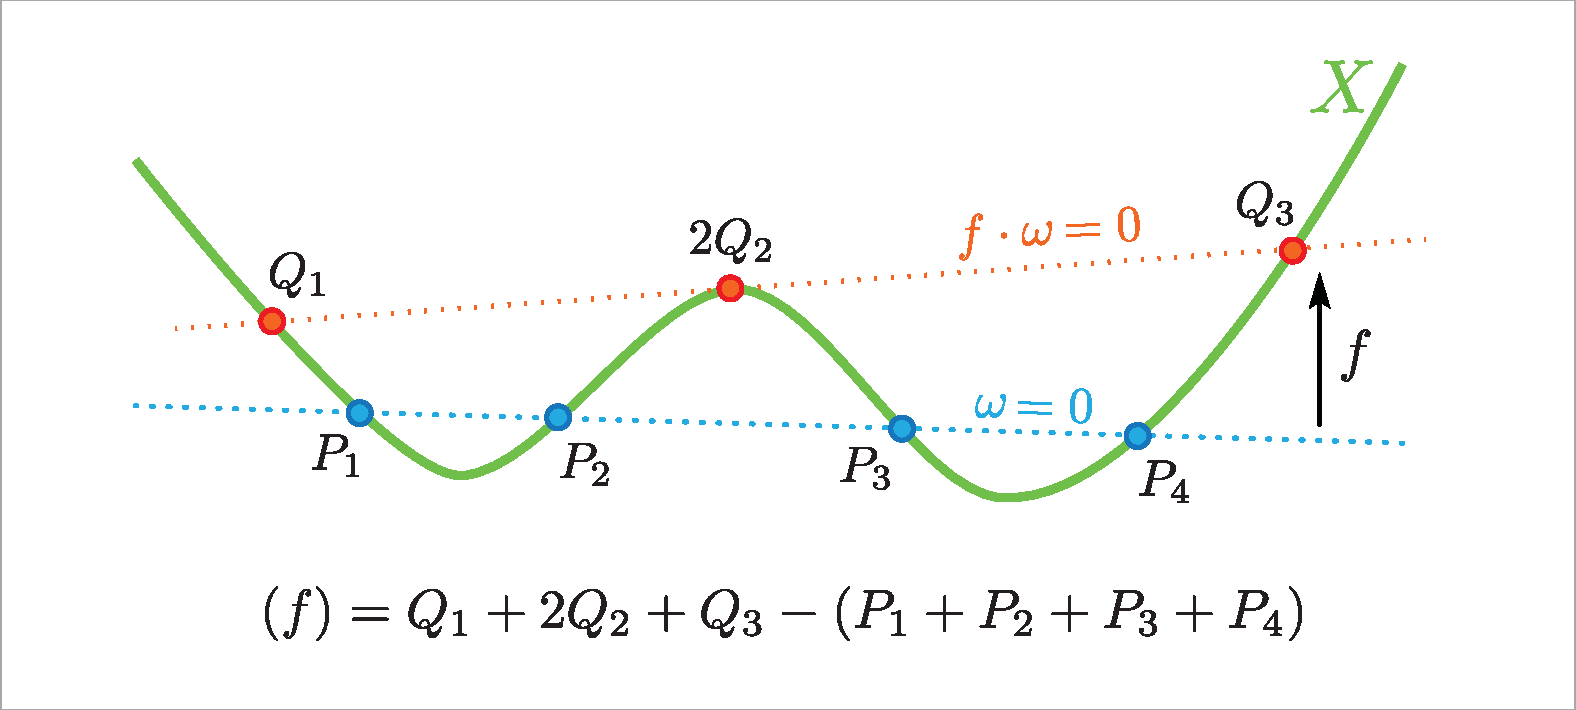
\includegraphics[width=0.9\textwidth]{canonical_embedding_new.pdf}
		\caption{The canonical embedding of a non-hyperelliptic curve of genus $g=3$ in the plane. The picture shows how two canonical divisors are linearly equivalent, being connected by a moving hyperplane }
		\label{fig:canonical_embedding}
	\end{figure}

	Given any rational map $f\in k(X)$, the product $f\cdot \w$ is still an element of $H^0(X,K)$ and, therefore, it corresponds to another hyperplane $H_{f\w}$ via the canonical embedding. Since the support of $(f\cdot\w) = (f)+(\w)$ is in general different from the one of $(\w)$, we can interpret $f$ geometrically as a transformation which \emph{moves} the hyperplane $H_\w$ to a different hyperplane $H_{f\w}$.
	Hence we could informally say that, under the canonical embedding, two divisors are linearly equivalent \ABiff \emph{they are connected by a moving hyperplane}. \\

	This intuitive idea is pictured in Figure \ref{fig:canonical_embedding}, where an non-hyperelliptic curve of genus $g=3$ is considered, so that $\phi_K$ embeds it into $\PP^2$. Notice that, in this example, the linearly equivalent divisors $P_1+P_2+P_3+P_4$ and $Q_1+2Q_2+Q_3$ are both canonical and have degree $2g-2 = 4$.


\section{The \RR Theorem}

	Given any divisor $D$ on $X$, define its \textbf{residual divisor} or \textbf{dual divisor} as $D' := K-D$. Looking at the canonical embedding of our non hyperelliptic curve and considering a divisor $D$ of degree $d<g$ consisting distinct points, we claim that we can always find a canonical divisor $K=(\w)$ such that $D\leq K$. Indeed, we can always find a hyperplane of $\PP^{g-1}$ passing through the $\phi_K(D)$, whose dimension is at most $d-1$.
	In this setting we can think of the support of the residual $D'$ as those points of intersection between the hyperplane and the curve which do not belong to the support of $D$ -- see Figure \ref{fig:Duality}.\\

	\begin{figure}[ht]
			\centering
			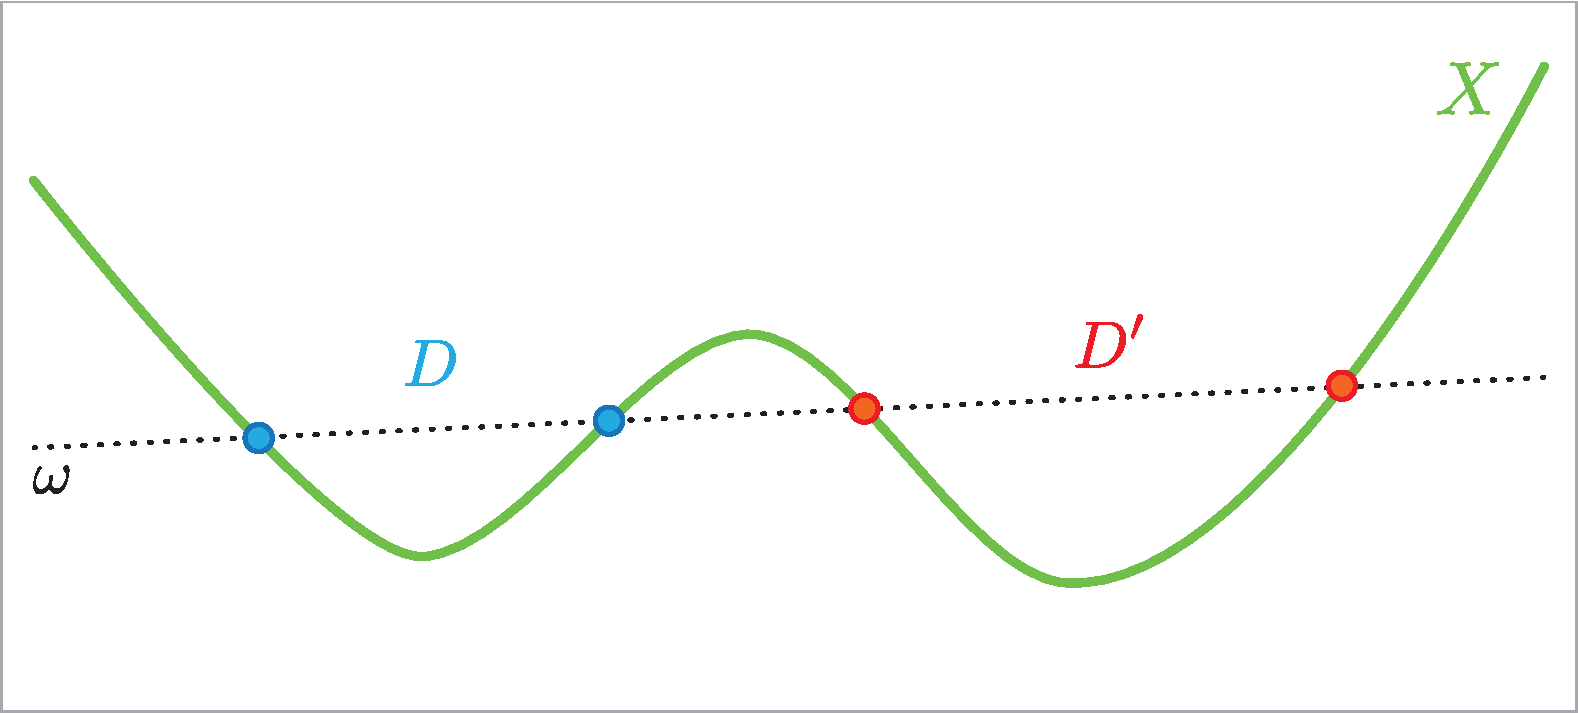
\includegraphics[width=\textwidth]{Duality.pdf}
			\caption{A divisor $D$ of degree $d=2$ and its residual, pictured in the canonical embedding of a genus $3$ curve. In this particular case, since $\deg(\w)=2g-2=4$, the degree $d'$ of the residual divisor is $2$, as well }
			\label{fig:Duality}
	\end{figure}

	The famous \RR Theorem \ref{thm:RR} can be interpreted, thanks to Serre duality, as a statement on the relationship between a divisor and its residual. In fact, given a divisor $D\in \Div_X$ of degree $d$, the \RR formula
	$$ h^0(D) - h^0(D') = d-g+1 $$
	implies that the knowledge of the dimension of $H^0(D)$ is equivalent to that of the dimension of $H^0(D')$ and viceversa.\\

	We highlight, moreover, that the statement of the \RR is completely symmetric with respect to residual duality. Indeed, since the degree of the canonical divisor equals $2g-2$ and the degree of $D'$ is given by $d' = \deg(K)-d$, one can easily see that a completely equivalent formulation of the Theorem is
	$$ h^0(D') - h^0(D) = d'-g+1 $$
	thus showing that the \RR does not discriminate between a divisor and its residual. This implies that the information we can get from the behaviour of a given divisor can be equivalently obtained by looking at its residual and viceversa, a fact which will be exploited to draw Figure \ref{fig:Exceptional_Divisors}.\\

	The relationship between the Theorem and linear series is therefore well understood by means of the above mentioned canonical isomorphism
	$ \PP H^0(D) \;\cong\; |D| $
	which identifies the complete linear series of $D$ with the projectification of the space of global sections of $\OXD$. Therefore, using the standard notation $r(D):= \dim|D| $ for the dimension of $|D|$, we can rewrite the \RR formula as
	\begin{equation}\label{eq:RR}
		r(D') - r(D) = d'-g+1
	\end{equation}
	thus making it clear that it can be interpreted as a statement on the \emph{dimension spread} between a linear series and its residual.\\

	The \RR Theorem is an extremely useful result, with applications ranging from pure mathematics to applied graph theory and even communication engineering. But what is the geometrical meaning of the Riemann-Roch formula? We will try to answer this fascinating question in the following Sections.
	

\section{Special exceptional divisors}\label{sec:special}

	Some divisors on the curve $X$ -- and the corresponding linear series -- are \emph{more important} than others, in the sense that they contain more information about the curve itself.\\ 
	A good reason to study the so called \textbf{special exceptional divisors} of a given curve, as we will exemplify in Section \ref{sec:examples}, is that the behaviour of the corresponding linear series may help distinguish the curve among other curves.\\
	Put $r=r(D)$. For a curve of genus $g$ the region of special exceptional divisors is given, as a subset of the $(d,r)$-plane, by the inequalities
	$$ r>0 \AND 2r<d<g $$ 
	as we picture in Figure \ref{fig:Exceptional_Divisors}. The reasons for these constraints are the following:
	\begin{itemize}
		\item If $r=0$ then the linear series $|D|$ is trivial;
		\item Due to the duality involved in the \RR formula, we can restrict our attention to linear series of degree $d<g$;
		\item For non trivial linear series of degree $d<g$, Clifford's Theorem \ref{thm:Clifford} gives the upper bound $r<d/2$.
	\end{itemize}

	\begin{figure}[ht]
		\centering
		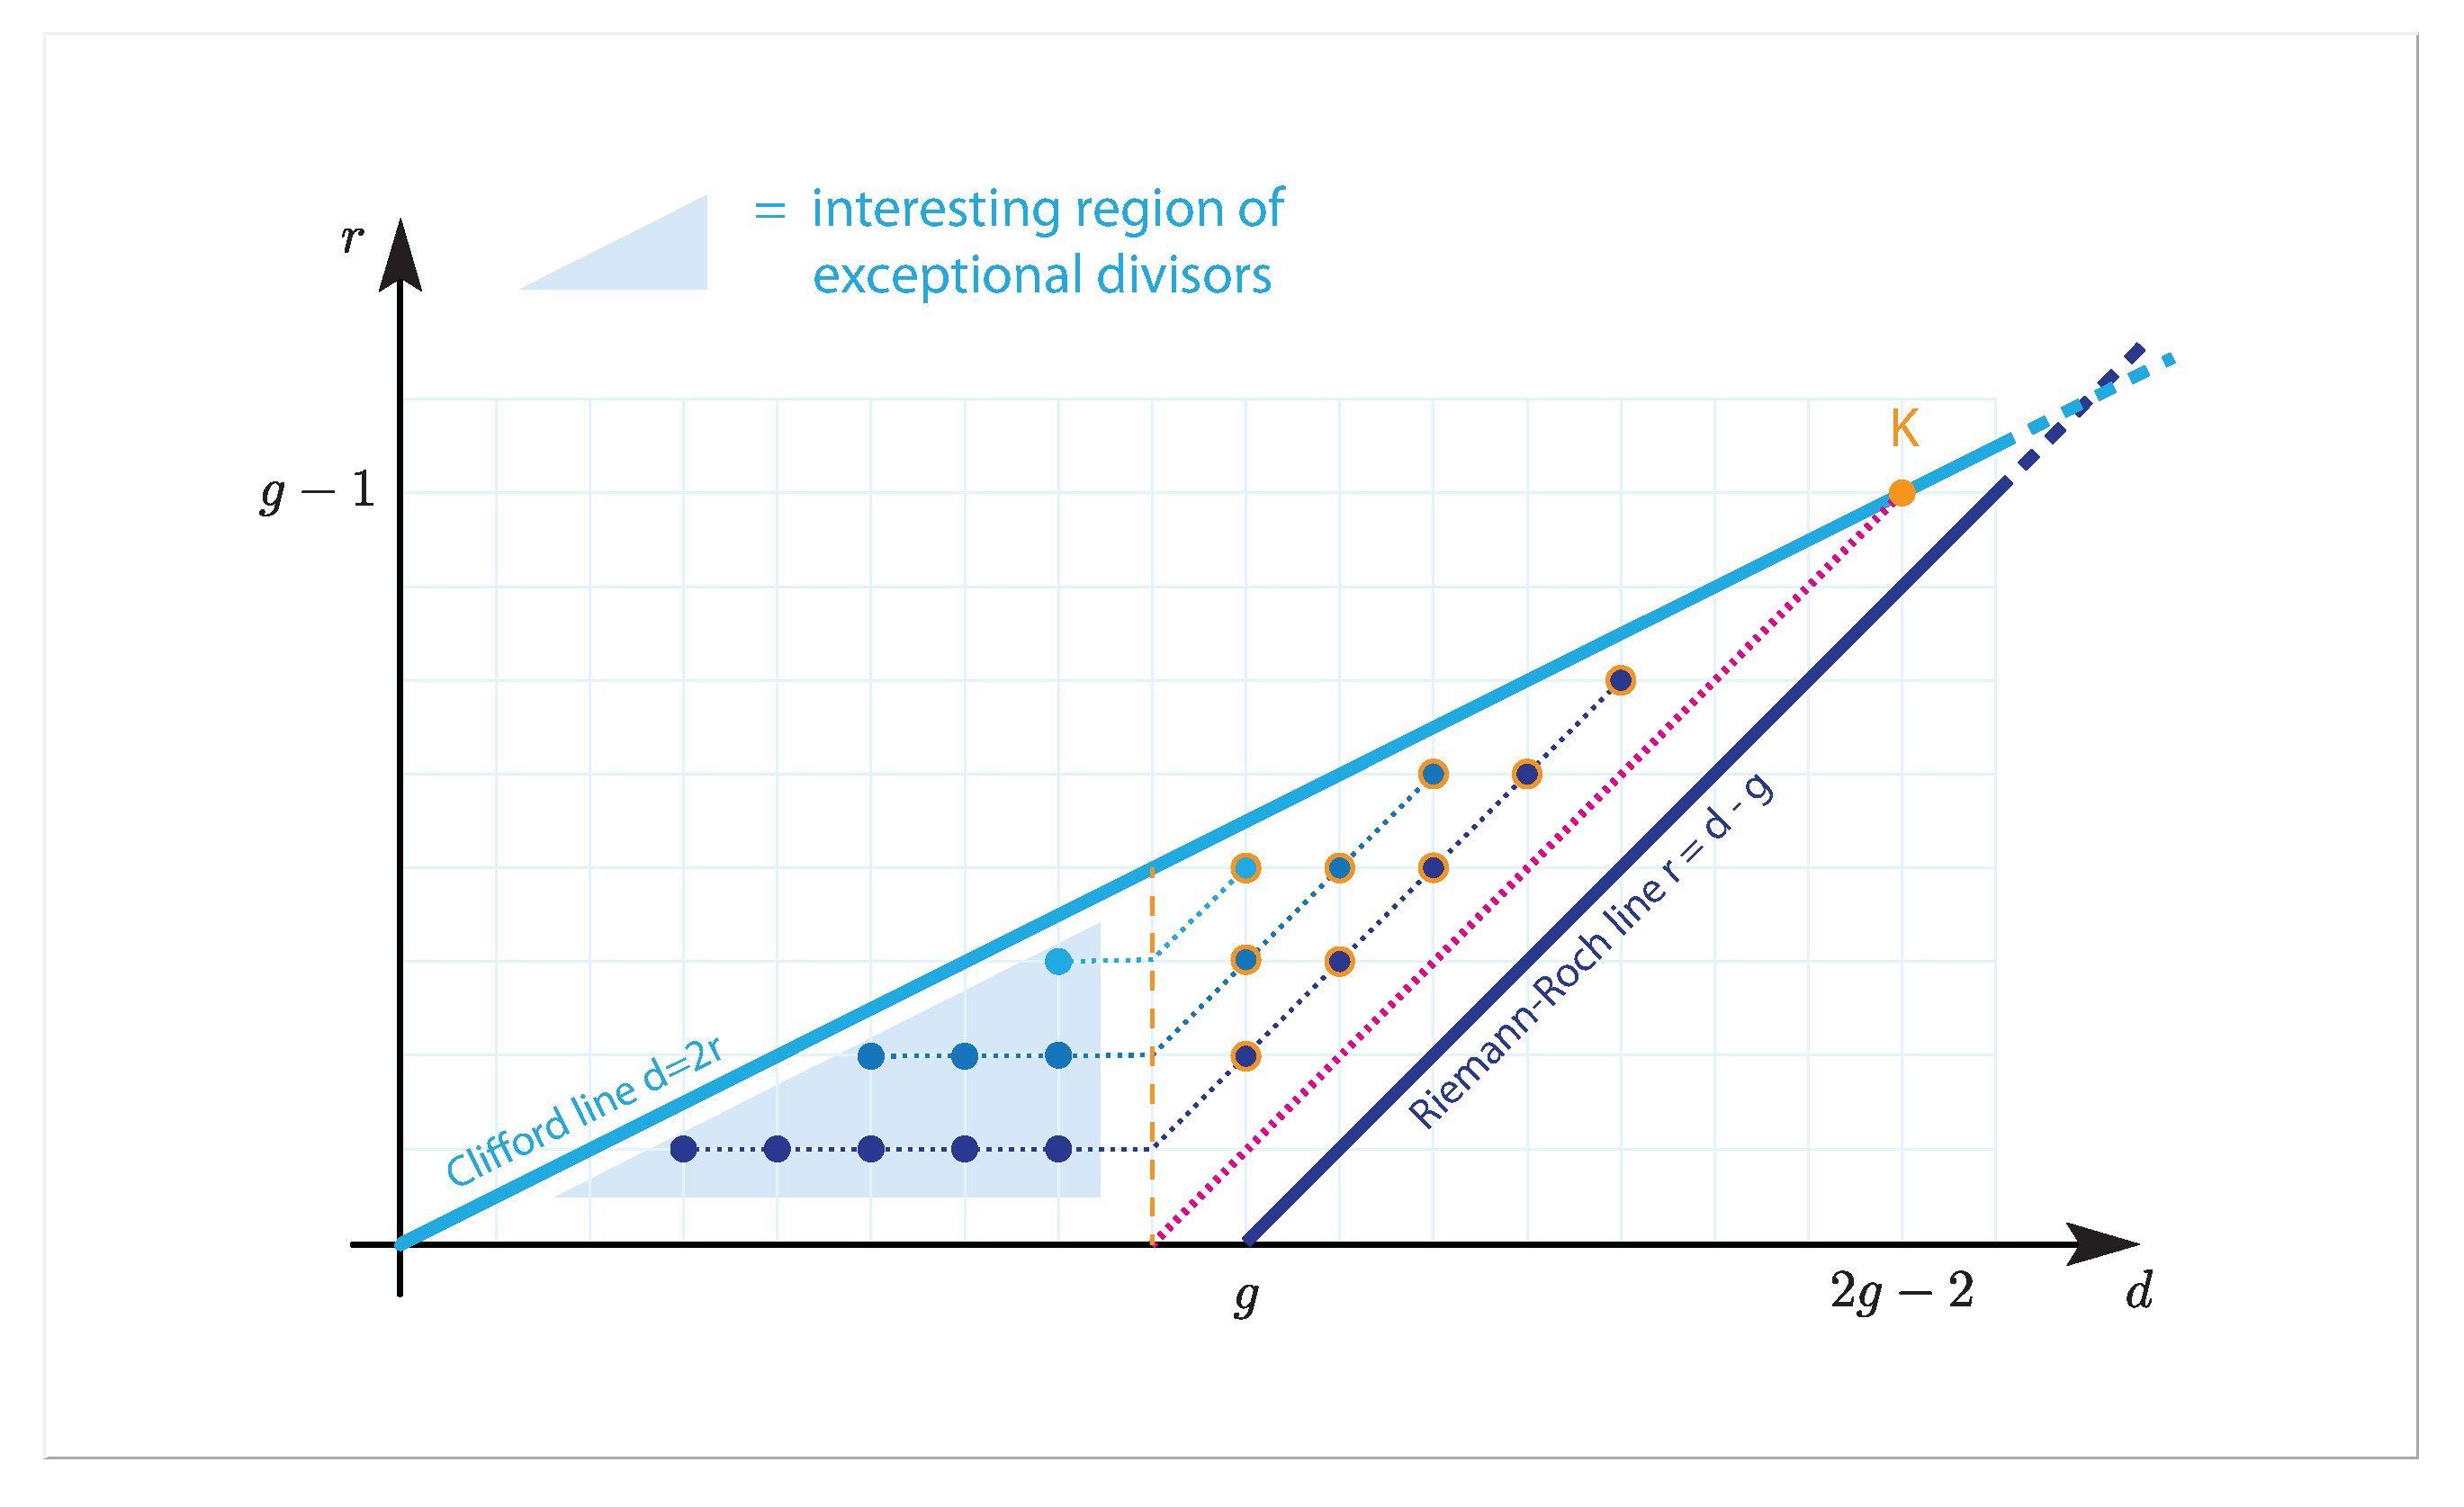
\includegraphics[width=0.85\textwidth]{Exceptional_Divisors_new.pdf}
		\caption{ The region of Special Exceptional divisors for a curve of genus $g=9$ }
		\label{fig:Exceptional_Divisors}
	\end{figure}


\section{Geometrical interpretation}

	In the following we will give some insights into the geometrical meaning of the \RR formula. In order to do so, we start by introducing the cup-product map
	$$ \mu_0: H^0(D)\otimes H^0(K-D) \tolong H^0(K) $$ 
	which is also know as the \textbf{Petri's map} and, as we will see in Chapter \ref{chap:moduli}, plays a fundamental role in the linear approximation of the varieties \moduu parametrizing linear series.\\

	Consider an effective divisor $D$ of degree $d<g$ consisting of distinct points and notice that the vector space $H^0(K-D)$ can be interpreted as the linear subspace consisting of those $\w\in H^0(K)$ such that $(\w)\geq K$ or, in other words, $\PP H^0(K-D)$ parametrizes the hyperplanes of $\PP^{g-1}$ which cut $X$ in a set of points containing $D$. Among these hyperplanes there is a unique one passing through the support of the residual $D'$, which can be identified with the unique generator of $H^0(K-D-D')\cong H^0(\OX)$.\\ 
	Now, by restricting the Petri's map to $H^0(D)\otimes H^0(K-D-D')$, we get a map
	$$ \mu_0: H^0(D)\otimes H^0(K-D-D') \tolong H^0(K-D') $$
	whose target space corresponds (up to scalar multiplication) to the hyperplanes cutting the curve in a set of points containing the support of $D'$. From the natural isomorphism $H^0(K-D')\cong H^0(D)$ we deduce that the number of such hyperplanes is given by the integer $r(D) = \dim \PP H^0(D)$, a fact which can be used to shade light on the geometrical interpretation of the \RR. Indeed, one can equivalently rewrite the formula \eqref{eq:RR} as
	$$ r(D) = [\;g-1\;] \; - \; [\;d'-r(D')\;] $$
	and observe that $g-1$ is nothing but the dimension of the projective space $\PP^{g-1}$ in which $X$ is canonically embedded. Therefore we see that $d'-r(D')$ equals the number of linearly independent points of the support of $D'$ and, consequently, that the integer $r(D')$ counts the number of independent linear relations among these points. Hence the \RR is \emph{simply} telling us that the complete linear series $|D|$ can be geometrically visualized as a family of hyperplanes passing through $\phi_K(D')$, each one of them cutting $X$ in a set of points consisting of $D'$ plus a divisor in $|D|$.

	Therefore we understand how the fact that the \emph{dimension spread} $r(D)-r(D')$ is a constant depending on $d$ and $g$ has a clear geometrical meaning: a higher number $r(D')$ of independent linear relations among the support of $D'$ corresponds to a larger family of hyperplanes passing through $\phi_K(D')$, the dimension of this family being precisely the dimension $r(D)$ of the linear series $|D|$.\\  

	In the next page, we show two pictures that might help the reader visualizing the geometrical meaning of $r(D)$, in the context of the canonical embedding of a curve of genus $4$. Figure \ref{fig:Example} presents an example of a $g_1^3$, whit one linear relation among the $3$ points of $D$, while Figure \ref{fig:Example2} shows a trivial linear series, where no linear relations among the points of $D$ is present.\\

	Moreover, notice that the above geometrical interpretation allows to exclude some otherwise possible scenarios. For instance, the canonical embedding of a genus $4$ curve cannot appear as pictured in Figure \ref{fig:Impossible}, because this would correspond to the values $d=2$, $d'=4$ and $r(D)=0$, $r(D')=2$ which do not satisfy the \RR formula.
	\vspace{1.5em}
	\begin{figure}[H]
		\centering
		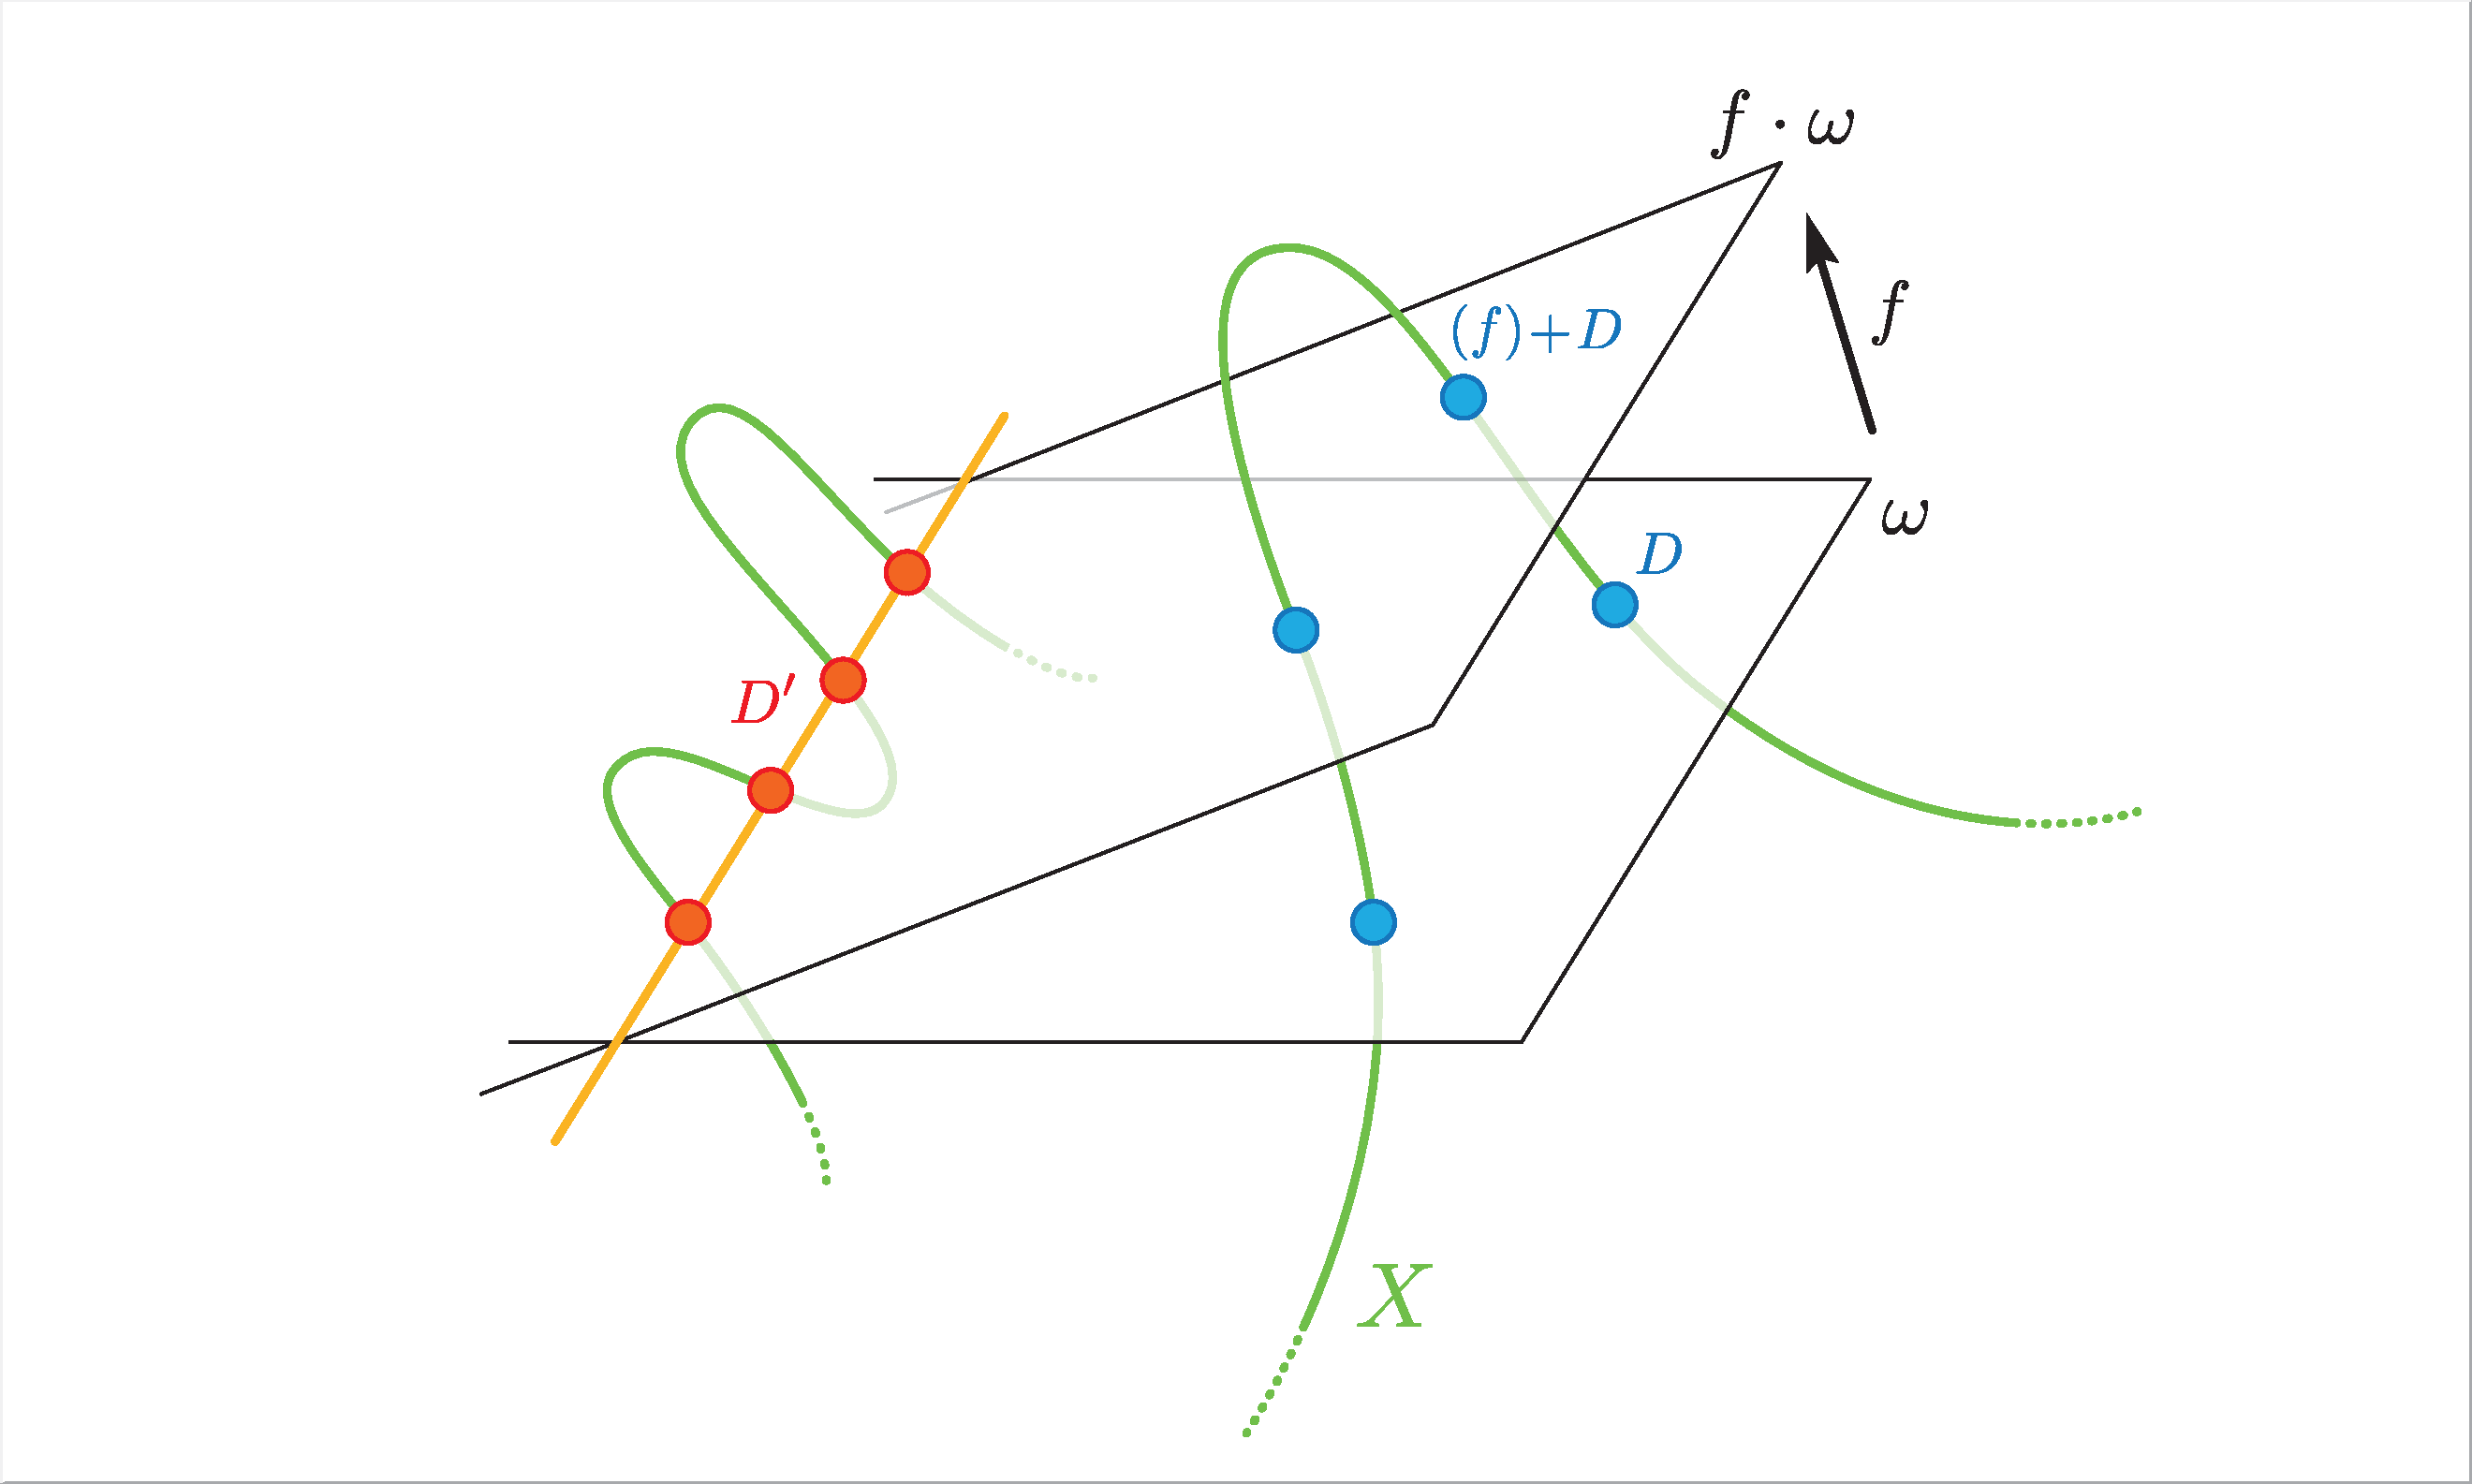
\includegraphics[width=0.85\textwidth]{Impossible.pdf}
		\caption{An hypothetical curve of genus $4$ embedded in $\PP^3$, showing a $g_2^0$ whose residual series is a $g_4^2$. This situation is actually impossible, as one can deduce form the \RR Theorem }
		\label{fig:Impossible}
	\end{figure}

	%in the context of the canonical embedding of a curve of genus $4$\newpage

	\begin{figure}[H]
		\centering
		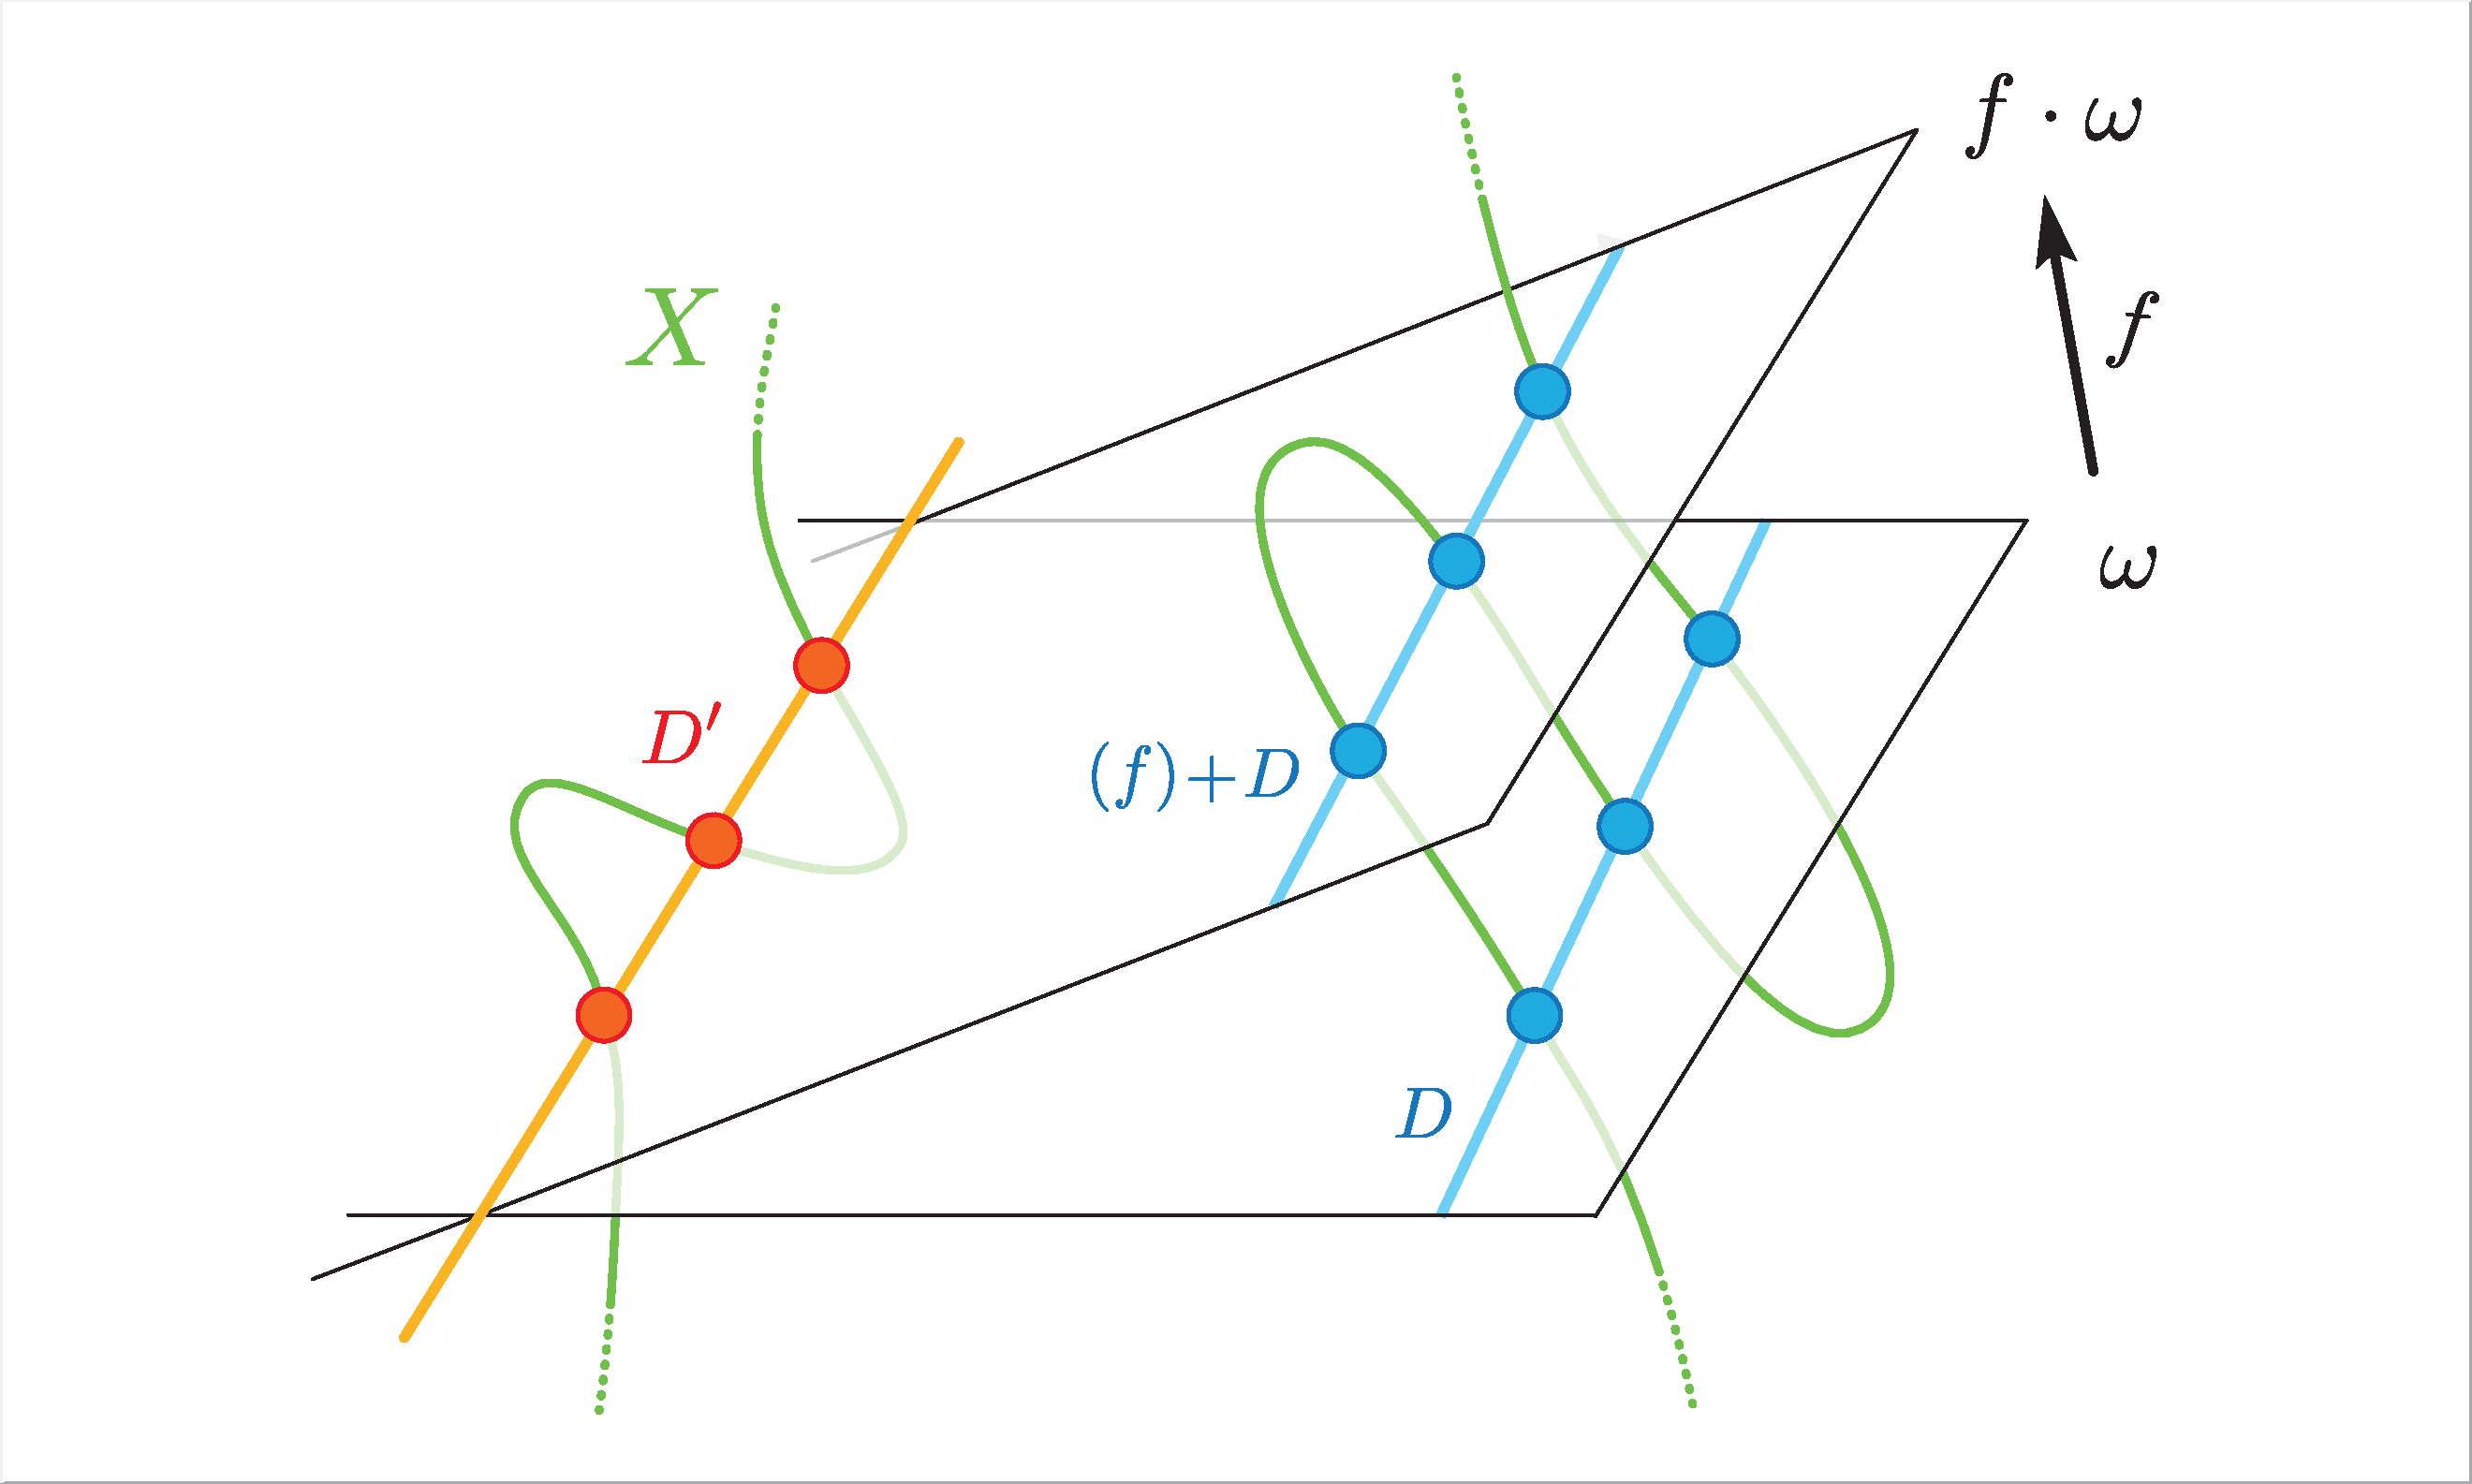
\includegraphics[width=0.85\textwidth]{Example.pdf}
		\caption{An example of a complete linear series on a curve of genus $4$ canonically embedded into $\PP^3$. The global section $f\in H^0(D)$ has poles only on the points of $D$, hence the hyperplane $H_{\w}$ associated to $\w \in H^0(K-D-D')$ is moved away from $D$ by $f$, but stays on the points of the residual divisor $D'$. Notice that, for this particular choice of $D$, there is one linear relation among the points of both $D$ and $D'$, so that $r(D)=r(D')=1$ and each divisor gives rise to a $g_3^1$. }
		\label{fig:Example}
		
		\vspace{4em}

		\centering
		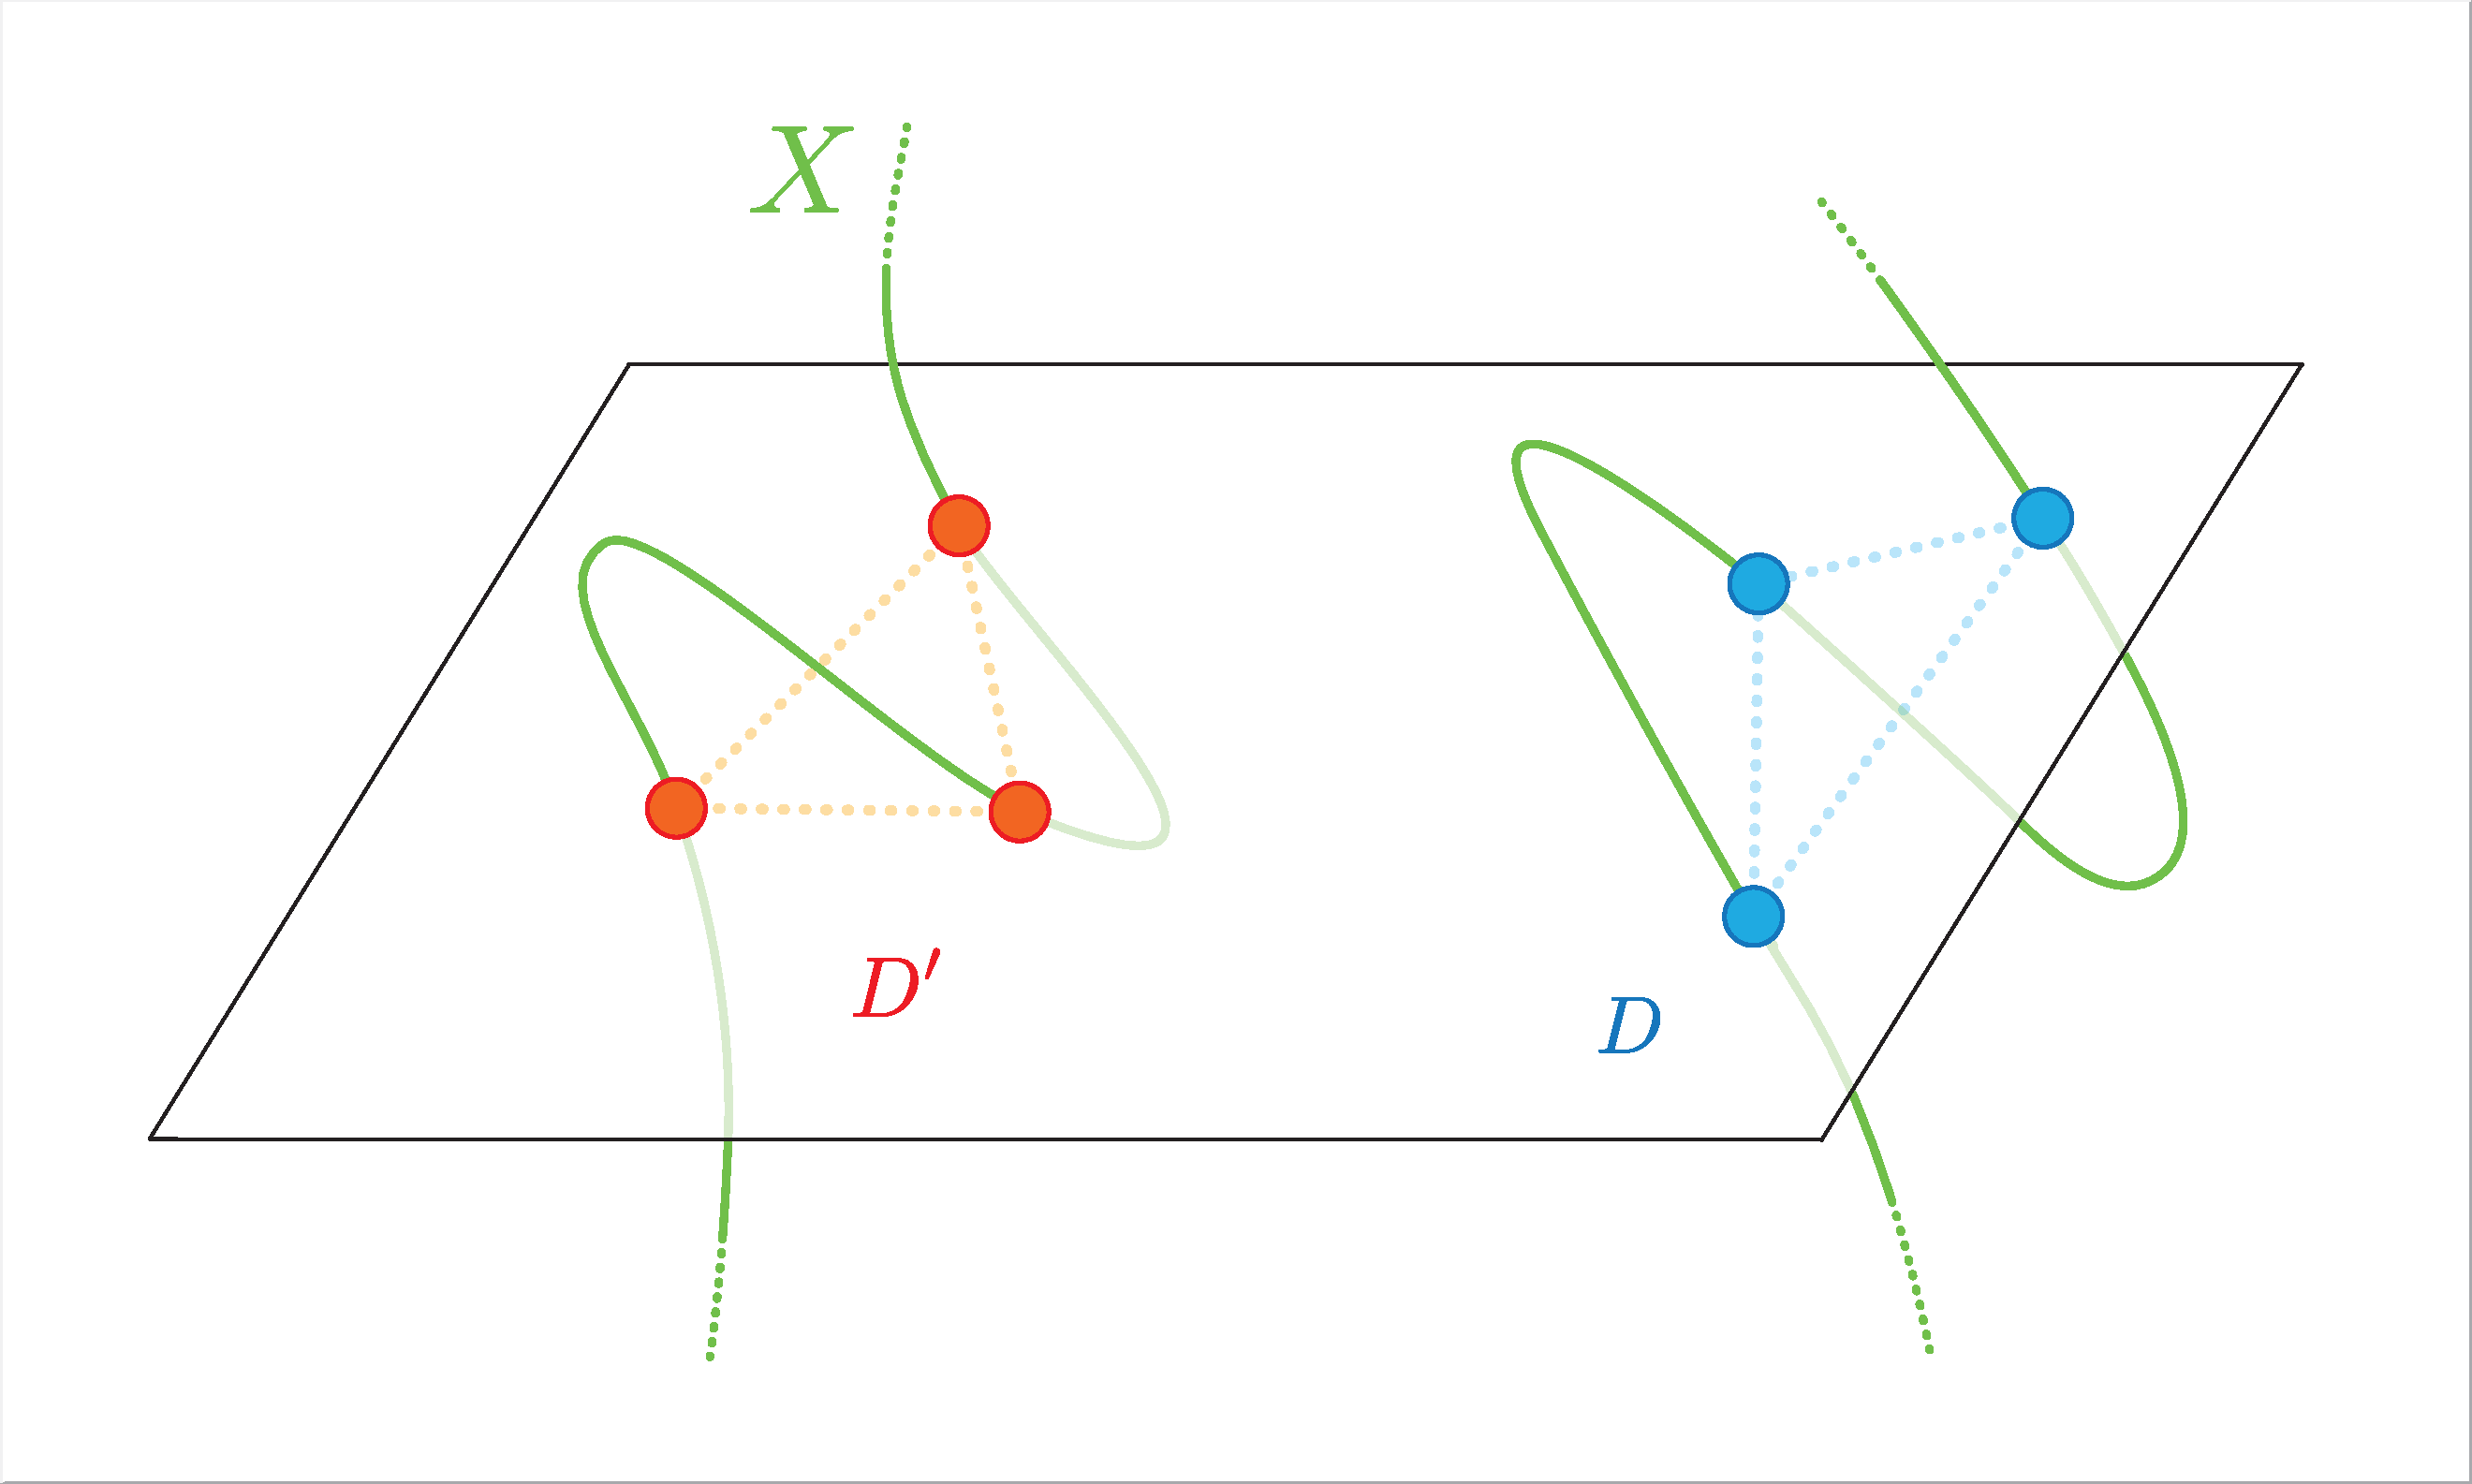
\includegraphics[width=0.85\textwidth]{Example2.pdf}
		\caption{In this example a divisor $D$ of degree $3$ gives rise to a trivial linear series. The reason is that the points of $D'$ are linearly independent, therefore there is only one hyperplane passing through $\phi_K(D+D')$. }
		\label{fig:Example2}
	\end{figure}


\section{Examples}\label{sec:examples}
	
	In this Section we will analyse the case of a non-hyperelliptic curve $X$ of genus $4$ in which, as it follows from the discussion of Section \ref{sec:special}, the only special exceptional linear series -- if any exists -- are $g_1^3$.  
	Actually, the Existence Theorem \ref{thm:existence} states that whenever the \textbf{Brill-Noether number}
	$$ \rho(g,d,r) := g - (r+1)(g-d+r) $$
	is non-negative, then there exists at least one $g_d^r$ on the curve. In our case we find $\rho(4,3,1)=0$ and, as a consequence we deduce that our curve admits a $g_3^1$.\\
	It is a well known fact in algebraic geometry that any smooth projective curve of genus $4$ comes as the complete intersection of a quadric surface with a cubic surface inside $\PP^3$ and, moreover, that any quadric of $\PP^3$ is ( up to projective equivalence ) a ruled surface. Hence we see that there are two distinct possibilities:
	\begin{enumerate}[i)]
		\item If the quadric is smooth, then it is a saddle surface, doubly-ruled by two families of perpendicular lines;
		%In this case there are $2$ distinct $g_3^1$ : one of them cuts on the curve divisors lying on one family of the ruling lines, while the other one  cuts divisors sitting on the perpendicular family -- See Figure \ref{fig:Pringles}
		%
		\item If the quadric is singular, then it is a conic surface and there is only one family of ruling lines, all passing through the singular point. 
		%In this case there is one unique $g_3^1$, and every divisor cut on the curve by the linear series lies on a ruling line passing through the singular point of the quadric -- See Figure \ref{fig:Cone}
 	\end{enumerate}
 	Let us start by looking at the first case of a curve on a smooth quadric surface.

 	\begin{example}\label{ex:smooth_quadric}

 		\begin{figure}[h]
			\centering
			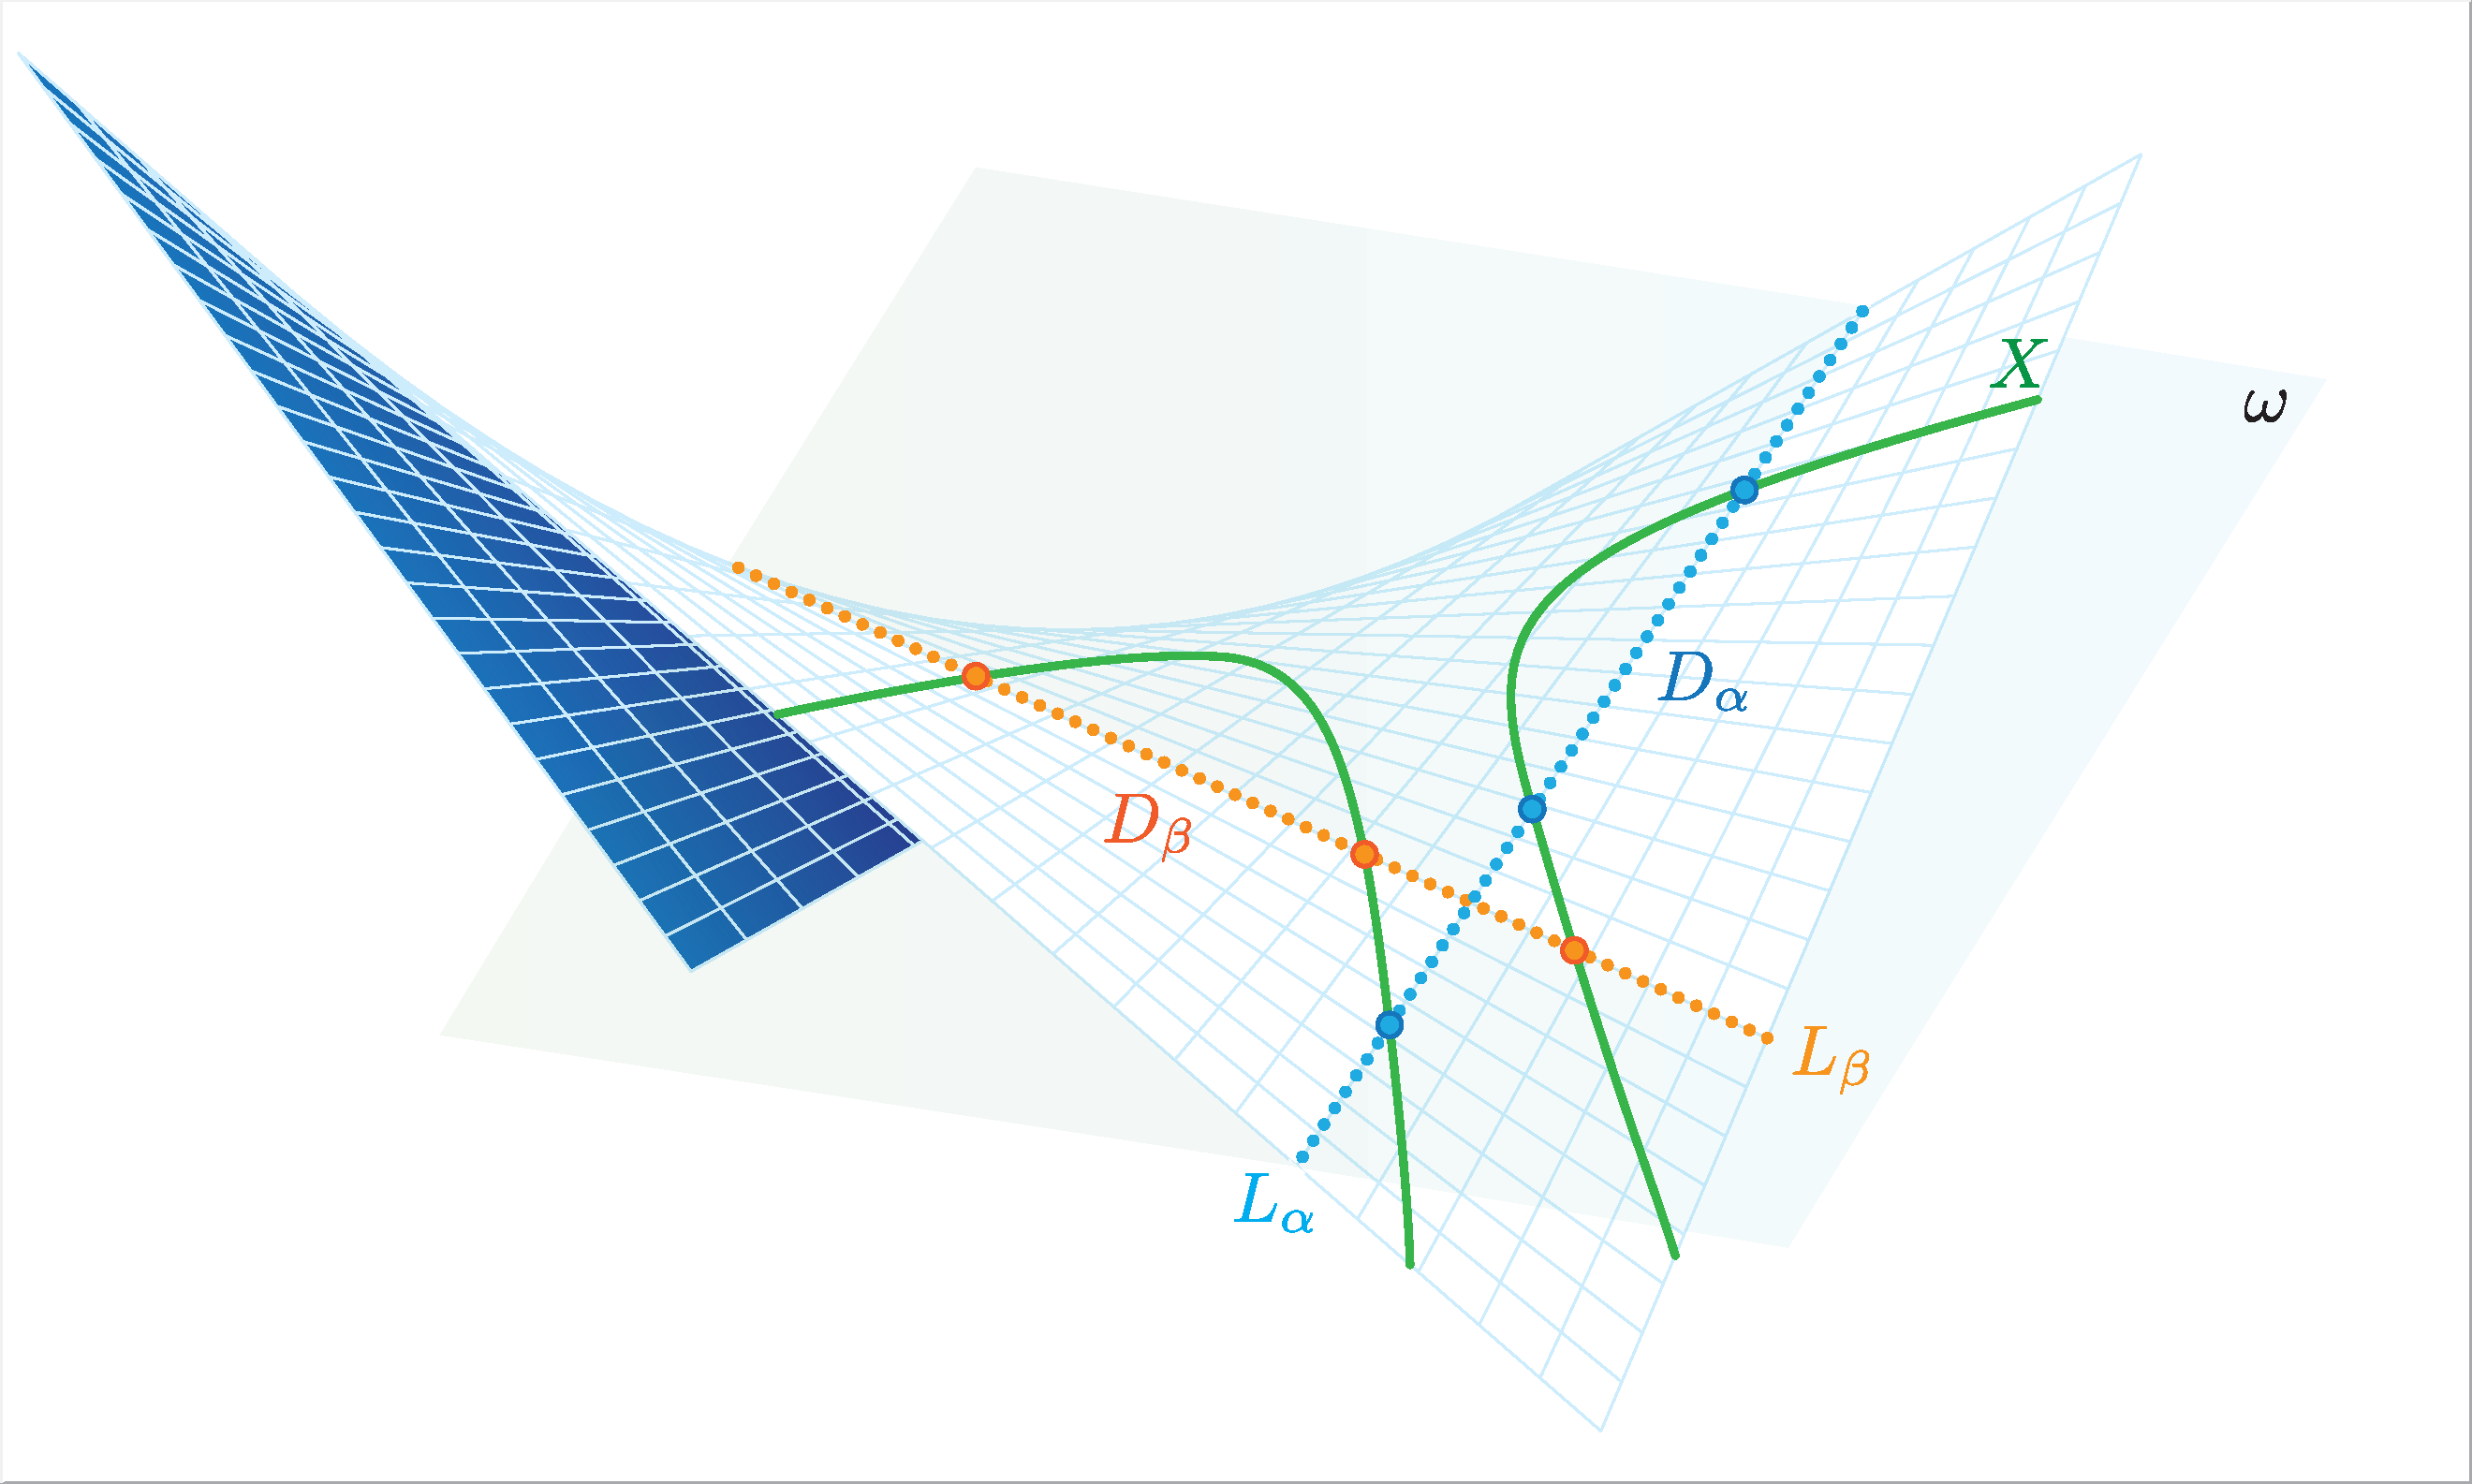
\includegraphics[width=0.85\textwidth]{Pringles2.pdf}
			\caption{ A genus $4$ curve contained in a doubly-ruled smooth quadratic surface -- a hyperbolic paraboloid. The blue dots form the support of a divisor $D_\al$ contained in a $g_3^1$, while the orange ones form the support of the residual $D_\beta$ belonging to the other $g_3^1$ }
			\label{fig:Pringles}
			%\vspace{1em}
		\end{figure}

 		Up to projective equivalence, the smooth quadratic surface $Q$ corresponds to the equation
 		$$ X_0 X_3 = X_1 X_3 $$
 		and it is naturally isomorphic to the product $\PP^1 \times \PP^1$ of two projective lines. The double ruling of $Q$ is given by two $\PP^1$ families of lines
 		$$ A= \begin{cases} X_0=a X_1 \\ X_2=a X_3 \end{cases} \AND B= \begin{cases} X_0=b X_2 \\ X_1=b X_3 \end{cases} $$
 		where the parameters $a$ and $b$ vary in $\PP^1$. It is easy to check that any two lines $L_\al \in A$ and $L_\beta \in B$ intersect in the unique point $[\alb, \beta, \al, 1]$ and, hence, their span is a plane $H_\alb = \Span(L_\al, L_\beta)$. Suppose that such a plane cuts $X$ on the effective divisor
 		$$ H_\alb \cdot X = D_\al + D_\beta, \qquad D_\al\in L_\al, \; D_\beta\in L_\beta $$
 		and recall that, since $H_\alb$ is a hyperplane of $\PP^3$, the divisor $D_\al + D_\beta$ is canonical of degree $2g-2=6$.
 		Each line $L_\al$ and $L_\beta$ moves in a $\PP^1$-family, so it follows that
 		$$ r(D_\al) \geq 1 \AND r(D_\beta) \geq 1 $$
 		and, as a consequence, Clifford's Theorem $\ref{thm:Clifford}$ implies that both $\deg(D_\al)\geq 2$ and $\deg(D_\beta)\geq 2$. But, since $X$ is not hyperelliptic, these inequalities are actually strict and from $\deg(D_\al+D_\beta)=6$ we deduce
 		$ \deg(D_\al) = \deg(D_\beta) = 3 $,
 		thus another application of the Clifford's Theorem ensures that
 		$$ r(D_\al) = r(D_\beta) = 1\,. $$
 		Hence we conclude that the linear series $|D_\al|$ and $|D_\beta|$ are both $g_1^3$ or, in other words, $X$ admits two triple covers of $\PP^1$ obtained by projecting in the directions of $L_\al$ and $L_\beta$. This situation is pictured in Figure $\ref{fig:Example}$, where the orange and the blue lines belong to distinct families of lines and cut a pair of residual divisors.
 	
 	\end{example}

 	\begin{example}\label{ex:singular_quadric}

	 	\begin{figure}[h]
			\centering
			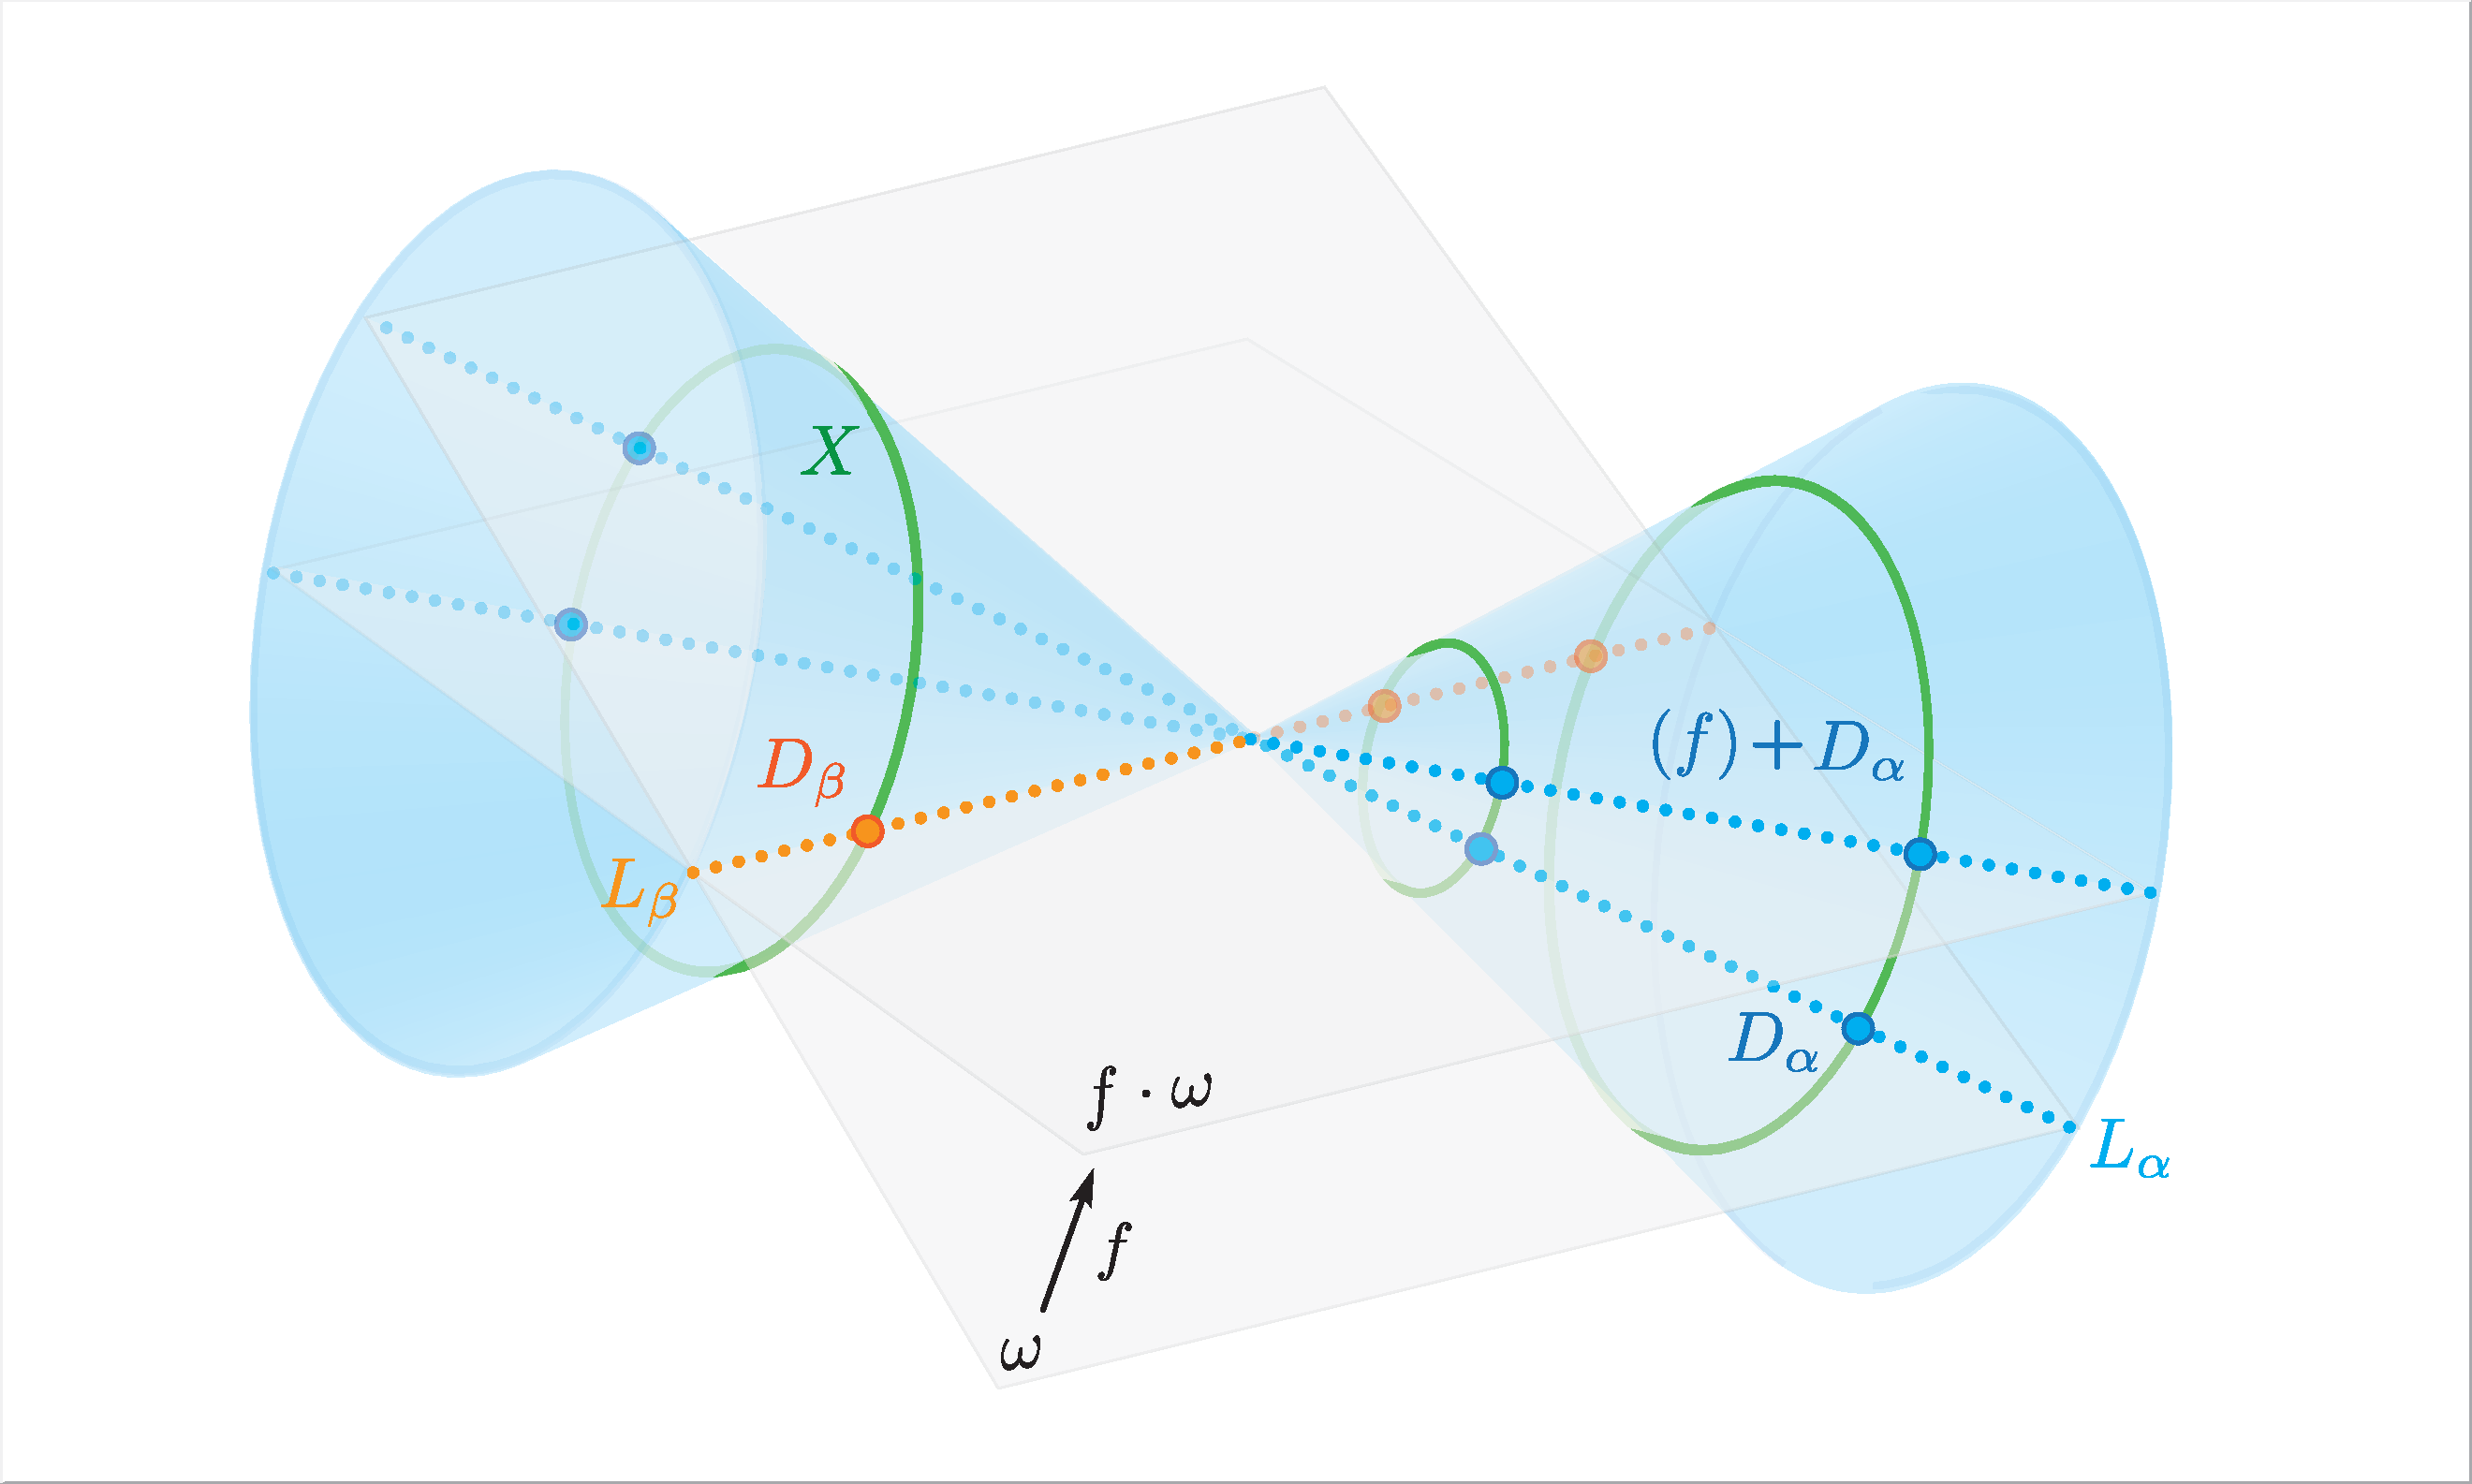
\includegraphics[width=0.85\textwidth]{Cone2.pdf}
			\caption{ A genus $4$ curve contained in a singular ruled quadratic surface -- namely a cone. There is a $\PP^1$-family of hyperplanes passing through $\phi_k(D')$, each one cutting the curve in $D'$ plus a divisor belonging to the unique $g_3^1$. Notice that, in contrast with Figure \ref{fig:Pringles}, every divisor of the $g_3^1$ can be obtained by rotating a plane on the orange axis }
			\label{fig:Cone}
		\end{figure}

		Up to projective equivalence, the singular quadratic surface $Q$ corresponds to the equation
 		$$ X_0^2 = X_1 X_2 $$
 		and can be viewed as the union of a $\PP^1$ family of lines, parametrized by a plane conic, which can be described as
 		$$ A= \begin{cases} X_0=a X_1 \\ X_2=a^2 X_1 \end{cases} $$
 		where the parameter $a$ varies in $\PP^1$. It is easy to check that any two lines $L_\al,\, L_\beta \in A$ intersect in the singular point $[0,0,0,1]$ of $Q$ and, hence, that their span is a plane $H_\alb = \Span(L_\al, L_\beta)$. 
 		Again, such a plane cuts $X$ on the canonical divisor
 		$$ H_\alb \cdot X = D_\al + D_\beta, \qquad D_\al\in L_\al, \; D_\beta\in L_\beta $$
 		and we realize that the situation is closely related to the one of Example \ref{ex:smooth_quadric}. 
 		Reasoning in a similar way one can check that both $D_\al$ and $D_\beta$ give rise to a $g_3^1$, but the crucial difference from the previous Example is that this time there is a unique family of lines and, as a consequence, the two linear series coincide: $|D_\al|=|D_\beta|$.\\
 		The situation is pictured in Figure $\ref{fig:Example2}$, with a $\PP^1$ family of planes \emph{rotating around} $\phi_K(D')$, where each plane intersects the curve in a set of points consisting of $D'$ and a divisor in $|D|$. The reader should notice that a rotation of $H_\w$ by $90$ degrees gives a plane which is tangent to the cone $Q$ and which cuts $X$ in the divisor $2D'$, thus showing that also $D'$ belongs to the linear series $|D|$.

 	
 	\end{example}

 	We therefore see that, in the case of a genus $4$ curve, it is sufficient to count the number of $g_3^1$'s to be able to distinguish between the two possible scenarios described above. More precisely, the variety $G_3^1$ parametrizing linear series of degree $3$ and dimension $1$ is zero dimensional in both cases, but in Example $\ref{ex:smooth_quadric}$ it consists of $2$ distinct points, while it \emph{degenerates} to a unique point in the case of Example $\ref{ex:singular_quadric}$.\\

 	For higher genus the situation becomes more complicated, but still there are many examples in which an analysis of the behaviour of special linear series gives valuable information on the nature of the curve.
	

% ----------------------------------------------------------------------





% this file is called up by thesis.tex
% content in this file will be fed into the main document

%: ----------------------- introduction file header -----------------------
\chapter{The Divisor and Picard schemes}\label{chap:relative_Pic_and_Div}

%: ----------------------- paths to graphics ------------------------

% change according to folder and file names
\ifpdf
    \graphicspath{{figures/}{figures/}{figures/}}
\else
    \graphicspath{{figures/}{figures/}}
\fi

% ----------------------------------------------------------------------
%: ----------------------- introduction content ----------------------- 
% ----------------------------------------------------------------------
%: ----------------------- HELP: latex document organisation
% the commands below help you to subdivide and organise your thesis
%    \chapter{}       = level 1, top level
%    \section{}       = level 2
%    \subsection{}    = level 3
%    \subsubsection{} = level 4
% note that everything after the percentage sign is hidden from output


\nocite{*}


In the first part of this Chapter we will introduce the relative Divisor and Picard functors which, respectively, map a scheme $T$ to flat families of effective Cartier divisors and to families of line bundles with rigidification parametrised by $T$. 
The representability of such functors -- achieved under some particular assumptions -- gives rise to scheme structures for the sets of divisors and line bundles on the curve $X$ and, further, to two universal objects which will be fundamental for the rest of our discussion: the universal divisor $\Delta$ and the universal line bundle $\scL$.\\
Next, exploiting the obtained scheme structure for $\EDiv_X$ and $\Pic_X$, we will compute their tangent spaces. 
It is interesting to observe that the tangent space at a closed point $D$ of the Divisor scheme is naturally isomorphic to the cohomology group $H^0(D)_D$ arising from the sheaf-cohomology of the line bundle $\OXD$ and that, moreover, the tangent space of the Picard scheme at any closed point is simply isomorphic to $H^1(\OX)$ -- the space of first order deformations of line bundles.
This cohomological point of view leads to a description of the \AJJ map by means of the coboundary morphism 
$$ \delta_D : H^0(D)_D \tolong H^1(\OX) $$
appearing in the long cohomology sequence of $\OXD$, from which one realises that the study of linear series is deeply related to the sheaf-cohomology of the curve.\\
Finally, building on the above idea, we will achieve a global cohomological description of the tangent sheaves $T\EDiv_X$ and $T\Pic_X$ --
this is where the universal objects start to reveal their crucial role. In fact, the formal replacement of $D$ by the universal divisor $\Delta$ allows to produce a long cohomology sequence containing the locally-free sheaves $\pi_* \calO_{\Delta}(\Delta)$ and $R^1 \pi_* \calO_Z$, which we will show to be isomorphic to the tangent sheaves of $\EDiv_X$ and $\Pic_X$, respectively. 
Moreover, the \emph{global} coboundary morphism 
$$ \delta: \pi_* \calO_{\Delta}(\Delta) \tolong R^1 \pi_* \calO_Z$$
appearing in the cohomology sequence can be identified with the tangent morphism of sheaves $Tu$, thus giving a global cohomological way to describe the degeneracy loci of the \AJJ map which will be exploited in the next Chapter. 

\section{Working assumptions}\label{sec:assumptions}
	
	Let $k$ be an algebraically closed field of any characteristic. Even though most of what follows can be defined in a more general setting, we restrict our attention to the case in which the following conditions are satisfied:
	$$
		(\star)\;
		\begin{cases}
			\; f:X\to S \text{ is quasi-compact and quasi-separated } \\
			\; f:X\to S \text{ admits a section } \eps:S\to X \\			
			\; f_*\calO_{X_T} \cong \calO_T \text{ for every $S$-scheme } T \\			
		\end{cases}
	$$
	where we abuse notation by writing $f$ for the pullback morphism $X_T\to T$ given by the fibre product. It is easy to show that conditions $(\star)$ are fulfilled in our case of interest, which is described by the following assumptions:
	\begin{assumption}
		For the rest of our discussion, let $X\to S$ be a smooth projective curve of genus $g$ over an algebraically closed field $k=\bar{k}$ and let $S=\Spec(k)$ be the trivial base scheme.
	\end{assumption}


\section{The relative Divisor functor}\label{sec:Div_functor}
	%
	Let $T$ be a scheme over $S$ and let us denote by $X_T$ the fibered product $X\times_S T$. To start, let us introduce the notion of a relative effective Cartier divisors.
	\begin{defi}
		A \textbf{relative effective Cartier divisor} on $X_T/T$ is a closed subscheme $D\subset X_T$ such that its ideal sheaf $\calO_D\subset \OX$ is invertible and the map $\ph: D\to T$ is flat.\\
		Associated to any such divisor we have a map to the natural numbers given by
		$$ \deg_D : T \to \N, \qquad t \mapsto \text{rank of } \ph_*(\calO_D) \text{ as a } \calO_{T,t} \text{ - module } $$
		and, in case of this map being constantly equal to $d\in \N$, we say that $D$ has degree $d$.\\
		The sum $D_1 + D_1$ is defined as the closed subscheme of $X$ corresponding to the sheaf of ideals $\calO_{D_1}\calO_{D_2}\subset \OX$.
	\end{defi}
	We refer to \cite[Tag 01WO]{stacks-project} for further details and for a proof of the fact that relative effective Cartier divisors are closed under the above defined sum.\\
	Based on this notion we now define the contravariant functor $\DivXS$ which maps an $S$-scheme $T$ to the set of families of divisors parametrized by $T$.
	\begin{defi}
		We define the \textbf{relative effective Cartier divisors functor} by
		$$ \DivXS:\Sch_S^{op} \to \Set, \quad T \mapsto \set{ \text{ Relative effective Cartier divisors} \text{ on } X_T/T }. $$
		and the action on morphism by sending an $S$-map $T'\overset{f}\to T$ to the pullback $(1_X\times f)^*$.\\ 
		Moreover, for every $d\in \N$ define the subfunctors $\DivXS^d:\Sch_S \to \Set$ by restricting to divisors of degree $d$.
	\end{defi}
	\begin{rema}
		Notice that composition of morphisms is obviously respected and, further, the flatness of $D\to T$ ensures that the pullback $(1_X\times f)^*D$ is a relative effective Cartier divisor on $X_{T'}/T'$. Hence we see that $\DivXS$ is in fact a (contravariant) functor \\
		Further one can show that, if $\DivXS$ is representable by a scheme $\EDiv_X$, then the subfunctors $\DivXS^d$ are representable by open and closed subschemes $\Dd$ which form a disjoint cover of $\EDiv_X$ -- see Exercise 3.8 of \cite{PICARD} for details.
	\end{rema}
	\begin{notation}
		In the following we will abuse notation by simply writing $f^*$ instead of $(1_X\times f)^*$ , whenever the meaning is clear from the context and no confusion arises.
	\end{notation}
	Under reasonable hypothesis on $X\to S$, the relative Divisor functor turns out to be representable, the representing scheme being an open subscheme of the Hilbert scheme.
	\begin{theo}\label{thm:div_representable}
		If the structure morphism $f:X\to S$ is projective and flat, then the functor $\DivXS$ is representable by an open subscheme of the Hilbert scheme.
	\end{theo}
	\begin{proof}
		A proof can be found for instance in \cite{PICARD} -- see Theorem 3.7.
	\end{proof}
	Therefore under our assumptions -- $X$ a projective curve and $S=\Spec(k)$ -- the relative Divisor functor is representable.\\	

\section{The relative Picard functor}\label{sec:Pic_functor}
	
	We now want to define a relative Picard functor, which extends the concept \emph{Picard group} to flat families of line bundles parametrized by any $S$-scheme $T$. But let us first recall how the classical Picard group is defined:
	\begin{defi}
		Let $X$ be a scheme over a field $k$. We define the \textbf{Picard group} of $X$ as the as the sheaf cohomology group
		$$ \Pic(X) := H^1(X, \OX^*) $$
	\end{defi}
	There are subtle issues involved in the definition of the relative Picard functor and one needs to be careful. A naive definition could be of the form
	$$ T \mapsto \Pic(X_T)/\Pic(T) $$
	but this does not lead to a representable functor, as one can see it only defines a \emph{pre}sheaf with respect to both the \'etale and flat topologies. 
	To solve this problem and hope for a representable Picard functor, one could define it as the sheafification of the above naive one, with respect to a reasonable Grothendieck topology on the category $\Sch_S$. Another strategy, which leads to the same result but is conceptually more transparent, is to get rid of the automorphisms of the objects -- families of line bundles -- we want to parametrize with our functor. 
	We will adopt this latter approach, thus restricting our attention to the class of rigidified line bundles which we now introduce.
	\begin{defi}
		Let $f:Y\to B$ be a scheme, $\eps:B\to Y$ a section of $f$ and $L$ a line bundle over $Y$.
		A \textbf{rigidification of $L$ along} $\eps$ is an isomorphism $\al: \eps^*L \toiso \calO_B $.
		We define a \textbf{rigidified line bundle} on $Y/B$ to be a pair $(L,\al)$ consisting of a line bundle on $Y$ together with a rigidification along $\eps$.
	\end{defi}
	\begin{comment}
		A \textbf{rigidified line bundle} on $X/T$ is a line bundle $L\to X_T$ together with a rigidification $\al: \eps_T^*L \toiso \calO_T $ along $\eps_T$, where $\eps_T:T\to X_T$ is the section of $X_T\to T$ induced by a given section $\eps:S\to X$.
	\end{comment}
	One can show that, under our hypothesis, any such line bundle can be written in the form $\calO(D)$ for an effective Cartier divisor $D$ on $Y/B$. Thus we define the \textbf{degree} of a rigidified line bundle $(L,\al)$ to be the degree of the corresponding divisor.\\

	Going back to our situation $(\star)$ of a scheme $f:X\to S$ with a section $\eps:S\to X$ at our disposal, for every $T\in \Sch_S$ there is a canonical way to rigidify line bundles on $X_T/T$ along the induced section $\eps_T$ -- which by abuse of notation we will also denote by $\eps$. 

	\begin{equation*}
	\begin{tikzpicture}[node distance=5em, auto] %SQUARE
		\node (A) 															{$X_T$};
		\node (B) 	[right of=A, xshift=3em]		{$T$};
	  \node (C) 	[below of=A] 								{$X$};
	  \node (D) 	[right of=C, xshift=3em] 		{$S$};
	  %
	  \draw[-stealth, bend left=15, looseness=1]						(A)		to node {$f$} 			(B);
	  \draw[-stealth, bend left=15, looseness=1]						(B)		to node {$\eps$} 	(A);
	  \draw[-stealth]																				(A)		to node {} (C);
	  \draw[-stealth]																				(B)		to node {} (D);
	  \draw[-stealth, bend right=15, looseness=1, swap]			(D)		to node {$\eps$}		(C);
	  \draw[-stealth, bend right=15, looseness=1, swap]			(C)		to node {$f$} 			(D);
	\end{tikzpicture}
	\end{equation*}

	In fact, given a line bundle $M$ over $X_T$, one can obtain a line bundle $(L,\al)$ with rigidification along $\eps$ by setting
	$$ L:= M\otimes f^* \eps^* M^{-1} . $$
	Indeed, recalling that by definition of section $f\circ\eps \equiv 1$, we find that
	$$ 
	\eps^* L 
	= 
	\eps^*M\otimes \eps^* f^* \eps^* M^{-1} 
	= 
	\eps^*M\otimes (f\circ\eps)^* \eps^* M^{-1}
	=
	\eps^* (M\otimes M^{-1})
	=
	\calO_T  
	$$
	as desired.
	The key feature of rigidified line bundles is that they do not admit nontrivial automorphisms, as we show in Proposition \ref{prop:rigid} of Appendix A.\\

	We are now ready to define the relative Picard functor:
	\begin{defi}
		We define the \textbf{relative Picard functor} by the assignment
		$$ \PicXS:\Sch_S^{{op}} \to \Ab, \qquad T \mapsto \set{ \text{Rigidified line bundles}\text{ on } X_T/T } $$
		and the action on morphism by sending an $S$-map $T'\overset{f}\to T$ to the pullback $(1_X\times f)^*$.\\ 
		Moreover, for every $d\in \N$, we define the subfunctors $\PicXS^d:\Sch_S \to \Set$ by restricting to line bundles of degree $d$.
	\end{defi}
	\begin{rema}
		Notice that composition of morphisms is obviously respected and, further, it is a well known fact that line bundles are stable under pullbacks. Hence we see that $\PicXS$ is in fact a (contravariant) functor.
	\end{rema}	
	It can be shown (see for instance Section 8.1 of \cite{BOSCH}) that conditions $(\star)$ imply the representability of $\PicXS$ and, moreover, that for every $S$-scheme $T$ there is a natural isomorphism
	\begin{equation}\label{eq:PicXS}
		\PicXS(T) \;\cong\; \Pic(X_T) / \operatorname \Pic(T)
	\end{equation}

\section{Universal divisor and universal line bundle}
	%
	As remarked above, under our hypothesis Theorem \ref{thm:div_representable} applies, therefore $\DivXS^d$ is representable and we will denote the representing $S$-scheme by $\Dd$, which is unique up to unique isomorphism. For $\Dd$ to be the representing scheme it means that there are canonical isomorphisms
	$$ \DivXS(T) \;\cong\; \HomS(T,\Dd), \quad \forall \;T\in \Sch_S $$
	and a universal object $\Delta \in \DivXS(\Dd)$ with the property that to every morphism $f\in \HomS(T,\Dd)$ corresponds a unique $D\in \DivXS(T)$ given as the pullback $f^*(\Delta)$ of $\Delta$ via $f$. This is the universal property of $\Delta$. 
	Notice that there is a bijection between the set of closed points of $\Dd$ and the set of effective divisors of degree $d$ on $X$. In particular with $T=S$, for any divisor $D\in \Dd$ there is a unique canonical $S$-map $f:S\into\Dd$ such that $f^*(\Delta) = D$.\\

	The same reasoning applies to line bundles: as soon as $\PicXS^d$ is representable we get a representing $S$-scheme $\Pd$ unique up to unique isomorphism (whose points are line bundles of degree $d$ on $X/S$) and a universal line bundle $\scL \in \PicXS(\Pd)$. Notice that, under our hypothesis, the relative Picard functor $\PicXS$ is representable and identification $\eqref{eq:PicXS}$ holds.\\

	Due to their importance in the rest of our discussion, we summarize below the nature of the universal objects we just obtained, in a concise fashion: 
	\begin{notation}
		The above universal objects are denoted by
		$$
			\begin{array}{ l c l }
				\Delta\;\subset\; X\times \Dd \qquad &\leadsto& \textbf{ Universal divisor }
				\\\\
				\scL \longrightarrow X\times \Pd \qquad &\leadsto& \textbf{ Universal line bundle }
			\end{array}
		$$
	\end{notation}\vspace{1em}
	It is interesting to notice that, as we will show in the next sections, these universal objects can be used to describe the tangent sheaves of the Divisor and Picard schemes.\vspace{1em}

\section{Tangent spaces of $\Dd$ and $\Pd$ }\label{sec:tgnt_spaces}
	%
	Within the categorical setting introduced in the previous Sections, the Abel-Jacobi map can be seen as a natural transformation of functors between $\DivXS$ and $\PicXS$.
	\begin{defi}
		We define the Abel-Jacobi map (also known as the Albanese map) as the natural transformation of functors
		$$ u: \DivXS \to \PicXS, \qquad \scr{D} \mapsto \calO(\scr{D}).$$
	\end{defi}
	For every $d\in \N$ the classical Abel-Jacobi map induces a morphism in the category of schemes over $S$, between the representing schemes
	$$ u :  \Dd \to \Pd, \qquad D \mapsto \OXD $$
	and, in order to study its tangent map at a closed point $D\in \Dd$
	$$ \TDu : T_D \Dd \to T_{u(D)} \Pd \,, $$
	we should, first of all, understand the above tangent spaces. A very useful tool for this purpose is the ring of the dual numbers $ k_\eps = k[\eps]/\eps^2 $ and the associated fibred product 
	$$ X_\eps := X \underset{{S}}\times {\Spec(k_\eps)}. $$ 
	Moreover, for any $k$-scheme $P$ with a rational point $e$, denote by $P(k_\eps)_e$ the set of all $k$-maps from the \emph{free tangent vector} $\Spec(k_\eps)$ to $P$ which are supported at $e$. \\

	In this situation Lemma \ref{lemm:tng_sch} of Appendix A shows that the $k$-vector space $P(k_\eps)_e$ is in fact isomorphic to the tangent space to $P$ at the point $e$, in formula
	$$ P(k_\eps)_e \; \cong \; T_e P. $$
	Further Lemma \ref{lemm:tng_grp_sch} of Appendix A tells us that, if $P$ is a group scheme, then the tangent space at the identity element $e$ is simply given by
	$$ T_e P \;\cong\; \ker \Big( P(k_\eps) \to P(k) \Big). $$
	In order to describe the tangent space of $ \Pd$ it is useful to introduce the normal sheaf associated to a divisor, by means of the following 
	\begin{defi}
		The \textbf{normal sheaf} associated to a divisor $D\in  \Pd$ is defined as
		$$ \ODD := \OXD \otimes \calO_D. $$
		We remark that, even though $\ODD$ is a sheaf on $D$, we will often treat it as a sheaf on $X$ by implicitly pushing it forward via the natural inclusion of $D$ into $X$. 
	\end{defi}
	\begin{notation}
		With the aim of making our notation lighter, we will often write 
		$$ H^i(D)_{D} \equiv H^i(X,\ODD)$$ 
		for the $i$-th cohomology group of the normal sheaf.
	\end{notation}
	\begin{rema}\label{rema:div_ses}
		The ideal sheaf of $\calO_D$ is $\OX(-D)$, so we have a natural \ses
		$$ \SES{\OX(-D)}{\OX}{\calO_D} $$
		and, since tensoring with the invertible sheaf $\OXD$ leaves the sequence exact, we get
		$$ \SES{\OX}{\OXD}{\ODD}. $$			
	\end{rema}
	The following proposition shows that the normal sheaf $\ODD$ is the house of the infinitesimal deformations of a divisor $D$, so that the tangent space of $\Dd$ at $D$ is just its space of global sections $\HDD$.
	\begin{prop}\label{prop:tgn_div}
		Let $D$ be a closed point of $ \Dd$. We have an isomorphism of vector spaces
		$$ T_D \Dd \cong \HDD. $$
	\end{prop}
	\begin{proof}
		From Lemma \ref{lemm:tng_sch} of Appendix A we know that the tangent space $T_D \Dd = T_D\DivXS(k)$ coincides with $ \DivXS(k_\eps)_D$, which can be described as the vector space
		
		$$ 
		V = \set{\parbox{8.2cm}{
		Relative effective Cartier divisors on $X_\eps / k_\eps$ 
		whose pull-back to the closed fibre $X\subset X_\eps$ is $D$.
		}}
		\vspace{0.5em}
		$$

		Let $G_i \in H^0(U_i,\OX(-D)) $ be local equations for $D$ over an open cover $U_i$. Then an element of $V$ has local equations
		$$ F_i = G_i + \eps H_i, \qquad H_i \in H^0(U_i,\OX) $$
		satisfying the glueing condition $F_i = (\text{unit})\cdot F_j$ on $U_{i,j}$. Equivalently, such conditions can be expressed as
		$$ G_i + \eps H_i = (a_{i,j} + \eps b_{i,j})\cdot (G_j + \eps H_j) $$
		for some $b_{i,j} \in H^0(U_{i,j},\OX)$ and $ a_{i,j} \in H^0(U_{i,j},\OX^*)$, which implies that
		$$ G_i = a_{i,j} G_j \AND H_i = a_{i,j} H_j + b_{i,j}G_j. $$
		It follows that the assignment $F_i \mapsto H_i/G_i$ is well-defined, since the identity
		$$ \frac{H_i}{G_i}-\frac{H_j}{G_j} = b_{i,j}\cdot a_{j,i} $$
		ensures that $\{H_i/G_i \} $ glues to a global section of $\ODD$. It is easy to check that this gives a bijections of vector spaces.
	\end{proof}
	We now turn to the tangent space of the Picard scheme, which actually admits a simpler description.
	\begin{prop}\label{prop:tgn_pic}
		Let $L$ be a closed point of $ \Pd$ and assume conditions $(\star)$ of Section \ref{sec:assumptions} are met. Then we have an isomorphism of vector spaces
		$$ T_L \Pd \cong H^1(\calO_X). $$
	\end{prop}
	\begin{proof}
		First of all notice that $\Pic = \sqcup_{d\in \N}\Pd$ is a group scheme, therefore the tangent space at every point $L$ is canonically isomorphic to the tangent space at the identity element $ 0\in \Pic^0_X = \PicXS^0(k)$.
		Hence, from Lemma \ref{lemm:tng_grp_sch} of Appendix A we know what we are looking for: the kernel of the map $ \PicXS(k_\eps)\to  \PicXS(k)$. In order to compute it, consider the truncated exponential sequence
		$$ \SES{\OX}{\calO_{X_\eps}^*}{\OX^*}, $$
		where the first map is the exponentiation $e: f\mapsto 1+\eps f$. Notice that this map enjoys the key property of the classical exponential, as we have 
		$$ e(f + g) = 1+\eps(f+g) = (1+\eps f)\cdot(1+\eps g) = e(f) \cdot e(g) $$
		so that its name is justified. The above sequence splits using the natural inclusion of $\OX^*$ into $\calO_{X_\eps}^*$, so we obtain a \ses in cohomology of degree $1$
		$$ \SES{H^1(\OX)}{H^1(\calO_{X_\eps}^*)}{H^1(\OX^*)}. $$
		Now, the fact that conditions $(\star)$ are satisfied implies that the natural identification \eqref{eq:PicXS} holds, thus giving isomorphisms
		$$ \PicXS(k) \cong \Pic(X) = H^1(\OX^*) \AND \PicXS(k) \cong \Pic(X_\eps) = H^1(\calO_{X_\eps}^*)\,. $$
		Therefore we have the following commutative diagram with exact rows, where the two vertical arrows on the right are isomorphisms and thus the same holds for the induced vertical map between the kernels.
		$$
		\begin{tikzpicture}[node distance=4em, auto]
			\node (O) 															{$0$};
			\node (A) 	[right of=O, xshift=2em]		{$H^1(\OX)$};
			\node (A2) 	[right of=A]								{$\;$};
			\node (B) 	[right of=A2]								{$H^1(\calO_{X_\eps}^*)$};
			\node (B2) 	[right of=B]								{$\;$};
		  \node (C) 	[right of=B2] 							{$H^1(\OX^*)$};
		  \node (OO) 	[right of=C, xshift=2em] 		{$0$};
		  \node (O') 	[below of=O] 								{$0$};
		  \node (A') 	[below of=A] 								{$T_0 \PicXS(k)$};
		  \node (B') 	[below of=B] 								{$ \PicXS(k_\eps)$};
		  \node (C') 	[below of=C] 								{$ \PicXS(k)$};
		  \node (OO') [below of=OO] 							{$0$};
		  \draw[-stealth] 				(O)	to node {} (A);
		  \draw[-stealth]					(A)		to node {} (B);
		  \draw[-stealth]					(B)		to node {} (C);
		  \draw[-stealth]					(C)		to node {} (OO);
		  \draw[-stealth]					(O')	to node {} (A');
		  \draw[-stealth]					(A')	to node {} (B');
		  \draw[-stealth]					(B')	to node {} (C');
		  \draw[-stealth]					(C')	to node {} (OO');
		  \draw[-stealth][dashed]	(A)	to node {} (A');
		  \draw[-stealth]					(B)		to node {} (B');
		  \draw[-stealth]					(C)		to node {} (C');
		\end{tikzpicture}
		$$
		Finally, one can easily check that the above dashed isomorphism is in fact an isomorphism of vector spaces.
	\end{proof}

\section{Tangent bundles of $\Dd$ and $\Pd$ }
	In the last section we gave an entirely cohomological description of the tangent spaces of both $\Dd$ and $\Pd$. We will now show that we can actually do much better, giving a cohomological description for the tangent \emph{sheaves} of those varieties, thus achieving a global analogue of the identifications obtained, fiberwise, in the last section. \\
	We start with a Lemma showing that the sheaves we are interested in are locally-free.

	\begin{notation}
		In order to make our notation shorter, in the following we will use write simply $Z$ to denote the product $X\times \Dd$, and we will write $\pi:Z\to \Dd$ for the natural projection on the second factor. 
	\end{notation}

	\begin{defi}
		A \textbf{locally free sheaf} of rank $n$ on a scheme $Y$ is defined as an $\calO_Y$-module $\scr{F}$ that is locally a free sheaf of rank $n$. More precisely, there is an open cover $\{U_i\}$ of $Y$ such that over each $U_i$ we have an isomorphism $\scr{F}_{\mid U_i} \cong \calO_{U_i}^{\oplus n}$.
	\end{defi}

	\begin{rema}\label{rema:smoothness}
		It is a well known fact that, in our case of a smooth projective curve over an algebraically closed field, the representing schemes $\Dd$ and $\Pd$ are in fact smooth varieties in any characteristic. We do not prove these facts here but we refer to the literature -- see for instance the discussion in Chapter 5 of $\cite{PICARD}$. Therefore it follows that the tangent sheaves $T\Dd$ and $T\Pd$ are locally-free.\\
		Moreover, we remark that the quasi-coherent sheaves $\pi_* \calO_{\Delta}(\Delta)$ and $R^1\pi_*\calO_Z$ are locally-free, as will show in Proposition \ref{prop:free_pres}.\\
	\end{rema}

	Starting from the tangent sheaf of the Divisor scheme, our strategy is to pass from a single divisor $D$ to the universal divisor $\Delta$, making the formal replacement 
	$$ \HDD, \text{ vector space } \qquad \large\mapsto \qquad \pi_* \calO_{\Delta}(\Delta), \text{ locally free sheaf }$$
	
	\begin{prop}
		There is a canonical isomorphism of sheaves $T\Dd \cong \pi_* \calO_{\Delta}(\Delta)$.
	\end{prop}
	\begin{proof}
		Let $\tilde{\pi}$ denote the restriction of $\pi:X\times\Dd\to \Dd$ to the divisor $\Delta$ and look at the diagram of the closed immersion
		$$
		\begin{tikzpicture}[node distance=4em, auto]
			\node (A) 														{$\Delta$};
			\node (B) 	[right of=A, xshift=3em]	{$X\times\Dd$};
		  \node (C) 	[below of=B] 							{$\Dd$};
		  %
		  \draw[right hook-stealth]				(A)		to node {} 								(B);
		  \draw[-stealth]									(B)		to node {$\pi$} 					(C);
		  \draw[-stealth][swap]						(A)		to node {$\tilde{\pi}$} 	(C);
		\end{tikzpicture}
		$$
		from which we readily observe that we have natural identifications
		$$ 
		\tilde{\pi}^* (T \Dd) = (\pi^* T \Dd)_{\mid_\Delta} 
		\AND 
		T (X\times\Dd)_{\mid_\Delta} = (\pi^* T\Dd)_{\mid_\Delta} \oplus (\operatorname{Pr}^*_X TX)_{\mid_\Delta} .
		$$
		Moreover, since $\calO_{\Delta}(\Delta)$ is the normal bundle of the divisor $\Delta$, there is a natural map
		$$ T(X\times \Dd) \tolong \calO_{\Delta}(\Delta) $$
		which, in light of the above identifications, gives a map from $\pi^*T\Dd $ to $ \calO_{\Delta}(\Delta)$ obtained by restriction. Therefore by the adjunction between $\pi_*$ and $\pi^*$ we find what we were looking for: a morphism		
		$$ T\Dd \tolong \pi_* \calO_{\Delta}(\Delta). $$
		As remarked in Remark \ref{rema:smoothness}, the two sheaves in question are locally free of finite rank, therefore it is sufficient to show that the above global map induces isomorphisms on each fibre. One can check that, in fact, this global morphisms restricts on every fibre to the linear map
		$$ T_D \Dd \toiso \HDD $$
		which we proved to be an isomorphism in Proposition \ref{prop:tgn_div}, thus achieving the desired conclusion.
	\end{proof}
	We now turn to the case of the Picard scheme, in which our strategy is in some sense to make the formal replacement
	$$ H^1(\OX), \text{ vector space } \qquad \large\mapsto \qquad R^1 \pi_* \calO_Z, \text{ locally free sheaf }$$
	\begin{prop}
		There is a canonical isomorphism of sheaves $u^* T\Pd \cong R^1 \pi_* \calO_Z$.
	\end{prop}
	\begin{proof}
		First of all recall from Proposition \ref{prop:tgn_pic} that we have an isomorphism
		$$ T_0 \PicXS \cong H^1(X, \OX)$$
		then notice that, since $\PicXS$ is a group variety, its tangent sheaf is constant with fibers $H^1(X, \OX)$. The same is true if we restrict to the subscheme $\Pd$, thus we see that $ T \Pd $ is the constant sheaf $\underline{H^1(X,\OX)}$ over $\Pd$. \\

		Actually, we claim that $R^1 \pi_* \calO_{Z}$ is also constant with fibers $H^1(X, \OX)$. To see this consider the base change diagram
		$$
		\begin{tikzpicture}[node distance=5em, auto]
			\node (A) 															{$Z$};
			\node (B) 	[right of=A, xshift=2em]		{$X$};
		  \node (C) 	[below of=A] 								{$\Dd$};
		  \node (D) 	[right of=C, xshift=2em] 		{$S$};
		  %
		  \draw[-stealth]					(A)		to node {} (B);
		  \draw[-stealth][swap]		(A)		to node {$\pi$} (C);
		  \draw[-stealth]					(B)		to node {$f$} (D);
		  \draw[-stealth]					(C)		to node {$g$} (D);
		\end{tikzpicture}
		$$
		and notice that, since we are assuming $S=\Spec(k)$, the structure morphism $f:X\to S$ is flat. Hence the above diagram describes a flat base change and thus ( use Proposition 9.3 of $\cite{HAG}$ for instance ) we get
		$$ R^1 \pi_*\calO_{Z} \cong g^* \left( R^1f_*\OX \right) \cong  g^* H^1(X,\OX), $$
		from which we deduce that $R^1\pi_* \calO_{Z}$ is the constant sheaf with fibers $H^1(X,\OX)$ over $\Dd$. Therefore it follows that $ u^* T \Pd \cong R^1 \pi_* \calO_{Z} $ .
 	\end{proof}

\section{Cohomological description of the Abel-Jacobi map}
	In this section we will achieve a purely cohomological description of the tangent map $Tu$ of the Abel-Jacobi map, first fiberwise and then globally.
	\subsection{Fiberwise description}
		In section \ref{sec:tgnt_spaces} we showed that, on every closed point $D$, the tangent morphism $\TDu$ is a linear map $\HDD\to H^1(\OX)$, which looks pretty familiar. Indeed from the natural \ses	of sheaves of Remark \ref{rema:div_ses}, i.e.
		$$ \SES{\OX}{\OXD}{\ODD} $$
		we get, observing that $H^1(X,\ODD)$ is trivial since $D$ is $0$-dimensional, the following \les in cohomology
		\begin{equation}\label{eq:abel_les}
			0\to H^0(\OX) \to H^0(D) \to \HDD \overset{\delta_D}\longrightarrow H^1(\OX) \to H^1(D) \to 0
		\end{equation}
		and we are going to show that the coboundary map $\delta_D$ can be identified with $\TDu$.
		\begin{prop}\label{prop:delta_u}
			Under the isomorphisms of Propositions \ref{prop:tgn_div} and \ref{prop:tgn_pic}, the maps $\delta_D$ and $\TDu$ can be identified.
		\end{prop}
		\begin{proof}
			We want to prove the commutativity of the following diagram
			$$
			\begin{tikzpicture}[node distance=5em, auto]
				\node (A) 									{$\HDD$};
				\node (A2) 	[right of=A]		{$\;$};
				\node (B) 	[right of=A2]		{$T_D \Dd$};
			  \node (C) 	[below of=A]	 	{$H^1(\OX)$};
				\node (C2) 	[below of=A2]		{$\;$};
			  \node (D) 	[below of=B] 		{$T_{u(D)} \Pd$};
			  \draw[-stealth] 				(A)		to node {$\sim$} 				(B);
			  \draw[-stealth]					(C)		to node {$\sim$} 				(D);
			  \draw[-stealth]					(A)		to node {$\delta_D$} 	(C);
			  \draw[-stealth]					(B)		to node {$\TDu$} 			(D);
			\end{tikzpicture}
			$$
			where the lower horizontal map is the exponentiation $f\mapsto 1+\eps f$.\\
			Let $G_i$ be local equations for $D$ and $H_i/G_i$ represent a global section of $\HDD$. The coubandary map acts on it as
			$$ \delta_D\left(\frac{H_i}{G_i}\right) =  \frac{H_i}{G_i}-\frac{H_j}{G_j}. $$
			On the other hand, $H_i/G_i$ is identified with the element of $T_D \Dd$ defined by local equations $F_i = G_i + \eps H_i$ and gets mapped through $\TDu$ to the element of $T_{u(D)} \Pd$ with transition functions given by
			$$ \sigma_{i,j} = F_i / F_j. $$
			This can be expanded (here's the trick!) as
			\begin{eqnarray*}
				\sigma_{i,j} &=& (G_i + \eps H_i)/(G_j + \eps H_j) \\
				&=& G_i G_j^{-1}\cdot(1+\eps H_i/G_i)\cdot(1-\eps H_j/G_j) \\
				&=& G_i G_j^{-1}\cdot(1+\eps (H_i/G_i - H_j/G_j)).
			\end{eqnarray*}
			Now notice that $G_i G_j^{-1}$ represents a section of $\OXD$, thus we can divide them out: this just means translating $\sigma_{i,j} $ back to the origin of $ \Pd$. We are left with
			$$ 1 + \eps\left( \frac{H_i}{G_i}-\frac{H_j}{G_j} \right), $$
			which is the image under the exponential map of $\delta_D(H_i/G_i)$, as we wanted.
		\end{proof}
		We can now rewrite the \les \eqref{eq:abel_les} as
		\begin{equation}\label{eq:local_diagram}
		\begin{tikzpicture}[node distance=5em, auto]
			\node (O) 									{$0$};
			\node (A) 	[right of=O]		{$H^0(D)/k$};
			\node (B) 	[right of=A, xshift=2em]		{$H^0(D)_D$};
		  \node (C) 	[right of=B, xshift=4em] 		{$H^1(\OX)$};
		  \node (D) 	[right of=C, xshift=2em] 		{$H^1(D)$};
		  \node (OO) 	[right of=D] 		{$0$};
		  \node (O') 	[below of=O] 		{$0$};
			\node (A') 	[below of=A] 		{$ T_D |D|$};
		  \node (B') 	[below of=B] 		{$ T_D \Dd$};
		  \node (C') 	[below of=C] 		{$ T_{\OXD} \Pd $};
		  \node (D') 	[below of=D] 		{$\;$};
			\draw[-stealth] 				(O)		to node {} (A);
		  \draw[-stealth]					(A)		to node {} (B);
		  \draw[-stealth]					(B)		to node {$\delta_D$} (C);
		  \draw[-stealth]					(C)		to node {} (D);
			\draw[-stealth]					(D)		to node {} (OO);
			\draw[-stealth] 				(O')	to node {} (A');
		  \draw[-stealth]					(A')	to node {} (B');	  
		  \draw[-stealth]					(B')	to node {$T_D u$} (C');
		  \draw[-stealth][swap]		(A)		to node {$\cong$} (A');
		  \draw[-stealth][swap]		(B)		to node {$\cong$} (B');
		  \draw[-stealth]					(C)		to node {$\cong$} (C');
		\end{tikzpicture}
		\end{equation}	
		from which we make the following observations:
		\begin{enumerate}[i)]
			\item The dimension of the Picard scheme is bounded by $h^1(\OX)$ and equality holds \ABiff $ \Pd$ is smooth, at any point and hence everywhere. In the case of $X$ being a smooth curve of genus $g$, recall that by definition $h^1(\OX)=h^0(K)=g$;
			\item The kernel of $\TDu$ is $H^0(D)/k \cong \PP H^0(D)$, so one notices that $u$ is constant on linear series. This is the content of Abel's theorem.
		\end{enumerate}

	\subsection{Global description}

		In the last Section we showed that the tangent spaces of $\Dd$ and $\Pd$ can be seen as cohomology groups and, further, that the tangent map $\TDu$ at any point $D$ is a linear map of vector spaces. 
		We now want to make this idea global, aiming for a cohomological description of the tangent sheaves of $\Dd$ and $\Pd$ and the sheaf morphism $\Tu$. 
		To do so, we will make use of the universal divisor $\Delta$ and the universal line bundle $\scL$ to obtain two exact sequences of sheaves, which will serve as global analogues of \eqref{eq:abel_les}. 
		Moreover, we will show that the last part of these sequences are free presentations, a fact that will be of crucial importance for the definition of the moduli varieties parametrising linear series and, in general, for the rest of our discussion.\\

		\begin{defi}\label{def:Gamma}
			Choose a divisor $M = \sum_{i=1}^m P_i$ consisting of $m \geq 2g-d-1$ distinct points of $X$, then define the product divisor 
			$$\Gamma := M\times \Pd$$
		\end{defi}	


		\begin{prop}\label{prop:free_pres}
			Let $\pi : X\times \Dd \to \Dd$ and $\nu : X\times \Pd \to \Pd$ denote the natural projections on the second factor. Then the exact sequence of sheaves
			\begin{equation}\label{eq:univ_div_seq}
				\pi_* \calO_{\Delta}(\Delta)\overset{\delta}\to R^1 \pi_* \calO_Z \to R^1 \pi_* \calO_Z(\Delta) \to 0
			\end{equation}
			is a free presentation of $R^1 \pi_* \calO_Z(\Delta)$, while the exact sequence of sheaves
			\begin{equation}\label{eq:univ_lb_seq}
				\nu_{*} \scL(\Gamma)\to \nu_{*} \scL(\Gamma) / \scL \to R^1 \nu_{*} \scL \to 0
			\end{equation}		
			is a free presentation of $R^1 \nu_{*} \scL$.
		\end{prop}
		\begin{proof}
			We start by looking at the natural \ses
			\begin{equation}\label{eq:univ_div_ses}
				\SES{\calO_Z}{\calO_Z(\Delta)}{\calO_\Delta(\Delta)} 
			\end{equation}
			associated to the universal divisor, which is in some sense the global analogue of the second sequence appearing in Remark \ref{rema:div_ses}. Since $D$ is $0$-dimensional and $h^1(D_D)= 0$, Proposition \ref{prop:no_jumps} of Appendix A implies that $R^1 \pi_* \calO_{\Delta}(\Delta) = 0$, therefore the last part of the direct image sequence of \ref{eq:univ_div_ses} is given by
			$$
				\pi_* \calO_{\Delta}(\Delta)\overset{\delta}\to R^1 \pi_* \calO_Z \to R^1 \pi_* \calO_Z(\Delta) \to 0.
			$$
			As we showed in Section \ref{sec:tgnt_spaces}, for every $D\in \Dd$ the cohomology groups
			$$ H^0(X, D_D) \cong T_D \Dd \AND H^1(X, \OX) \cong T_{\OXD} \Pd $$
			are fiberwise vector spaces of dimensions $d$ and $g$. Hence Proposition \ref{prop:no_jumps} implies that $\pi_* \calO_{\Delta}(\Delta)$ is locally free of rank $d$ and that $R^1 \pi_* \calO_Z$ is locally free of rank $g$, thus showing that \eqref{eq:univ_div_seq} is in fact a \textbf{free} presentation.
			\\
			Moving towards the second sequence, notice that we have the natural \ses 
			\begin{equation}\label{eq:univ_lb_ses}
				\SES{\scL}{\scL(\Gamma)}{\scL(\Gamma)/\scL} 
			\end{equation}
			and, since by Lemma \ref{lemm:trivial_R1} of Appendix A we have $R^1 \nu_{*} \scL(\Gamma) = 0$, the corresponding direct image sequence is given by
			\begin{equation}\label{eq:univ_lb_direct_image}
				0 \to \nu_{*}\scL \to \nu_{*} \scL(\Gamma)\overset{\gamma}\tolong \nu_{*} \scL(\Gamma) / \scL \to R^1 \nu_{*} \scL \to 0 \,.
			\end{equation}
			Moreover, since for every $L\in \Pd$ the \RR implies $h^0(X, L(M)) = d+m-g+1 $, another application of Proposition \ref{prop:no_jumps} implies that  $\nu_{*} \scL(\Gamma)$ is locally free of rank $d+m-g+1$. 
			Finally, we notice that $\scL(\Gamma) / \scL$ can be seen as a line bundle on $\Gamma$, so it follows that $\nu_{*} \scL(\Gamma) / \scL$ is locally free of rank $m$, as $\nu$ restricts to a finite locally free morphism of degree $m$ on $\Gamma\subset X\times \Pd$.
		\end{proof}

		\begin{figure}[ht]
				\centering
				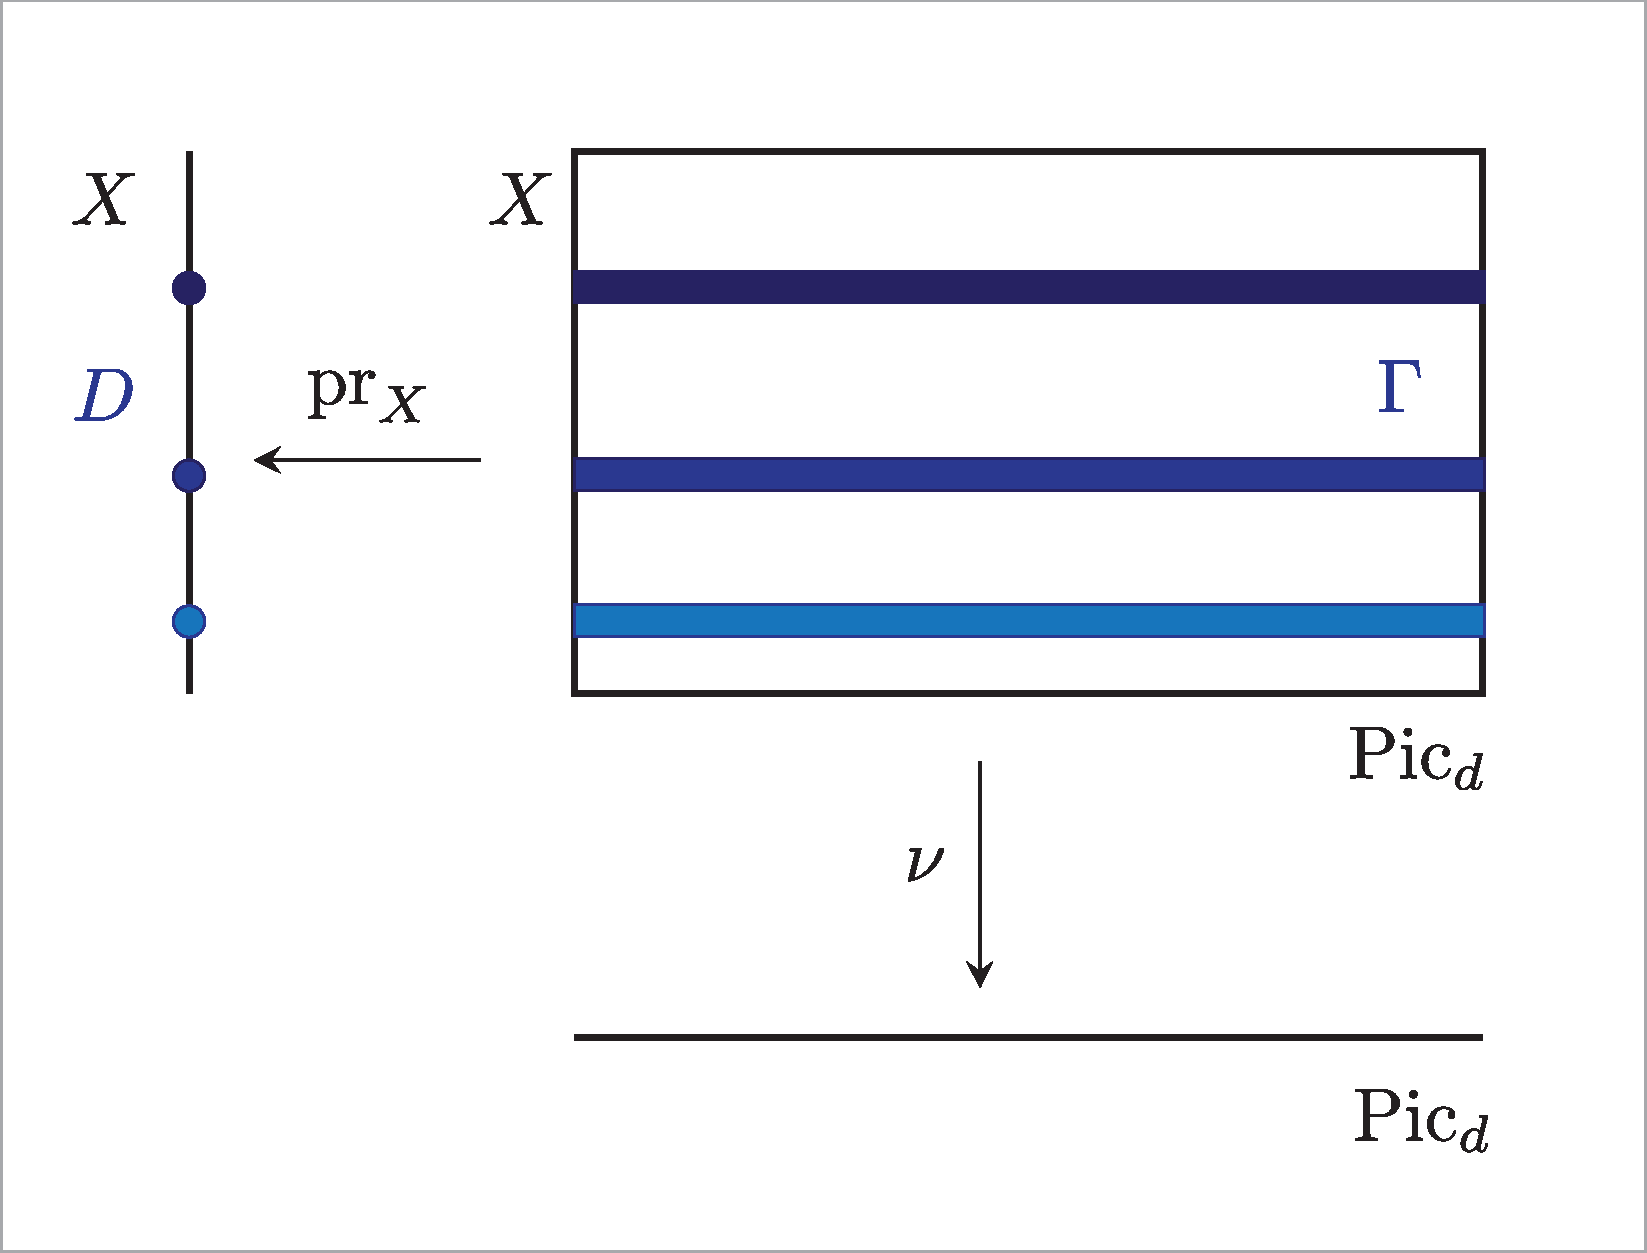
\includegraphics[width=0.85\textwidth]{Locally-free-of-degree-m.pdf}
				\caption{The projection $\nu$ restricts to a finite locally free morphism of degree $m$ on the product $\Gamma\subset X\times \Pd$ }
				\label{fig:locally_free_morphism}
		\end{figure}
		
		\begin{rema}\label{rema:ranks}
			During the proof of the above Lemma we showed that the ranks of the first two bundles appearing in the presentation \eqref{eq:univ_lb_seq} are $d+m-g+1$ and $m$. Keep it in mind, because this fact will be exploited during the proof of the Connectedness Theorem.
		\end{rema}

		Collecting the results of this Chapter, we are now able to write down a commutative diagram in the category of coherent sheaves which is in some sense the \emph{global version} of \eqref{eq:local_diagram} and, thus, gives an identification of the coboundary map $\delta:\pi_* \calO_\Delta(\Delta)\to R^1\pi_*\calO_Z$ with the morphism of locally free sheaves $\Tu:T \Dd\to u^* T \Pd$, representing the tangent map of the \AJJ map $u$ restricted to divisors of degree $d$.

		$$
		\begin{tikzpicture}[node distance=8em, auto]
			%node (O) 									{$0$};
			\node (A) 									{$\pi_* \calO_Z(\Delta)$};
			%node (A2) 	[right of=A]		{$\;$};
			\node (B) 	[right of=A]		{$\pi_* \calO_\Delta(\Delta)$};
			%node (B2) 	[right of=B]		{$\;$};
		  \node (C) 	[right of=B] 	{$R^1 \pi_* \calO_Z$};
			%\node (C2) 	[right of=C] 		{$\;$};
		  \node (D) 	[right of=C] 	{$R^1 \pi_* \calO_Z(\Delta)$};
			%\node (OO) 	[right of=D] 		{$0$};
		  %\node (O') 	[below of=O] 		{$\;$};
		  \node (A') 	[below of=A] 		{$\;$};
		  \node (B') 	[below of=B, yshift=3em] 		{$ T \Dd$};
		  \node (C') 	[below of=C, yshift=3em] 		{$ u^* T \Pd $};
		  \node (D') 	[below of=D] 		{$\;$};
			%\node (OO') [below of=OO] 	{$\;$};
			%\draw[-stealth] 				(O)	to node {} (A);
		  \draw[-stealth]					(A)		to node {} (B);
		  \draw[-stealth]					(B)		to node {$\delta$} (C);
		  \draw[-stealth]					(C)		to node {} (D);
			%\draw[-stealth]					(D)		to node {} (OO);
		  \draw[-stealth]					(B')	to node {$\Tu$} (C');
		  \draw[-stealth][swap]		(B)		to node {$\cong$} (B');
		  \draw[-stealth]					(C)		to node {$\cong$} (C');
		\end{tikzpicture}
		\vspace{-2em}
		$$

		The commutativity of this \emph{global} diagram follows from the commutativity of its fiberwise counterparts -- achieved in Proposition \ref{prop:delta_u} -- together with the fact that the sheaves appearing in the central square are locally free, as we observed in Remark \ref{rema:smoothness}.





% this file is called up by thesis.tex
% content in this file will be fed into the main document

%: ----------------------- name of chapter  -------------------------
\chapter{Moduli varieties and their tangent spaces}\label{chap:moduli}


%: ----------------------- paths to graphics ------------------------

% change according to folder and file names
\ifpdf
    \graphicspath{{figures/PNG/}{figures/}{figures/}}
\else
    \graphicspath{{figures/EPS/}{figures/}}
\fi

%: ----------------------- contents from here ------------------------


In this Chapter we give a scheme-theoretic definition of the moduli varieties $\Xdr$ parametrizing effective divisors and $\Wdr$ parametrizing linear series. The idea is to start from the two free presentations \eqref{eq:univ_div_seq} and \eqref{eq:univ_lb_seq} of the sheaves $R^1 \pi_* \calO_Z(\Delta)$ and $R^1 \nu_{*} \scL$ arising from some specific cohomology sequences related to the universal divior $\Delta$ and the universal line bundle $\scL$.\\
Then we introduce the concept of Fitting ideals, which is at the heart of this technical -- but extremely useful -- approach. Fitting ideals enjoy nice scheme-theoretical properties and, consequently, the scheme structure that we get on the moduli varieties turns out to be satisfactory for different reasons. For instance, Proposition \ref{prop:scheme_theo_inv_img} shows that the obvious set-theoretic identity $\Xdr = u^{-1}(\Wdr)$ holds in the category of schemes.\\
As a consequence of our definitions, it will be possible to exploit a Theorem on the height of Fitting ideals, proved by Eagon and Northcott, to give a lower bound to the dimension of the moduli varieties \moduu in terms of the \BN number $\rho$. \\
Next we will introduce the variety $G_d^r$ parametrizing (not necessarily complete) linear series which, in the following Section, will permit to achieve a completely cohomological description of the tangent spaces of \modu, in which the Petri's map 
$$ \mu_0: H^0(D)\otimes H^0(K-D) \tolong H^0(K) $$ 
will turn out to play a crucial role. Relying on this description we will be able to characterize the singularities of the moduli varieties.


\section{Fitting ideals and degeneracy loci}\label{sec:fitt_deg}
	
	Given a linear map $\ph:V\to W$ between finite dimensional vector spaces, one can look at its rank to get information about the \emph{amount of degeneracy} involved in the mapping. 
	More precisely, the lower the rank of $\ph$ is, the bigger the dimension of its fibres will be or, in other words, more \emph{directions} in $V$ will be collapsed. 
	Moreover, if the map and the vector spaces depend on some parameters $x = x_1,\dots, x_n$, one can define the locus where the rank of $\ph(x)$ is at most $t$, what is usually referred to as the $t$-\textbf{degeneracy locus} of $\ph$.\\
	%
	\begin{comment}
		For instance, let $f$ be a morphism $M\to N$ of two varieties and think of the parameters as local coordinates on $M$. Then the tangent map of $f$ can be thought, locally, as a bunch of linear maps $df_x:T_x M \to T_{f(x)} N$ and, if the rank of $df_x$ is not maximal at a point $P=P(x)$, this means $f$ is constant in one or more directions around $P$ or, in other words, the morphism is collapsing part of $M$ to a variety of lower dimension.
		\begin{figure}[ht]
			\centering
			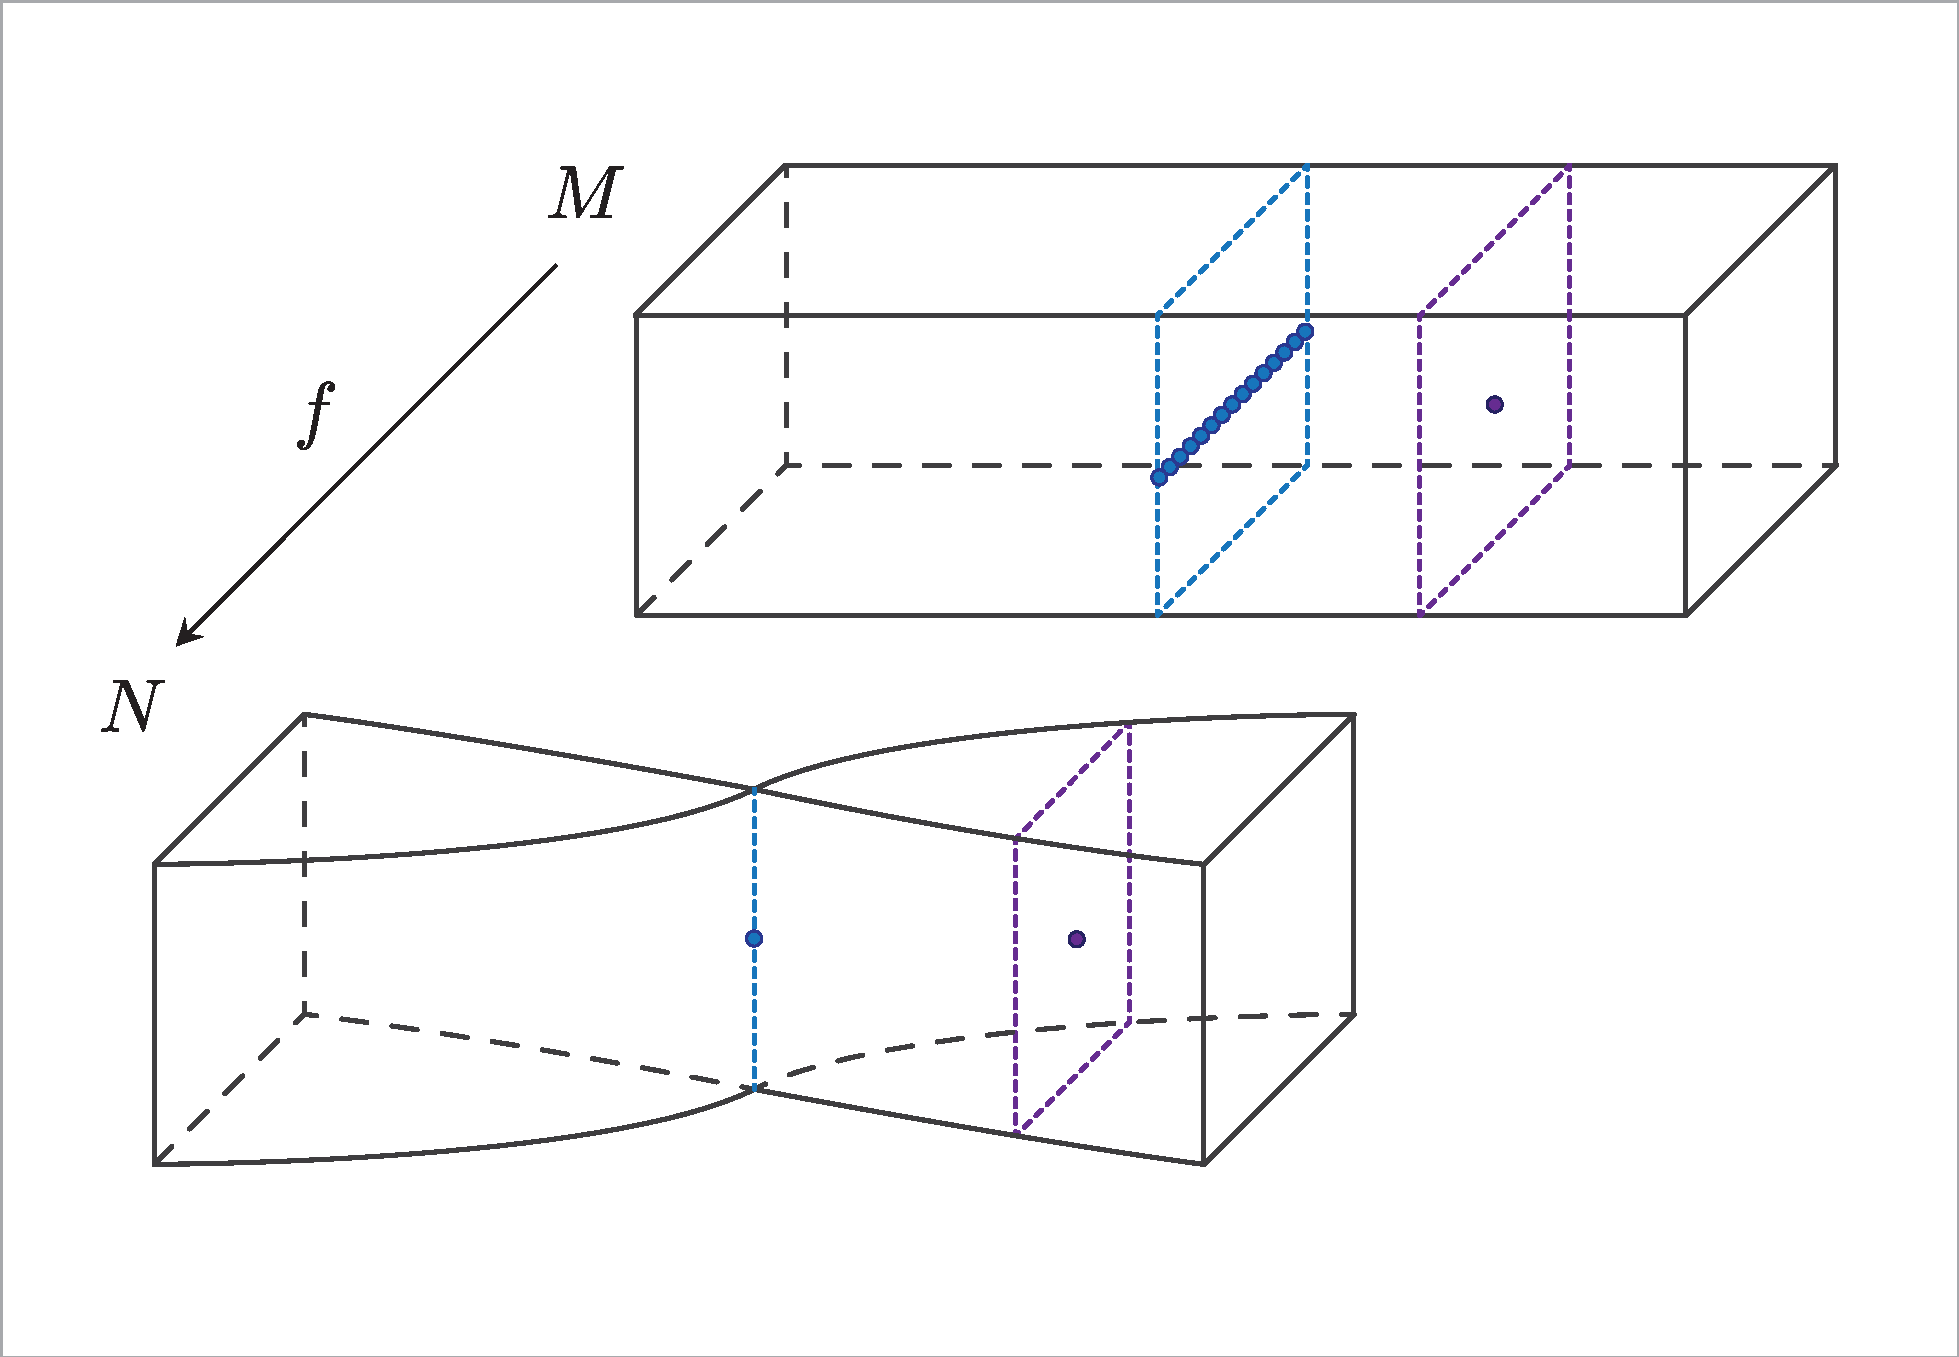
\includegraphics[width=0.85\textwidth]{Degeneracy2.pdf}
			\caption{An example of degeneration of a morphism between varieties }
		\end{figure}
	\end{comment}
	In our case we work in a more general setting: we consider a morphism between two locally free sheaves of finite type, but the underlying intuition is similar.\\

	Let $\ph:E\to F$ be a morphism of locally free sheaves of finite ranks $e$ and $f$ over a Noetherian scheme $Y$ and $n \leq \min(e,f)$. We are interested in studying the $(n-1)$-\textbf{degeneracy locus} of $\ph$, which is defined as
	$$ D_{n-1} (\ph) = \set{ y\in Y \mid \rank_y(\ph) < n }. $$
	Since we want to work with degeneracy loci, it is useful to define the ideal $I_n(\ph)$, generated by all of the $n\times n$ minors of $\ph$. This can be done in a coordinate-free way through the formalism of exterior algebra:
	\begin{defi}
	Let $\ph:E\to F$ be a map of free modules over a ring $R$. We define the ideal $I_n(\ph) \subset R$ to be the image of the canonical map induced by $\ph$ 
	$$ \wedge^n E \otimes\wedge^n F^*\to R. $$
	\end{defi}
	\begin{rema}
		The canonical map involved in the definition of $I_n(\ph)$ is obtained in the following way: first, by the universal property of exterior algebra, given $\nobreak{\ph:E\to F}$ we have a unique map
		$$ \wedge^n\ph : \wedge^n E \to \wedge^n F $$
		and we can thus define the above canonical map as
		$$ \wedge^n E \otimes\wedge^n F^*\to R, \qquad a\otimes b \mapsto b(\wedge^n\ph(a)) $$
	\end{rema}

	Next we introduce the concept of the $n$-th Fitting ideal associated to to a finitely presented module. This is a powerful algebraic invariant, which will serve us to define the moduli varieties \moduu parametrising effective divisors and linear series.

	\begin{defi}
		Let $G$ be a finitely presented module over a ring $R$ and consider a free presentation 
		$$ E \overset{\ph}\to F \to G \to 0 $$ of $G$ such that $F$ is a finitely generated $R$-module of rank $f$. For every integer
		$t \in \N$ we define the $t$-th \textbf{Fitting ideal} of $G$ to be 
		$$ \Fitt_t(G) := I_{f-t}(\ph). $$
	\end{defi}

	\begin{rema}
	Fitting ideals are well-defined, since $\Fitt_t(G)$ does not depend on the chosen presentation. More precisely, if we have another presentation
			$$ E' \overset{\ph'}\to F' \to G \to 0 $$
			with $F'$ of rank $f'$ then $I_{f-t}(\ph) = I_{f'-t}(\ph') $, as it was proved by Hans Fitting in his paper \cite{FITT} of 1936.
	\end{rema}
	The above remark allow us to extend the definition to quasicoherent sheaves over a scheme.
	\begin{defi}
		Let ${G}$ be a locally-free coherent sheaf over a Noetherian scheme $Y$. We have local free presentations of ${G}$ over an open cover of $Y$ and, due to the above remark, the local $t$-th Fitting ideals fit together into a globally defined sheaf of ideals on $Y$, which we denote by $\Fitt_t({G}) \subset \calO_Y$.\\
		Since the ideal sheaf $\Fitt_t({G})$ is coherent by construction, it cuts out a closed subscheme of $Y$ which we denote by $ \FittS_t({G}) $, the $t$-\textbf{Fitting scheme} of ${G}$.
	\end{defi}
	Another useful property of Fitting ideals is their \textbf{invariance under base change}. More precisely, for every morphism of schemes $f:Y'\to Y$, the pullback of the Fitting ideal $f^*\Fitt_t({G})$ is generated as an $\calO_{Y'}$-module by the Fitting ideal of the pullback $\Fitt_t(f^*{G})$.\\
	
	Finally we define the locus of points $y$ where the fibers of $\ph_y$ have a certain dimension:
	\begin{defi}
		Let $m\in \N$ and $\ph:E\to F$ be a morphism of locally free sheaves over a Noetherian scheme $Y$. We define the set
		$$ \Fib_m (\ph) = \set{ y\in Y \mid \text{ fibers of } \ph_y \text{ have dimension } \geq m } $$
	\end{defi}
	Notice that, if $s\in \N$ and we have a free presentation of a coherent sheaf $G$
	$$ E\overset{\ph}\to F \to G\to 0 $$
	with $E$ of rank $e$ and $F$ of rank $f$, then it is a trivial consequence of the definitions that there is the following set-theoretic relationship among the objects we just defined:
	\begin{equation}\label{eq:degeneracy}
		\Supp\left[\,\FittS_{(s-1)}(G)\,\right] = D_{(f-s)}(\ph) = \Fib_{(e-f+s)}(\ph).
	\end{equation}
	

\section{Definition of \modu}\label{sec:defi_modu}
	%
	In order to define $\Xdr$ and $\Wdr$ -- the varieties parametrising linear series -- we will consider the free presentation appearing in Proposition \ref{prop:free_pres}, namely
	$$ 
	\pi_* \calO_{\Delta}(\Delta)\overset{\delta}\tolong R^1 \pi_* \calO \tolong R^1 \pi_* \calO(\Delta) \tolong 0 
	$$
	arising naturally from the universal divisor $\Delta$ and, further, the free presentation
	$$ 
	\nu_{*} \scL(\Gamma)\tolong \nu_{*} \scL(\Gamma) / \scL \tolong R^1 \nu_{*} \scL \tolong 0
	$$
	associated to the universal line bundle $\scL$.
	As we explained in Chapter \ref{chap:relative_Pic_and_Div}, the first of the above presentations -- which lives over $X\times \Dd$ -- is related to the tangent map of the Abel-Jacobi map $u$ and thus embeds information on its degeneracy loci. 
	Further, in Proposition \ref{prop:scheme_theo_inv_img} we will show that the second one -- which lives over $X\times \Pd$ -- encodes basically the same information \emph{modulo linear equivalence} and in fact pulls back to the first one, via $u$. 
	For these reasons we will use the schemes associated to some specific Fitting ideals of these presentations to define \modu.
	\begin{defi}
		We define
		$$ \Xdr := \FittS_{(g-d+r-1)}(R^1\pi_* \calO(\Delta)) \AND  \Wdr := \FittS_{(g-d+r-1)}(R^1\nu_{*} \scL) $$
	\end{defi}
	As a preparation for the next Proposition we need the following Lemma, which illustrates in what precise sense the sequence \eqref{eq:univ_lb_direct_image} associated to the universal divisor is functorial.
	\begin{lemm}\label{lemm:functoriality}
		Let $L$ be a line bundle of degree $d$ on $X\times T$ and let $f:T\to \Pd$ the unique map for which
		$$ f^*\scL \cong L \otimes \phi^* F $$
		where $F$ is a line bundle over $T$ and $\phi: X\times T \to T$ is the natural projection. Further, let $\Gamma':= \phi^* M$ where $M$ is a divisor of high degree $m$ as defined in \ref{def:Gamma}.
		Then the sequence \eqref{eq:univ_lb_direct_image} pulls back via $f$ to the exact sequence
		$$ 0 \to \phi_*L\otimes F  \to \phi_* L(\Gamma')\otimes F \to \phi_* (L(\Gamma') / L)\otimes F  \to R^1 \phi_* L\otimes F  \to 0 $$ 
	\end{lemm}
	\begin{rema}
		Before starting with the proof let us remark that, given a family of line bundles $L$ as in the above statement, we have an exact sequence which is very similar to \eqref{eq:univ_lb_direct_image}. Indeed, since $\Gamma'$ is the pullback of a divisor of high degree on $X$, Lemma \ref{lemm:trivial_R1} of Appendix A implies $R^1\phi_* L(\Gamma') = 0$. Therefore, considering the \ses 
		$$ \SES{L}{L(\Gamma')}{L(\Gamma')/L} $$
		and taking the direct image through $\phi$ we obtain the exact sequence
		$$ 0 \to \phi_*L  \to \phi_* L(\Gamma') \to \phi_* (L(\Gamma') / L)  \to R^1 \phi_* L  \to 0\;. $$
	\end{rema}
	\begin{proof}
		First of all we notice that the locally free sheaf $\scL(\Gamma)$ enjoys the following properties 
		\begin{itemize}
			\item $\nu_{*} \scL(\Gamma)$ is locally free, as showed in Proposition \ref{prop:free_pres}
			\item $R^i \nu_{*} \scL(\Gamma) = 0$ for every $i\geq 1$, as proven in Lemma \ref{lemm:trivial_R1}
		\end{itemize}
		Hence we can apply Proposition \ref{prop:R1_trick} of Appendix A to the base change diagram
		$$
		\begin{tikzpicture}[node distance=5em, auto]
			\node (A) 															{$X\times T$};
			\node (B) 	[right of=A, xshift=4em]		{$X\times \Pd$};
		  \node (C) 	[below of=A]	 							{$T$};
		  \node (D) 	[below of=B] 								{$\Pd$};
		  \draw[-stealth] 				(A)		to node {$1\times f$} (B);
		  \draw[-stealth]					(C)		to node {$f$} 				(D);
		  \draw[-stealth][swap]		(A)		to node {$\phi$} 			(C);
		  \draw[-stealth]					(B)		to node {$\nu$} 			(D);
		\end{tikzpicture}
		$$
		and, using the Projection Formula \eqref{eq:proj_formula}, we deduce that there is a natural isomorphism
		\begin{equation}
			f^* R^1 \nu_{*} \scL(\Gamma) \cong  R^1 \pi_* f^* \scL(\Gamma) \cong R^1 \pi_* (L(\Gamma')\otimes \phi^*F ) \cong R^1 \pi_* L(\Gamma') \otimes F \,.
		\end{equation}
		Moreover, during the proof of Proposition \ref{prop:free_pres} we showed that $\nu_{*} \scL(\Gamma)/\scL $ is also locally free and, further, from the exactness of the direct image sequence
		$$ 
			\dots \to R^1 \nu_{*} \scL \to 0 \to R^1 \nu_{*} \scL(\Gamma)/\scL \to 0 \to \dots
		$$
		we see that $R^i \nu_{*} \scL(\Gamma)/\scL = 0$ for every $i\geq 1$ and, therefore, another application of Proposition \ref{prop:R1_trick} together with the projection formula gives us the natural isomorphism
		$$
			f^* R^1 \nu_{*} \scL(\Gamma)/\scL \; \cong \;  R^1 \pi_* L(\Gamma')/L \otimes F \,.
		$$
		As a result, recalling that \emph{tensoring with a line bundle} is an exact functor, we get the commutative diagram
		$$
		\begin{tikzpicture}[node distance=8em, auto]
			\node (O) 																{$0$};
			\node (A) 	[right of=O, xshift=-4em]			{$f^* (\nu_{*}\scL)$};
			%node (A2) 	[right of=A]									{$\;$};
			\node (B) 	[right of=A, xshift=-1em]			{$f^* (\nu_{*} \scL(\Gamma))$};
			%node (B2) 	[right of=B]									{$\;$};
		  \node (C) 	[right of=B, xshift=1.5em] 		{$f^* (\nu_{*} \scL(\Gamma)/\scL)$};
			%\node (C2) 	[right of=C]						 		{$\;$};
		  \node (D) 	[right of=C, xshift=1em] 			{$f^* (R^1 \nu_{*} \scL)$};
			\node (OO) 	[right of=D, xshift=-3.5em] 	{$0$};
		  \node (O') 	[below of=O,  yshift=3em] 		{$0$};
		  \node (A') 	[below of=A,  yshift=3em] 		{$\phi_*L\otimes F$};
		  \node (B') 	[below of=B,  yshift=3em] 		{$\phi_* L(\Gamma')\otimes F$};
		  \node (C') 	[below of=C,  yshift=3em] 		{$\phi_* (L(\Gamma') / L)\otimes F$};
		  \node (D') 	[below of=D,  yshift=3em] 		{$R^1 \phi_* L\otimes F$};
			\node (OO') [below of=OO, yshift=3em] 		{$0$};
			%
			\draw[-stealth] 					(O)		to node {} 				(A);
		  \draw[-stealth]						(A)		to node {} 				(B);
		  \draw[-stealth]						(B)		to node {} 				(C);
		  \draw[-stealth]						(C)		to node {} 				(D);
			\draw[-stealth]						(D)		to node {} 				(OO);
			\draw[-stealth] 					(O')	to node {} 				(A');
		  \draw[-stealth]						(A')	to node {} 				(B');
		  \draw[-stealth]						(B')	to node {} 				(C');
		  \draw[-stealth]						(C')	to node {} 				(D');
			\draw[-stealth]						(D')	to node {} 				(OO');		  
		  \draw[-stealth][dashed]		(A)		to node {} 				(A');
			\draw[-stealth]						(B)		to node {$\cong$} (B');
		  \draw[-stealth]						(C)		to node {$\cong$} (C');
		  \draw[-stealth][dashed]		(D)		to node {} 				(D');
		\end{tikzpicture}
		\vspace{0em}
		$$
		where of course the dashed arrows are also isomorphisms.
	\end{proof}
	For future reference, we remark the following obvious consequence of the above Lemma.
	\begin{coro}\label{coro:functoriality}
		In the situation of the above Lemma, we have a natural isomorphism
		$$ f^* R^1 \nu_{*} \scL \;\cong\;  R^1 \phi_* L \otimes F $$
	\end{coro}
	The following proposition will clarify the relationship between $\Xdr$ and $\Wdr$, showing that $\Xdr$ is the scheme-theoretical inverse image of $\Wdr$. 
	\begin{prop}\label{prop:scheme_theo_inv_img}
		The scheme theoretic inverse image of the variety $\Wdr$ via the Abel-Jacobi map equals $\Xdr$. In symbols this amounts to
		$$ u^{-1}(\Wdr) = \Xdr. $$
	\end{prop}
	\begin{proof}
		We remarked already that Fitting ideals are stable under base change and this implies in particular that, for any sheaf $\scr{F}$, $u^*\Fitt(\scr{F})$ is generated as a module by $\Fitt(u^*\scr{F})$. Therefore the ideal sheaf of $u^{-1}(\Wdr)$ is generated by $\Fitt(u^* R^1\nu_{*}\scL)$ and thus it is enough to show that the latter is isomorphic to $\Fitt(R^1\pi_* \calO(\Delta))$. To begin, pick $D\in \Dd$ and notice that the canonical maps
		$$ f: D \into \Dd \AND g: \calO(D)\into \Pd $$
		satisfy the relation $g = u\circ f$. So fiberwise we have the identities
		$$ (u^* \scL)_{\mid D} = f^* u^* \scL = (u\circ f)^* \scL = g^* \scL = \calO(D) = \calO(f^* \Delta) = f^*\calO(\Delta) = \calO(\Delta)_{\mid D} $$
		and we can therefore apply Lemma \ref{lemm:square} of Appendix A to get a line bundle $F$ over $\Dd$ such that
		$$ u^* \scL \;\cong\; \calO(\Delta) \otimes \pi^* F \,, $$
		where $\pi: X\times \Dd \to \Dd$ is the natural projection map. Finally, from Corollary \ref{coro:functoriality} we get a natural isomorphism
		$$ u^*  R^1\nu_{*}\scL \;\cong\; R^1\pi_*\calO(\Delta)\otimes F $$
		and, since $\square\otimes F$ is a right-exact functor and does not affect Fitting ideals, we therefore conclude that
		$$ \Fitt(u^* R^1\nu_{*}\scL) 
		\;\cong\; 
		\Fitt(R^1\pi_*\calO(\Delta))\,, $$
		as desired.
	\end{proof}


	We will now show that the support of $\Xdr$ consists of divisors with rank at least $r$. To start, recall from Proposition \ref{prop:free_pres} that the terms appearing in (\ref{eq:univ_div_seq}) are locally free sheaves over $\Dd$, and the first two have rank respectively $d$ and $g$, so that with respect to the notation used in the identities \eqref{eq:degeneracy} we have 
	\begin{equation}\label{eq:e_f_k}
		e=d, \qquad f=g \AND s=g-d+r.
	\end{equation}
	Moreover from Proposition \ref{prop:delta_u} we know that we can identify $\delta$ with $\Tu$ and thus, exploiting the above mentioned identities , we find
	\begin{equation*}
		\Supp(\Xdr) = \Fib_{(r)}(\Tu) = \set{ D\in \Dd \mid r(D) \geq r }.
	\end{equation*}
	\begin{comment}
		\begin{eqnarray*}
			\Supp(\Xdr) 
			&=& \Supp\scr{Z}(I_{g-(g-d+r-1)}\delta) \\
			&=& \Supp\scr{Z}(I_{(d-r+1)}\delta) \\
			&=& \set{ D\in \Dd \mid \rank_D(\delta) \leq d-r } \\
			&=& \set{ D\in \Dd \mid \rank_D(\Tu) \leq d-r } \\
			&=& \set{ D\in \Dd \mid \text{the fibers of } \TDu \text{ have dimension } \geq r } \\
			&=& \set{ D\in \Dd \mid r(D) \geq r }.
		\end{eqnarray*}
	\end{comment}
	Since from Proposition \ref{prop:scheme_theo_inv_img} it follows in particular that $u$ maps $\Xdr$ onto $\Wdr$, we therefore immediately see that the support of $\Wdr$ is given by 
	$$ \Supp(\Wdr) = \set{ L \in \Pd \mid r(L) \geq r } $$


	\begin{figure}[ht]
		\centering
		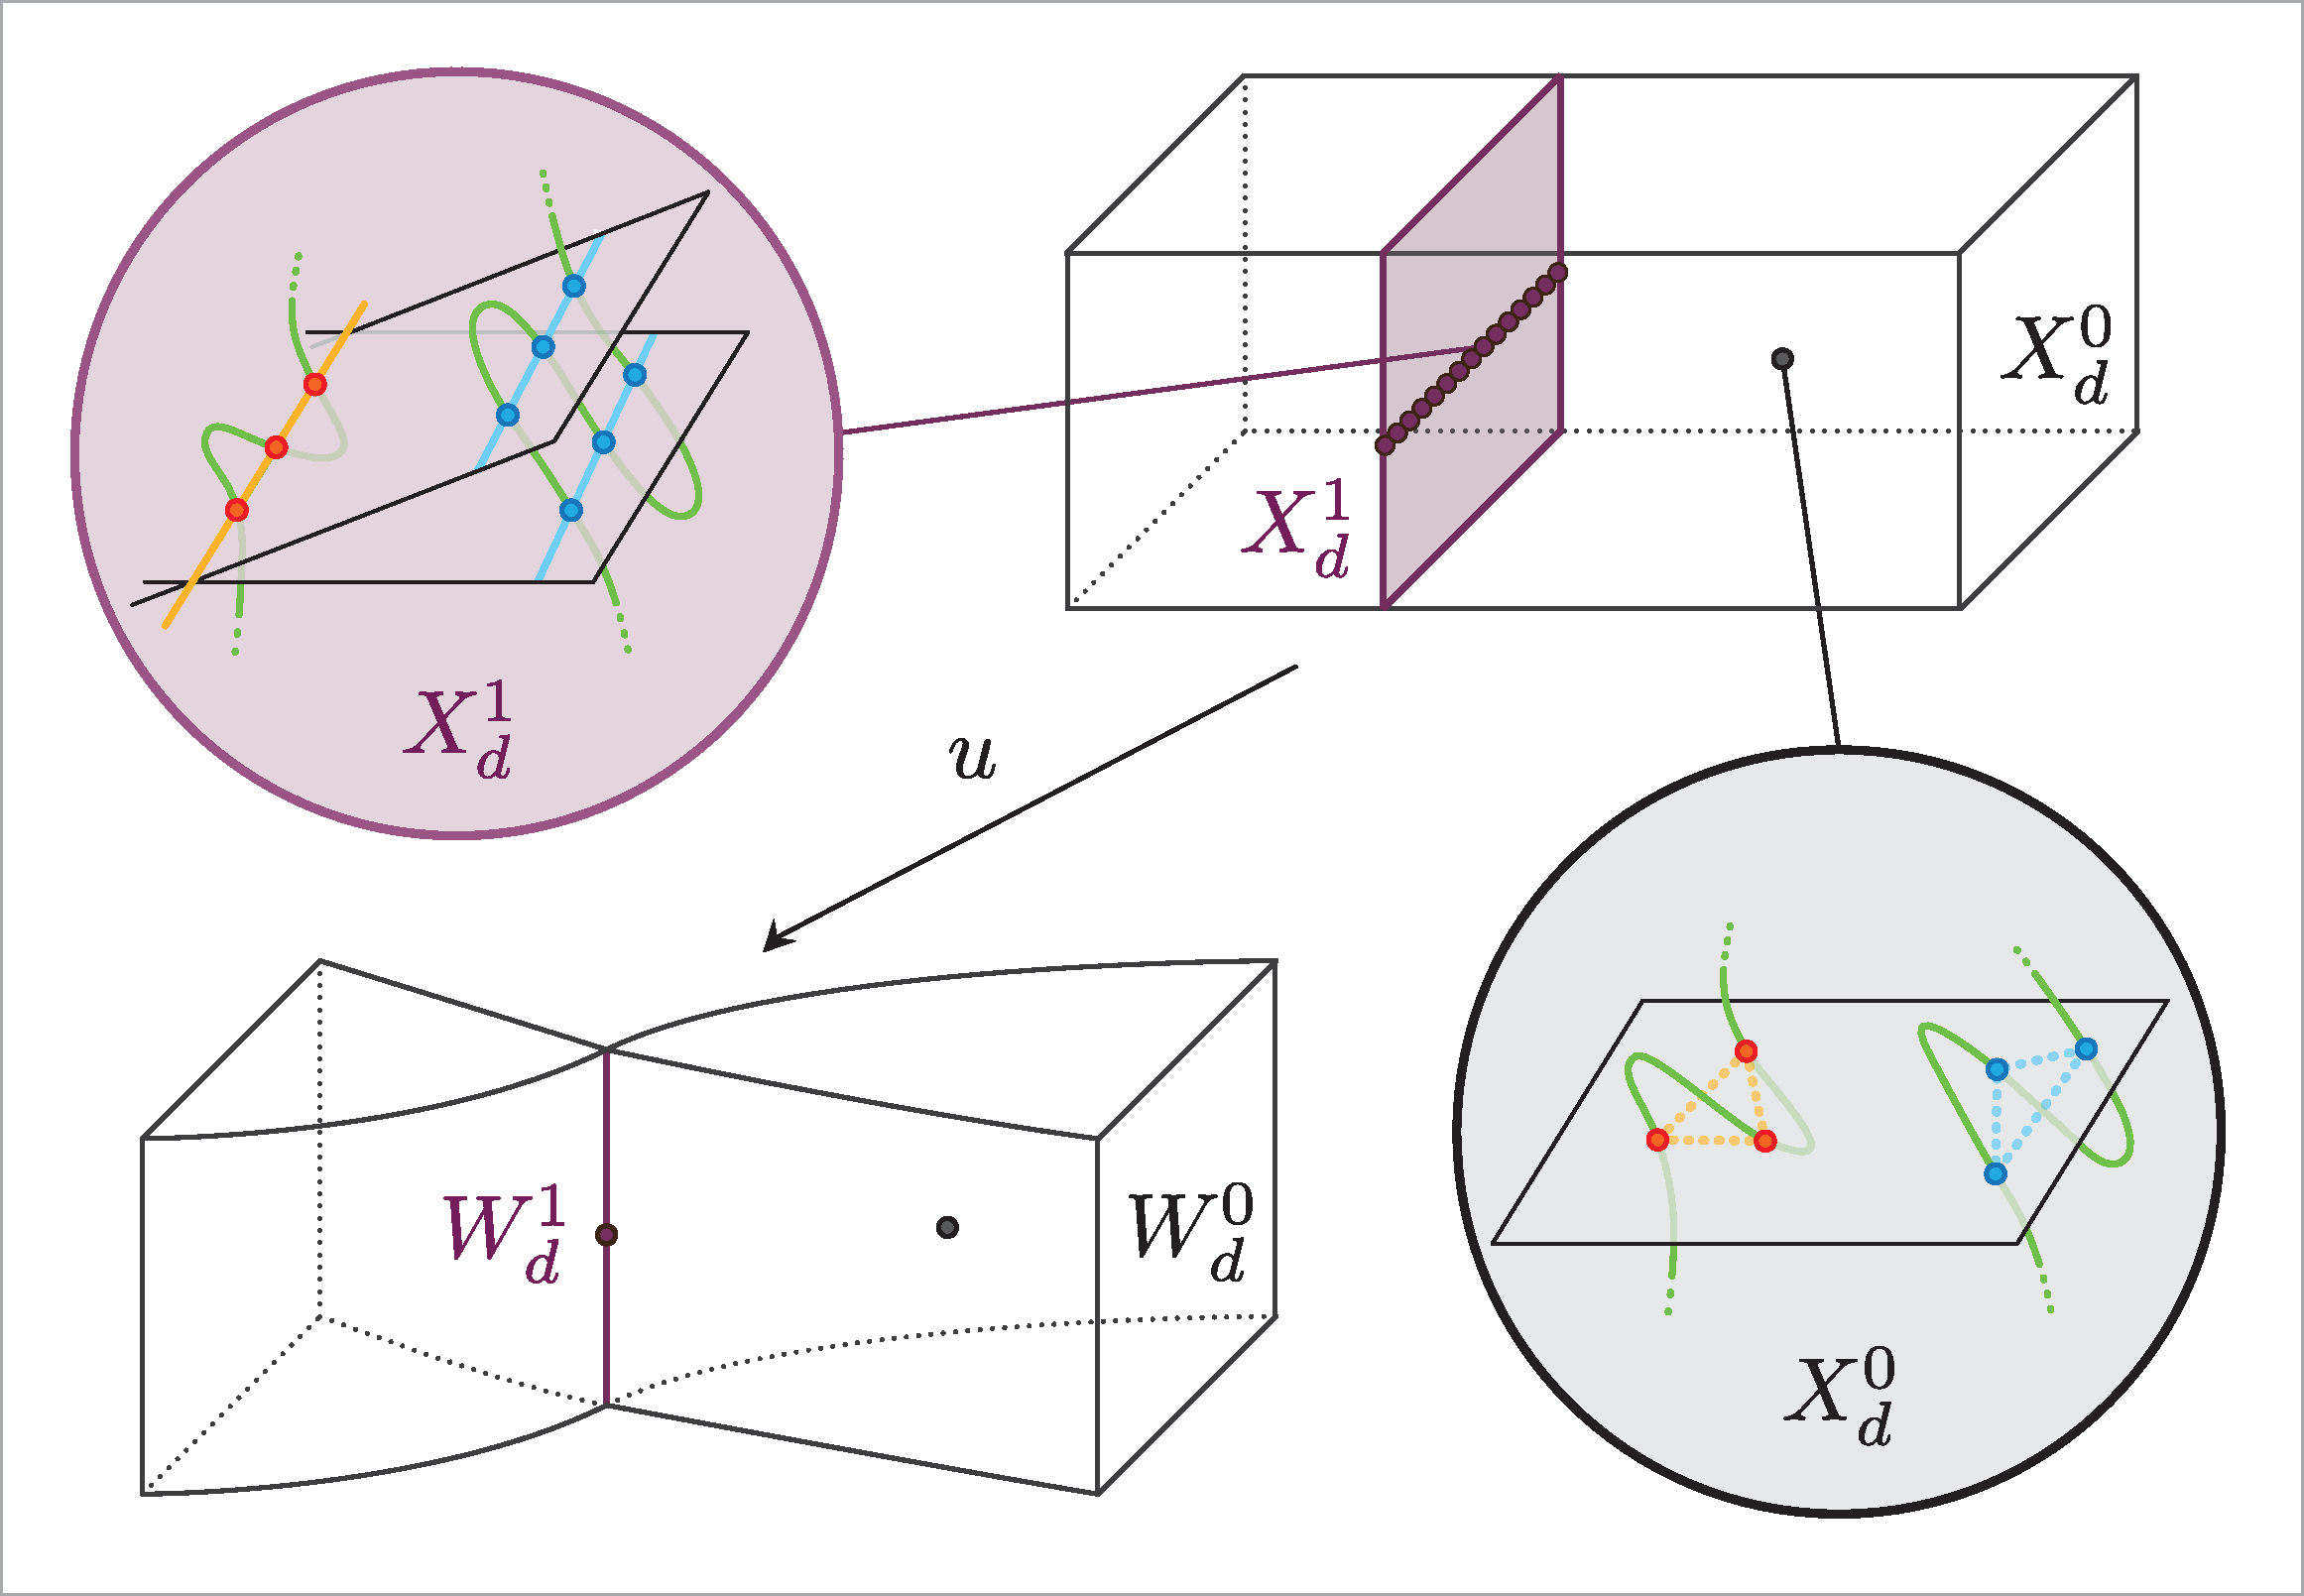
\includegraphics[width=\textwidth]{Degeneracy3.pdf}
		\caption{An intuitive picture of the Degeneracy loci of the Abel-Jacobi map $u$.}
	\end{figure}


\section{Dimensional lower bounds}\label{sec:lower_bound}
	%
	First of all let us introduce to the reader the so called \BN number, which will turn to be a crucial ingredient of \BN theory.
	\begin{defi}
		Let $d$, $g$ and $r$ be natural numbers. The \textbf{Brill-Noether number} is defined as
		$$\rho = \rho(d,g,r) = g - (r+1)(g-d+r)$$
	\end{defi}
	\vspace{1em}
	Let now $G$ be a finitely presented sheaf which admits the free presentation
	$$ E\overset{\ph}\to F \to G\to 0 $$
	with $E$ of rank $e$ and $F$ of rank $f$. Applying Theorem \ref{thm:height} of Appendix A to $G$ we get
	$$ \height (\Fitt_t(G)) \leq (e-f+t+1)(t+1). $$
	In the case of $\Xdr$, the sheaves appearing in the presentation \eqref{eq:univ_div_seq} have rank $d$ and $g$ as in \eqref{eq:e_f_k}. Hence, denoting by $I$ the (Fitting) ideal sheaf of $\Xdr$ we have
	$$ \height (I) \leq r(g-d+r). $$
	Since $\Dd$ is a variety over a field, it is a catenary scheme and we have the equality $ \codim \Xdr + \dim \Xdr = \dim \Dd $. Thus, recalling that $\dim \Dd = d$ we get the lower bound
	$$ \dim \Xdr \geq d - r(g-d+r) = g-(r+1)(g-d+r) + r = \rho + r $$
	for the dimension of every irreducible component of  $\Xdr$. Further, invoking Proposition \ref{prop:scheme_theo_inv_img} we deduce that any irreducible component of $\Wdr$ has dimension greater or equal than $\rho $. Let us state these results in the form of a Theorem, for future reference
	\begin{theo}\label{thm:lowerbounds}
		Every irreducible component of $\Xdr$ has dimension at least $ \rho + r$, while every irreducible component of $\Wdr$ has dimension at least $ \rho $.
	\end{theo}


\section{Definition of $\Gdr$}

	We are now going to define a variety $\Gdr$ parametrising $g_d^r$ on the curve $X$, i.e.\ (not necessarily complete) linear series of degree $d$ and dimension $r$. Our objective is to give the right definition for $\Gdr$ and then show that its support is given by
	$$ \Supp(\Gdr) = \set{ (L,W) \in \Pd \times \mathbb{G}(r+1, H^0(L)) } $$
	where $L$ is a line bundle on $X$ and $\mathbb{G}(r+1, H^0(L))$ denotes the Grassanian bundle of $(r+1)$-dimensional linear subspaces of $H^0(L)$.
	In order to give a scheme structure to $\Gdr$, we need to introduce a useful algebraic object. Let $G$ be a locally free and finitely presented sheaf over a scheme $Y$ and $ E\overset{\varphi}\to F \to G \to 0$ a free presentation of $G$, where $E$ and $F$ have finite ranks $e$ and $f$. Moreover, for every natural number $t\leq e$, let
	$$ \pi:\mathbb{G}(e-t, E)\to Y $$ 
	be the projection from the Grassmannian bundle of $(e-t)$-subspaces of sections of $E$ to $Y$.
	Consider the natural short exact sequence of sheaves over $\mathbb{G}(e-t, E)$
	$$ 0\to S \to \pi^* E \to Q \to 0 $$
	where $S$ and $Q$ are the universal subbundle and quotient bundle of $\mathbb{G}(e-t, E)$. 
	In order to better understand this sequence, let $y\in Y$ and let the $(e-t)$-subspace $V=\pi^{1}(y)$ be the corresponding fiber over $y$. Then the fiberwise \ses over $V$ is simply given by
	$$ 0\to V \to E_y \to E_y/V \to 0 \,. $$
	Next, we define the following subset of $\mathbb{G}(e-t, E)$ as a specific vanishing locus:
	\begin{defi}
		Ve define $\Grass_t(G) \subset \mathbb{G}(e-t, E)$ to be the vanishing locus of the morphism of sheaves
		$$ S\longrightarrow \pi^*E \overset{\pi^*\varphi} \longrightarrow \pi^* F $$
		i.e.\ the closed subset of the support of $\mathbb{G}(e-t, E)$ consisting of those points over which $S\to \pi^* F$ restricts to the zero morphism.
	\end{defi}
	\begin{rema}\label{rema:ker}
		Notice that, by definition, the support of $\Grass_t(G)$ consists of pairs $(y, V)$ where $y\in Y$ and $V\subset E_y$ is a $(e-t)$-subspace contained in the kernel of the linear map $\ph_y: E_y \to F_y$.
	\end{rema}
	Hence we can use the notion of $\Grass_t(\bullet)$ to define the variety $\Gdr$. To do so, first recall the definition of the high-degree divisor $\Gamma$ of degree $m$ as in Definition \ref{def:Gamma} and then consider the free presentation \eqref{eq:univ_lb_seq} of finite rank locally free sheaves over $\Pd$
	$$ \nu_{*} \scL(\Gamma)\overset{\gamma}\to R^1 \nu_{*} \scL(\Gamma) / \scL \to R^1 \nu_{*} \scL \to 0 $$
	which was involved in the definition of $\Wdr$.
	\begin{defi}
		We define $\Gdr$ to be the closed subscheme of $\mathbb{G}(r+1, \nu_{*} \scL(\Gamma))$ given by $\Grass_{(d+m-g+r)}(R^1 \nu_{*} \scL)$.
	\end{defi}
	One can show that the above definition is independent from the choice of the presentation of $R^1 \nu_{*} \scL$. We do not deal with this problem and we leave it as an exercise to the interested reader.\\

	It is now time to check that $\Gdr$ actually parametrizes $g_d^r$ on the curve. 
	First of all observe that, by Lemma \ref{lemm:functoriality}, the kernel of $\gamma_{\mid L}$ over any $L \in \Pd$ is canonically isomorphic to $H^0(L)$. 
	Therefore, looking at Remark \ref{rema:ker}, we see that the support of $\Gdr$ consists of couples $(L, W)$ where $L$ is a line bundle of degree $d$ and $W\subset H^0(L)$ is a linear subspace of dimension $r+1$, as desired.


\section{Cohomological description for the tangent spaces}

	In the following we will use the short hand notations
	$$ \Xdrr = \Xdr\setminus X_d^{r+1} \AND \Wdrr = \Wdr\setminus W_d^{r+1} $$
	and we will refer to the points of $\Xdrr$ and $\Wdrr$ as \textbf{good points}.\\
	With the aim of describing the tangent space of $\Wdr$ and $\Xdr$, we will first look at the one of $\Gdr$. A motivation for this approach is the observation that the natural projection
	$$ \beta:\Gdr\to\Wdr, \qquad (L,W) \mapsto L $$
	is biregular away of $W_d^{r+1}$. Indeed $\beta$ is clearly a regular map and, further, the preimage of $L\in \Wdrr$ consists just of the point $w=(L,H^0(L))$. It follows that, as far as $\Wdrr$ is regarded, $T\beta$ gives an isomorphism between the tangent spaces
	\begin{equation}\label{eq:tgnt_Wdrr}
		T\beta : T_{w}\Gdr \toiso T_L\Wdr, \quad \forall L\in\Wdrr.
	\end{equation}
	In order to describe the tangent space of $\Gdr$, a preliminary result about the first order deformations of a pair $(L,s) \in \Pic^d \times H^0(L)$ will turn out to be crucial.
	\begin{prop}\label{prop:cohom_condition}
		Let $L\in \Pic^d$ be a line bundle over $X$ and $s\in H^0(L)$ a global section. Then an element $\phi \in T_L\Pic^d \cong H^1(\OX)$ induces a first order deformation of the pair $(L,s)$ \ABiff $\phi\cdot s=0$ in $H^1(L)$.
	\end{prop}
	\begin{proof}
		Assume that $L$ is given by transition functions $g_\alb$ on a open cover $U_\al$ of $X$. We already know that $T_L \Pic^d \cong H^1(\OX)$ and a first order deformation $L'$ of $L$ is represented by a class $\phi \in H^1(\OX)$ in the following way
		$$ g_\alb \quad\overset{\phi}\leadsto\quad g'_\alb = g_\alb \cdot (1+ \eps \phi_\alb). $$  
		On the other hand, on a first order deformation of the pair $(L,s)$ to $(L',s')$ we have the additional requirement that the section $s'$ corresponds to a linear deformation of $s$. In formula this is expressed as
		$$ s'_\al = s_\al + \eps t_\al, \quad t \in H^0(L). $$
		The action of the transition functions can therefore be expanded as
		$$ s'_\beta = g'_\alb \cdot s'_\al \;\iff\; s_\beta + \eps t_\beta = g_\alb \cdot (1 + \eps \phi_\alb)\cdot(s_\al + \eps t_\al)$$
		and imposes the conditions
		$$ s_\beta = g_\alb \cdot s_\al \AND \phi_\alb \cdot s_\al = t_\al - g_{\beta\al}\cdot t_\beta. $$
		The first one is automatically satisfied since $s$ is a global section of $L$, while the second one can be rewritten in terms of the coboundary map $\partial : C^0(L) \to C^1(L)$ as
		$$ \phi \cdot s = \partial (t), $$
		thus giving the desired result.
	\end{proof}
	We now have a way to describe an element of $T_w\Gdr$. In fact the latter is nothing but a first order deformation of the pair $(L,W)$ and, as an immediate consequence of the above Proposition, one such deformation corresponds to an element $\phi\in H^1(\OX)$ such that $\phi\cdot W = 0$. Hence we deduce that the image of $T\beta$ at a point $w=(L,W)$ can be described as
	\begin{equation*}
		T\beta(T_w \Gdr) \cong \set{ \phi \in H^1(\OX) \mid \phi\cdot W = 0 \text{ in } H^1(L) }.
	\end{equation*}
	Further, this description can be reformulated using Serre's duality by considering the restriction of $\mu_0$ to $W\subseteq H^0(L)$, i.e.\ the map
	$$ \mu_{0,W} : W\otimes H^0(K-L) \to H^0(K), \quad s\otimes s' \mapsto s\cdot s'. $$
	Indeed, since the duality pairing is perfect, the condition $\phi\cdot W = 0$ is equivalent to require that $\forall s\in W$ and $\forall s'\in H^0(K-L)$ the pairing
	$$ \langle\, s',\, s\cdot \phi \, \rangle = \langle \,s'\cdot s,\, \phi \,\rangle $$
	vanishes. Notice that the above identity follows from Lemma \ref{lemm:pairing_properties} of Appendix A and the local description of abelian differentials. Therefore, in a more concise form, we can write 
	\begin{equation}\label{eq:im_beta_*}
		T\beta(T_w \Gdr)\cong(\,\im \mu_{0,W}\,)^{\vee}.
	\end{equation}

	As a consequence, at least for good points, we can easily describe the tangent space of $\Wdr$ in a purely cohomological fashion.
	\begin{prop}\label{prop:tgnt_Wdr}
		For every good point $L\in \Wdrr$ the tangent space is given by
		$$ T_L\Wdr \cong (\,\im \mu_{0}\,)^{\vee} $$
		where $ \mu_{0} : H^0(L)\otimes H^0(K-L) \to H^0(K) $ is the cup product.
	\end{prop}
	\begin{proof}
		This follows immediately from \eqref{eq:tgnt_Wdrr} and \eqref{eq:im_beta_*}, taking $W=H^0(L)$.\\
	\end{proof}
	Exploiting the fact that $\al$ is dual to $\delta$ we get, as a corollary, a nice cohomological description for the tangent space of $\Xdr$ as well.
	\begin{coro}\label{coro:tgnt_Xdr}
		For every good point $D\in \Xdrr$ the tangent space is given by
		$$ T_D\Xdr \cong (\,\im \al \mu_{0}\,)^{\vee} $$
		where $ \mu_{0} : H^0(D)\otimes H^0(K-D) \to H^0(K) $ is the cup product.
	\end{coro}
	\begin{proof}
		Let $D \in \Xdrr$ and set $L=u(D)$. Using Proposition \ref{prop:tgnt_Wdr} we find
		\begin{eqnarray*}
			T_D \Xdr 
			&=& u_{*}^{-1}\; T_L \Wdr \\
			&=& u_{*}^{-1}\: (\,\im \mu_0\,)^{\vee} \\
			&=& \delta^{-1}\; (\,\im \mu_0\,)^{\vee} \\
			&=& (\,\im \al \mu_0\,)^{\vee}
		\end{eqnarray*}
		where the last equality holds because $\al$ is dual to $\delta$, as shown in Appendix B -- see identity \eqref{eq:deltalpha}.
	\end{proof}


\section{Consequences of the infinitesimal study}

	The results achieved in this Section shade light on the crucial role of the cup-product homomorphism $\mu_0$ in the study of the geometry of linear series. Indeed, as we will see in the following, the moduli varieties parametrizing effective divisors and linear series present singularities on those points over which the cup-product presents a non trivial kernel. This is a fact which was already observed in the toy-model examples of Section \ref{sec:examples}.
	\\

	We start with a proposition about the dimension of $\Gdr$. 
	\begin{prop}\label{prop:inf_Gdr}
		The dimension of $\Gdr$ is at least $\rho$ and, at every point $w=(L,W)$,  
		$$ \dim T_w \Gdr = \rho + \dim( \ker \mu_{0,W} ) .$$ 
		Hence $\Gdr$ is smooth of dimension $\rho$ at $w$ \ABiff $\mu_{0,W}$ is injective.
	\end{prop}
	\begin{proof}
		The lower bound on the dimension of $\Gdr$ follows directly from Theorem \ref{thm:lowerbounds}, since $\beta$ is onto $\Wdr$. To get the dimension of $T_w \Gdr$, notice that the fiber of $\beta$ over a point $L\in \Wdr$ is canonically isomorphic to the grassmanian $\mathbb{G}(r+1,H^0(L))$, whose tangent space at a point $W$ is given by $\Hom(W, H^0(L) / W)$. Hence we have a \ses
		$$ \SES{ \Hom(W, H^0(L) / W) }{ T_w \Gdr }{ \im (T\beta) } $$
		and the result follows from a trivial computation:
		\begin{eqnarray*}
			\dim T_w \Gdr
			&=& \dim\im(T\beta) + \dim\Hom(W, H^0(L) / W) \\
			&=& g-\dim\im\mu_{0,W} + (r+1)(h^0(L)-r-1) \\
			&=& g-(r+1)h^0(K-L) +\dim(\ker\mu_{0,W}) + (r+1)(h^0(L)-r-1) \\
			&=& g-(r+1)(h^0(K-L) - h^0(L)+r+1) +\dim(\ker\mu_{0,W}) \\
			&=& g-(r+1)(g-d+r) +\dim(\ker\mu_{0,W}) \\
			&=& \rho +\dim(\ker\mu_{0,W})
		\end{eqnarray*}
		The statement about the smoothness now follows immediately.
	\end{proof}
	As a corollary, we get an important result about the dimension and smoothness of $\Wdr$ at good points $L\in \Wdrr$.
	\begin{coro}
		The variety $\Wdr$ is smooth of dimension $\rho$ at $L\in \Wdrr$ \ABiff the cup product $ \mu_{0} : H^0(L)\otimes H^0(K-L) \to H^0(K) $ is injective.
	\end{coro}
	\begin{proof}
		From Proposition \ref{prop:inf_Gdr} together with \eqref{eq:tgnt_Wdrr} we know that for every good point $L$ 
		$$ \dim T_L \Wdr = \rho +\dim(\ker\mu_0) $$
		so it is enough to invoke the lower bound of Theorem \ref{thm:lowerbounds} to conclude.
	\end{proof}
	Finally, we have the corresponding result on the dimension and smoothness of $\Xdr$.
	\begin{prop}
		The variety $\Xdr$ is smooth of dimension $\rho+r$ at $D\in \Xdrr$ \ABiff the cup product $ \mu_{0} : H^0(D)\otimes H^0(K-D) \to H^0(K) $ is injective.
	\end{prop}
	\begin{proof}
		This is another a trivial computation. Indeed, using Corollary \ref{coro:tgnt_Xdr} and noticing that $\ker\al=H^0(K-D)$ is contained in the image of $\mu_0$, we get
			\begin{eqnarray*}
				\dim T_D \Xdr 
				&=& d - \dim\im\al\mu_0 = d - \dim\im\mu_0 + \dim\ker\al \\
				&=& d - (r+1)(g-d+r) + \dim\ker\mu_0  + g-d+r \\
				&=& r + g - (r+1)(g-d+r) + \dim\ker\mu_0 \\ 
				&=& r + \rho + \dim\ker\mu_0.
			\end{eqnarray*}
			The remark about the smoothness of $\Xdr$ at $D$ follows from the above combined with the lower bound of Theorem \ref{thm:lowerbounds}.
	\end{proof}

	These results make it natural to ask how the tangent spaces of the moduli varieties behave in the case of a general curve. An answer is given by a classical result due to Gieseker, which was proved during the last decades for the case of curves over $\C$. 
	\begin{namedtheo}[Smoothness Theorem]
		Let $X$ be a general curve of genus $g$ and let $d\geq 1$, $r\geq 0$ be natural numbers. Then $\Gdr$ is smooth of dimension $\rho$.
	\end{namedtheo} 
	An extension of this Theorem to an arbitrary algebraically closed field is out of the scope of this Thesis, nevertheless the above achieved results strongly suggest that such a generalization is possible.\\
	Because of the cohomological description of the infinitesimal structure of the moduli varieties, the Smoothness Theorem can also be stated in an equivalent and purely cohomological manner:
	\begin{namedtheo}[Smoothness Theorem 2]
		Let $X$ be a general curve of genus $g$ and $D$ and effective divisor on $X$. Then the cup-product homomorphism
		$$ \mu_{0} : H^0(D)\otimes H^0(K-D) \to H^0(K) $$
		is injective.
	\end{namedtheo}


	\begin{comment}
		It would nice to show that at \textbf{bad} points the tangent cones are given by
		$$ T_D\Xdr \cong T_D\Dd \AND T_L\Wdr \cong T_L\Pd $$
		even if, most likely, time will not permit.
	\end{comment}
	






% this file is called up by thesis.tex
% content in this file will be fed into the main document

%: ----------------------- name of chapter  -------------------------
\chapter{Existence and Connectedness Theorems} % top level followed by section, subsection


%: ----------------------- paths to graphics ------------------------

% change according to folder and file names
\ifpdf
    \graphicspath{{figures/}{figures/}{figures/}}
\else
    \graphicspath{{figures/}{figures/}}
\fi

%: ----------------------- contents from here ------------------------


The scope of this Chapter is to achieve a generalization of two basic results of the classical \BN Theory, the Existence and Connectedness Theorems, to the case of an arbitrary algebraically closed field. The content of the Theorems underlines the crucial role of the \BN number $\rho$ in the study of linear series: in fact, a non negative value of $\rho$ implies that $\Wdr$ is not empty and, moreover, $\rho>0$ ensures its connectedness.
These results were proved in the last decades for curves over the complex numbers but, as we will see, can be extended to closed fields of positive characteristic.\\
Thanks to a general result on degeneracy loci proved by Fulton -- Theorem \ref{theo:alg} of Appendix A -- the Existence and Connectedness Theorems will follow immediately, but first we need to show that Fulton's hypothesis are met in our situation. The first step is to show that $\Wdr$ can be seen as a degeneracy locus of a morphism of vector bundles
$$ \ph: E\tolong F $$
where $E$ and $F$ arise from a specific cohomology sequence associated to the universal line bundle $\scL$. It is crucial to choose these vector bundles in a smart way, in order to simplify the following and last step, in which we need to show that the tensor product $E^*\otimes F \cong \Hom(E,F)$ is an ample vector bundle.

\section{An alternative perspective on $\Wdr$}\label{sec:alternative}

	\begin{notation}
		For every natural number $d\in \N$, let $M=\sum_{i=1}^m p_i$ be a divisor of high degree $m\geq2g-d-1$ on $X$ and set $n:=m+d$.
	\end{notation}	
	
	To begin, we will give a recipe to construct an explicit universal line bundle $\scL_n$ of degree $n$ which enjoys the characterizing universal property. Because of the uniqueness up to isomorphisms of such an universal object, the explicit recipe given in  this Section is compatible with the non-constructive approach we adopted in the previous Chapters.

	For now and for the rest of the section, choose a closed point $Q\in X$ and define 
	$$ [Q] := \set{ D\in \Dn \mid Q \in \Supp(D) } \subset \Dn $$
	Further, let $\Delta$ be a universal divisor of degree $n$, let $u:\Dn\to\Pn$ the \AJJ map and $\pi:Z=X\times\Dn\to\Dn$ the natural projection. 
	\begin{defi}\label{def:universal_lb}
		We define a universal line bundle $\scL_n \to X\times\Pn$ of degree $n$ by
		$$ \scL_n := (1_X\times u)_*(\calO_Z(\Delta - \pi^* [Q])) $$
	\end{defi}
	Notice that the above pushforward gives in fact a line bundle, the reason being that the \AJJ map $u$ is onto $\Pn$ since $n$ is greater than $2g-1$.
	Moreover, it is easy to check that the resulting line bundle enjoys the universal property of a universal line bundle, but we leave the details to the interested reader. \\

	Recall that the moduli variety $\Wdr$ was defined as a Fitting scheme associated to the sheaf $R^1\nu_{*}\scL_d$, where $\scL_d$ is a universal line bundle of degree $d$. 
	It will be convenient, in this section, to \emph{translate} our point of view and work directly in higher degree. 
	Hence, using the recipe provided by Definition \ref{def:universal_lb}, choose $\scL_n$ to be a universal line bundle of degree $n=d+m$. 
	Further, let $\Gamma = M\times \Pn$ and use the isomorphism
	$$ a:\Pd\toiso\Pn, \qquad L\mapsto L\otimes \calO(M) $$
	to define the universal line bundle $\scL_d$ of degree $d$ as the pull-back of $\scL_n(-\Gamma)$ 
	$$ \scL_d := a^*\scL_n(-\Gamma). $$
	We claim that the image $a(\Wdr)\subset \Pn$ is the closed subscheme $Y$ corresponding to the Fitting ideal $\Fitt_{t}(R^1\nu_{*}\scL_n(-\Gamma)) $ with $t=g-d+r-1$, the reason being that the scheme theoretic preimage $a^{-1}(Y)$ corresponds to the ideal sheaf
	$$ 	a^*\Fitt_{t}(R^1\nu_{*}\scL_n(-\Gamma)) 
	= 	\Fitt_{t}(a^*R^1\nu_{*}\scL_n(-\Gamma)) 
	= 	\Fitt_{t}(R^1\nu_{*} \scL_d)
	$$
	as one sees invoking Corollary \ref{coro:functoriality} and recalling that Fitting ideals -- defined through a free presentation -- are not affected by tensor product.
	Therefore we understand that $\Wdr$ can also be seen as the $(m-g+d-r)$-degeneracy locus of the evaluation map
	$$ E:=\nu_{*} \scL_n \;\longrightarrow\; \nu_{*} (\scL_n / \scL_n(-\Gamma))=:F, $$
	which will turn out to be a convenient point of view, as we will see in the next Section.


\section{Ampleness of $(\nu_{*} \scL)^* \otimes \nu_{*} (\scL/\scL(-\Gamma))$}\label{sec:ampleness}

	We start by exploiting the choice of the vector bundle $F = \nu_{*} (\scL_n / \scL_n(-\Gamma))$, showing that it admits a simple description in the following Lemma. 

	\begin{notation}
		For the rest of this Section we will write $\scL=\scL_n$ to denote the universal line bundle of degree $n$. Further, for any closed point $P\in X$, denote by $\Gamma_P $ the divisor $P \times \Pn \subset X\times \Pn$.
	\end{notation}
	\begin{defi}\label{def:alg_equiv}
		Two line bundles $L_1$ and $L_2$ over a scheme $Y$ are said to be \textbf{algebraically equivalent} if there exist a connected scheme $T$, two closed points $t_1,t_2\in T$ and a line bundle $L$ over $Y\times T$ such that
		$$ L_{\mid Y\times t_1} \cong L_1 \AND L_{\mid Y\times t_2} \cong L_2. $$
	\end{defi}

	\begin{lemm}\label{lemm:alg_trivial}
		If the divisor $M=\sum_{i=1}^m p_i$ is reduced, then $F=\nu_{*} (\scL / \scL(-\Gamma))$ is a direct sum of algebraically trivial line bundles.
	\end{lemm}
	\begin{proof}
		Let $P$ be a closed point of $X$ and notice that $\scL/\scL(-\Gamma_P)$ is just the restriction of $\scL$ to $\Gamma_P$. Therefore, from the natural isomorphism
		$$ \calO_{X\times X_n}(\Delta)\otimes \calO_{\{P\}\times X_n} \cong \calO_{X_n}([P]) $$
		together with the explicit form of the universal line bundle $\scL = (1_X\times u)_*(\calO(\Delta - \pi^* [Q]))$, we deduce that 
		\begin{equation}\label{eq:description}
			\nu_{*} \left(\scL/\scL(-\Gamma_P)\right) \cong u_* \calO_{X_n}([P]-[Q]).
		\end{equation}
		To show that $\nobreak{u_* \calO_{X_n}([P]-[Q])}$ is algebraically equivalent to the trivial bundle, following the notation of Definition \ref{def:alg_equiv} we can take $L=\scL$, $T=X$ and $t_1=P$, $t_2=Q$ for the points. Indeed one can easily see that we have
		$$ \scL_{\mid \Pn\times \{P\}} \cong u_* \calO_{X_n}([P]-[Q]) \AND \scL_{\mid \Pn\times \{Q\}} \cong u_*\calO_{X_n} \cong \calO_{\Pn} $$
	\end{proof}
	\begin{rema}
		In the case of a non-reduced $M$ (i.e.\ if the $p_i$'s are not distinct), the statement of the above Lemma is no longer true. However, one can still show that $F$ admits a filtration with successive quotients being trivial line bundles. The latter fact is enough for the next arguments, allowing minor modifications. Nevertheless, we will just deal with the reduced case here, leaving the generalisation as an exercise for the reader.
	\end{rema}

	Our next objective is to show that the vector bundle $\nu_{*} \scL$ is ample, but first of all we need to clarify what ampleness means in this setting.
	\begin{defi}
		A vector bundle $E$ over a variety $X$ is said to be \textbf{ample} if the tautological line bundle $\calO_{\PP E^*}(1)$ is ample.
		\begin{comment}
			\item The tautological line bundle $\calO_{\PP E^*}(1)$ of $\PP E^*$ is ample
			\item For every coherent sheaf $\scr{F}$ over $X$ there exists $n_0\in \N$ such that
			$$ H^i(X, \scr{F}\otimes \Sym^n E) = 0 \qquad \forall n\geq n_0, \quad \forall i > 0 $$ 
		\end{comment}
	\end{defi}

	We now move to the vector bundle $E=\nu_{*} \scL$, looking in particular to its associated projectified bundle.
	\begin{prop}
		The projectified bundle $\PP E$ is naturally isomorphic to $X_n$ and the projection $\PP E \to \Pn$ coincides with the Abel-Jacobi map $X_n \overset{u}\longrightarrow \Pn$. Moreover, under this isomorphism we have
		$$ \calO_{\PP E}(1) \cong \calO_{X_n}([Q]) $$
	\end{prop}
	\begin{proof}
		Every fiber of $E=\nu_{*}\scL$ over $L\in \Pn$ coincides with the vector space of global sections $H^0(X,L)$, hence the points of $\PP E$ are pairs $(L,\sigma)$ where $\sigma$ is a $1$-dimensional subspace of $H^0(X,L)$, which is the same as a divisor $D\in |L|$. Therefore $\PP E \cong X_n$, and the projection onto $\Pn$ is given by the Abel-Jacobi map $(L,\sigma) \mapsto L$.\\

		For the second statement, consider the natural map
		$$ \psi: E \to \nu_*(\scL/\scL(-\Gamma_Q)) $$
		obtained by evaluation and restriction, an pull it back via $u$ to get a morphism
		$$ \calO_{\PP E}(-1)\to u^* E \to u^*(\nu_*(\scL/\scL(-\Gamma_Q))) $$
		where the last bundle is trivial, as one immediately sees from the description \ref{eq:description} given in the proof of Lemma \ref{lemm:alg_trivial}. Hence passing to the dual we find the transpose morphism
		$$ \calO_{X_n} \to \calO_{\PP E}(1) $$
		which, by definition of $\psi$, vanishes of order $1$ over $[Q]$. Therefore we obtain an induced isomorphism
		$$\calO_{X_n}([Q]) \toiso \calO_{\PP E}(1)$$ 
	\end{proof}
	Exploiting the description of $\calO_{\PP E}(1)$ we just achieved, we will now show that $E^*$ is ample.
	\begin{prop}
		The vector bundle $E^* = (\nu_{*}\scL)^*$ is ample.
	\end{prop}
	\begin{proof}
		Our objective is to show that $\calO_{\PP E}(1)\cong \calO_{X_n}([Q])$ is ample as a line bundle over $X_n$, so it is useful to apply Proposition \ref{prop:Nakai} of Appendix A to the quotient map $\zeta:X^n\to X_n$ and look at the pullback of $\calO_{X_n}([Q])$. This can be written as
		$$ \zeta^* \calO_{X_n}([Q]) = \bigotimes_{i=1}^n \pi_i^* \OX(Q)\,, $$
		where $\pi_i:X^n\to X$ is the projection on the $i$-th component.\\
		Now notice that $\OX(Q)$ is ample being of positive degree and, so, from Lemma \ref{lemm:tensor_ampleness} of Appendix A it follows that the tensor product $\otimes_{i=1}^n \pi_i^* \OX(Q)$ is ample as well, showing that $\zeta^* \calO_{X_n}([Q])$ and hence $\calO_{X_n}([Q])$ is ample, as desired.
	\end{proof}
	Now, since we showed that $E^*$ is ample and $F$ is the direct sum of algebraically trivial line bundles, it follows immediately that the vector bundle
	$$ E^*\otimes F \cong \operatorname{Hom}(E,F) $$
	is ample. This is exactly what we need, in the following section, to apply Theorem \ref{theo:alg} of Appendix A to our situation thus getting the Existence and Connectedness Theorems.

\section{Existence and Connectedness Theorems}
	In the previous section we proved the ampleness of the vector bundle 
	$$ E^*\otimes F = (\nu_{*} \scL)^* \otimes \nu_{*} (\scL/\scL(-\Gamma)) $$
	and, as a consequence, we can apply Theorem \ref{theo:alg} of Appendix A to the bundle morphism
	$$ \nu_{*} \scL \;\overset{\ph}\longrightarrow\; \nu_{*} (\scL / \scL(-\Gamma)) $$
	getting as a result the Existence and Connectedness Theorems.
	\begin{namedtheo}[Existence Theorem]\label{thm:existence}
		Let $X$ be a smooth projective curve of genus $g$ and $d,r\in \N$ such that
		$$ \rho = g-(r+1)(g-d+r) \geq 0. $$
		Then the moduli variety $\Wdr$ is not empty.
	\end{namedtheo}
	\begin{namedtheo}[Connectedness Theorem]
		Let $X$ be a smooth projective curve of genus $g$ and $d,r\in \N$ such that
		$$ \rho = g-(r+1)(g-d+r) > 0. $$
		Then the moduli variety $\Wdr$ is connected.	
	\end{namedtheo}
	\begin{proof}
		Since pullback preserves the rank of vector bundles, we deduce from Remark \ref{rema:ranks} that $E$ and $F$ have ranks $e=d+m-g+1$ and $f=m$.
		Then, recall from the last Section that $\Wdr$ can be interpreted as the degeneracy locus
		$$ \Wdr = \FittS_{(s-1)}(R^1\nu_{*}\scL(-\Gamma)) = D_{(m-s)}(\ph) $$
		with $s=g-d+r$. Further, we know that the dimension of $Y=\Pn$ is given by $g$, so a trivial computation shows that
		$$ \dim(Y) \geq (e-(m-s))(f-(m-s)) \iff g \geq (r+1)(g-d+r) \iff \rho \geq 0\,, $$
		therefore both the Existence and Connectedness Theorems follow immediately from Theorem \ref{theo:alg} of Appendix A.
	\end{proof}
	%
	Looking at the above results, a natural question to ask is whether a negative value of the \BN number $\rho$, for given integers $d$ and $r$, implies the absence of $g_d^r$ on the curve $X$. This question admits a positive answer in the classical setting of a smooth projective curve over $\C$, as the following Theorem -- originally stated by Brill and Noether and then proved by Griffiths and Harris -- implies.
	\begin{namedtheo}[Dimension Theorem]
		Let $X$ be a smooth projective curve of genus $g$ over the complex numbers and fix integers $d\geq 1$ and $r\geq 0$. Then the variety $\Gdr$ is empty if $\rho<0$, while it is reduced of pure dimension $\rho$ if $\rho\geq 0$.
	\end{namedtheo}
	The Dimension Theorem was out of the scope of this thesis, nevertheless our intuition suggests that such a result should remain valid over a more general algebraically closed field $k$. In any case we would like to highlight the fact that the Dimension Theorem allows to further restrict the region of special exceptional divisors, thus obtaining a refined version of Figure \ref{fig:Exceptional_Divisors}, as showed below
	\begin{figure}[ht]
		\centering
		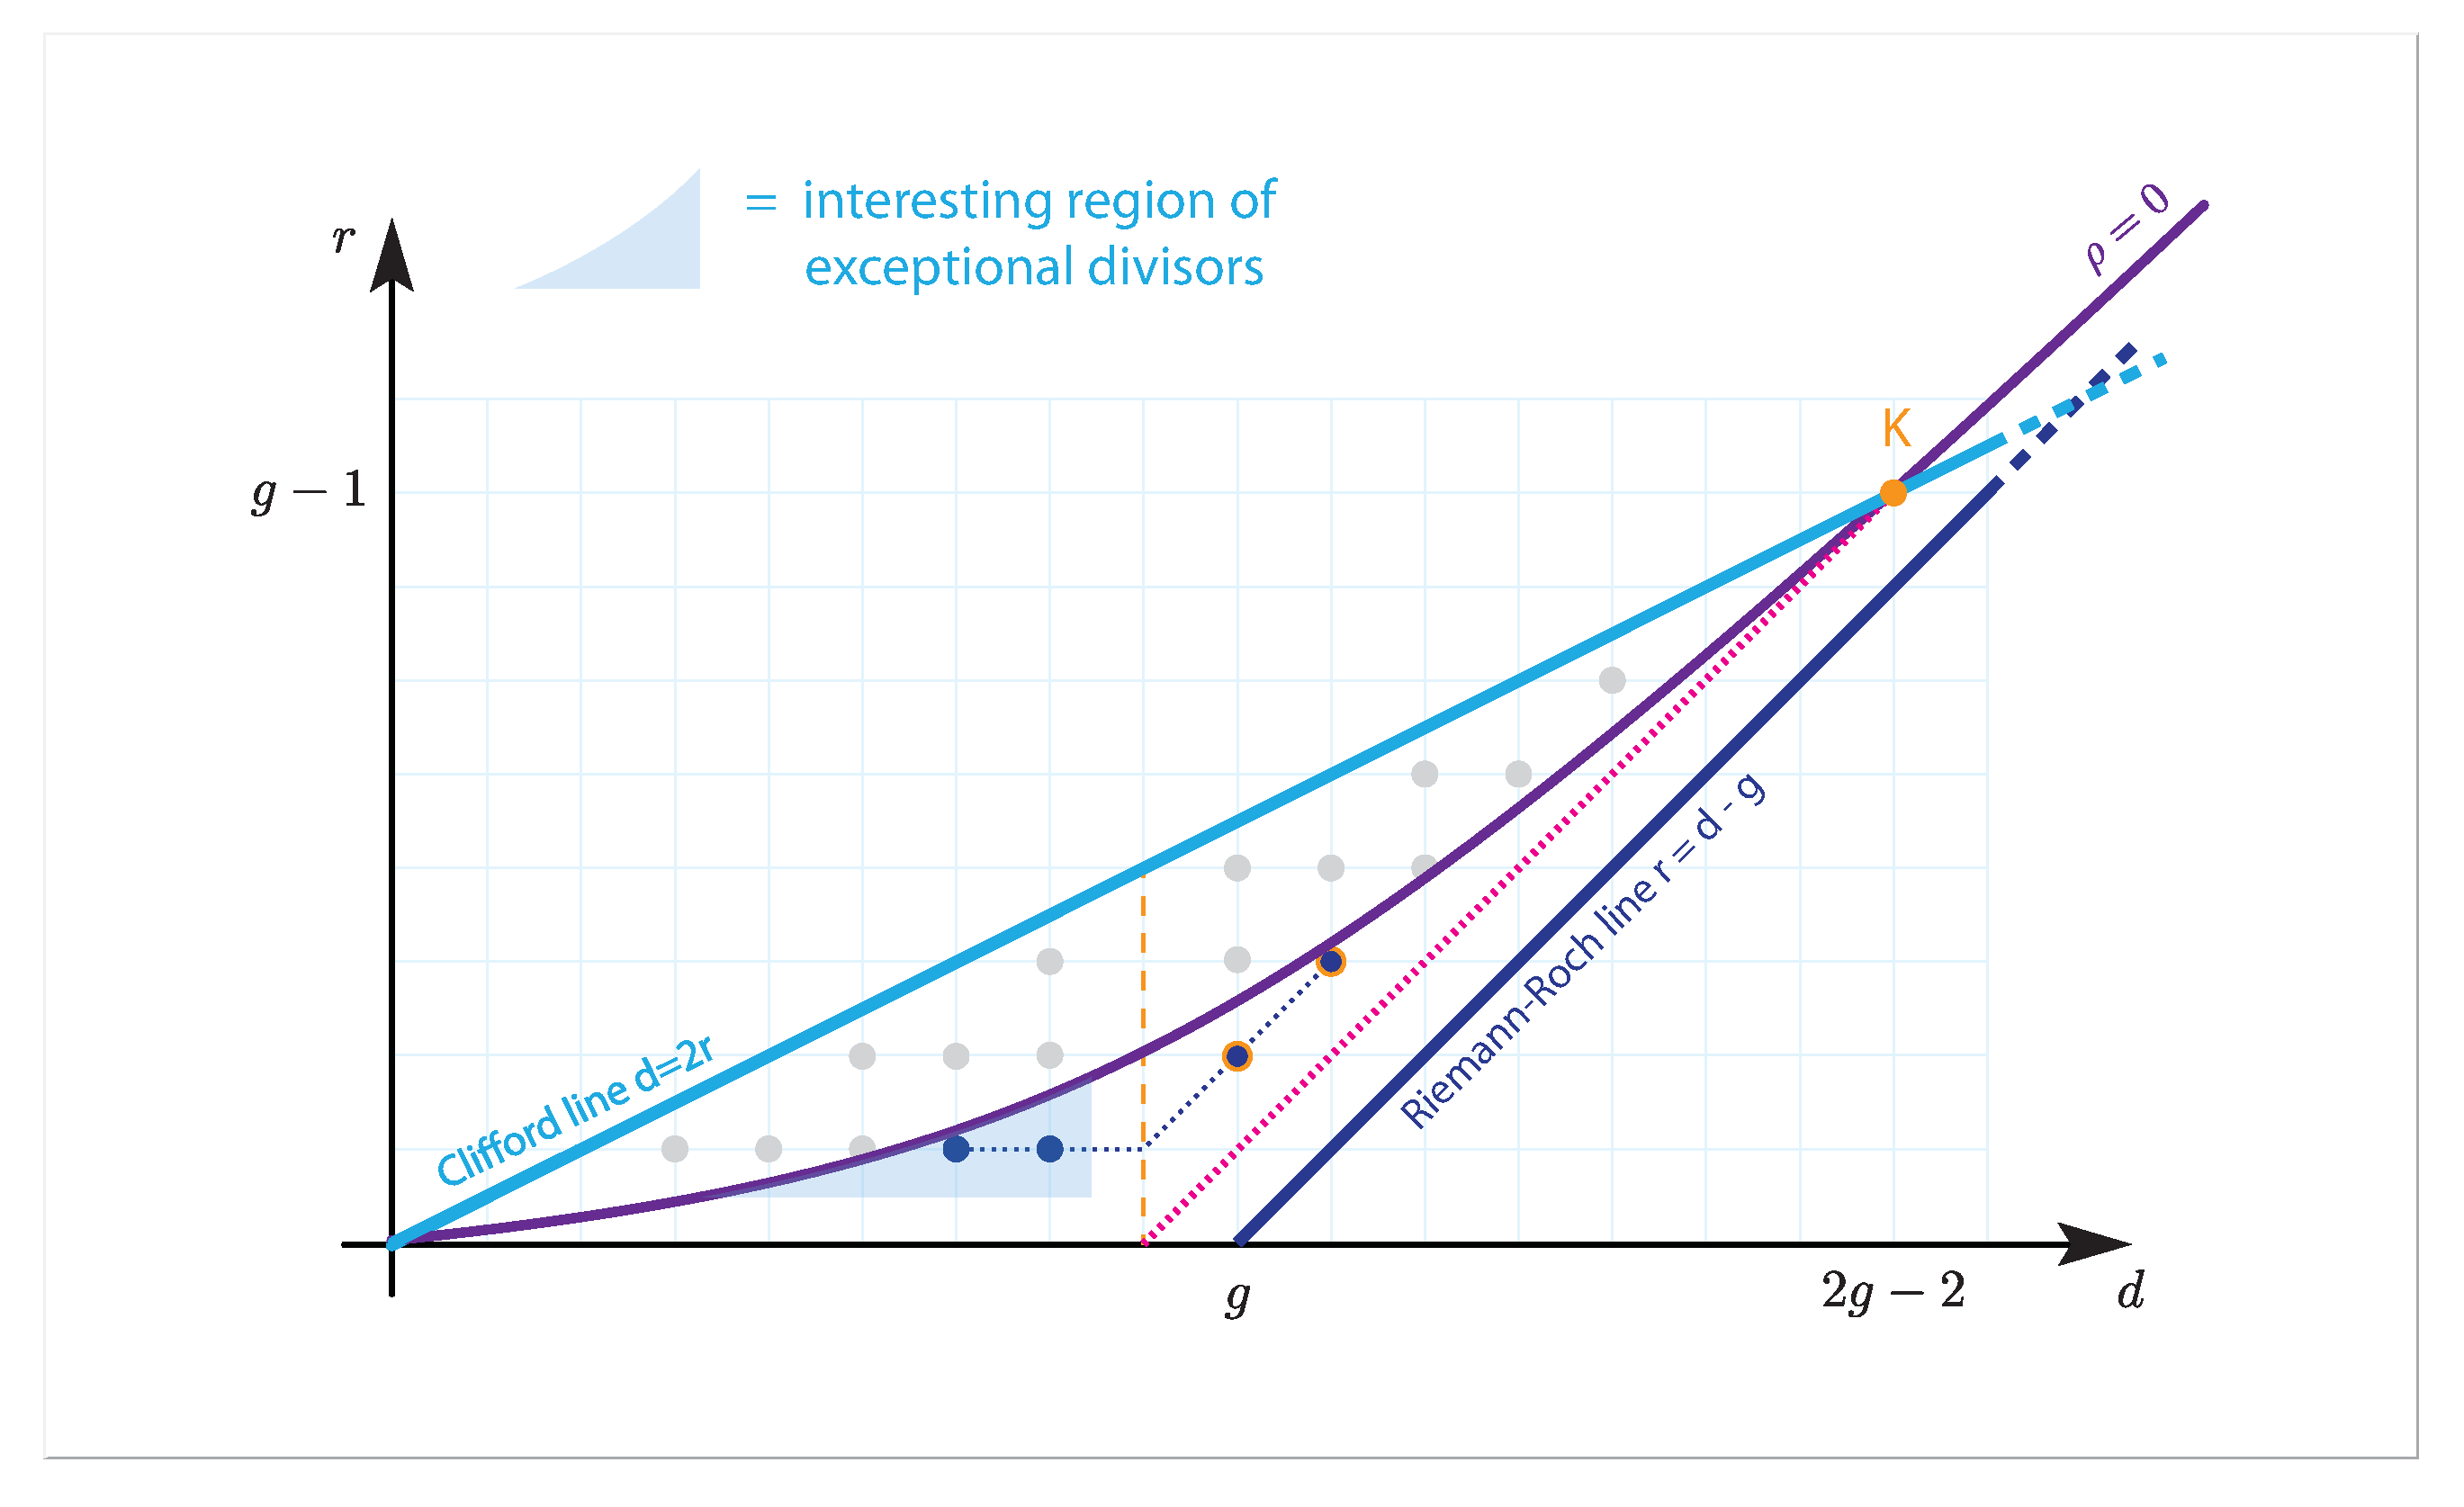
\includegraphics[width=\textwidth]{Exceptional_Divisors_BN.pdf}
		\caption{The interesting region of exceptional special divisors in the case of a curve of genus $g=9$, further refined exploiting the Dimension Theorem }
	\end{figure}









%
% this file is called up by thesis.tex
% content in this file will be fed into the main document

%: ----------------------- name of chapter  -------------------------
\chapter{Appendix A: Some Results in Algebraic Geometry}\label{serre_duality} % top level followed by section, subsection


%: ----------------------- paths to graphics ------------------------

% change according to folder and file names
\ifpdf
    \graphicspath{{figures/}{figures/}{figures/}}
\else
    \graphicspath{{figures/}{figures/}}
\fi

%: ----------------------- contents from here ------------------------

In this Appendix we collect a number of technical results which are exploited in various parts of the Thesis, a solution adopted with the objective of making the main text lighter and more readable.\\ 
For some of the statements a direct proof is given in these pages, while for others we refer to the literature, giving precise references.

\section{Degeneracy loci}
	
	Recall from Section \ref{sec:fitt_deg} the definition of degeneracy ideals $I_n \ph$. A result by Eagon and Northcott on the height of such ideals is exploited in Section \ref{sec:lower_bound} to obtain a lower bound for the dimension of connected components of the varieties \modu.
	\begin{theo}\label{thm:height}
		Let $\ph:E\to F$ be a morphism of locally free sheaves of finite rank $e$ and $f$. Then for every $\mathfrak{p}$ a minimal prime ideal of $I_n \ph$ we have
		$$ \height (\mathfrak{p}) \leq (e-n+1)(f-n+1). $$
	\end{theo}
	\begin{proof}
		See \cite{NORTH}, Theorem 3.
	\end{proof}

	A general result about the degeneracy locus of a vector bundle morphism turns out to be the crucial ingredient we need to get the Existence and Connectedness Theorems. Recall our notation for the $n$-degeneracy locus associated to a morphism $\ph$ of vector bundles over $X$:
	$$ D_{n} (\ph) = \set{ x\in X \mid \rank_x(\ph) \leq n } $$
	\begin{theo}\label{theo:alg}
		Let $Y$ be an irreducible algebraic variety over an algebraically closed field $k$ and $ \ph: E\to F $
		a morphism of vector bundles of dimension $e$ and $f$ over $Y$, such that $ E^*\otimes F$ is ample. Then
			$$ \dim(Y) \geq (e-n)(f-n) \quad\implies\quad D_{n} (\ph) \text{ is not empty } $$
		and
			$$ \dim(Y) > (e-n)(f-n) \quad\implies\quad D_{n} (\ph) \text{ is connected } $$
	\end{theo}
	\begin{proof}
		The Theorem is stated and proved in the case $k=\C$ in \cite{FULTON} (see Theorem 1.1). Moreover, Remark 1.7 of the same article ensures that the result is still valid for an arbitrary algebraically closed field $k$. The argument needs to be modified slightly, using the \'etale cohomology in place of the singular cohomology.
	\end{proof}

\section{Cohomology and base change}
	First of all we recall here a basic result about proper base change and cohomology, appearing for example in the nice book \emph{Abelian Varieties} by David Mumford.
	\begin{namedtheo}[Proper Base Change Theorem]
		Let $f:X\to Y$ be a proper morphism of Noetherian schemes with $Y=\Spec(A)$ affine, and $\scr{F}$ a coherent sheaf on $X$, flat over $Y$. Then there exists a finite complex
		$$ K^\bullet \;:\qquad 0\to K^0\to K^1 \to\dots\to K^n \to 0 $$
		of finitely generated projective $A$-modules, together with a natural isomorphism of functors
		$$ H^p(X\times_Y \square, \scr{F}\otimes_A \square) \cong \mathscr{H}(K^\bullet \otimes_A \square) $$
		on the category of $A$-algebras.
	\end{namedtheo}
	\begin{proof}
		The proof can be found in Chapter $II$, Section $5$ of \cite{MUMAV} -- see the second Theorem.
	\end{proof}	

	As a corollary of the above Theorem we get a statement on the relationship between the direct image and cohomology functors, ensuring that the fibers of $R^\bullet f_*$ coincide with $H^\bullet$ as long as the dimensions of the cohomology groups are fiberwise constant. Since any second cohomology group is trivial on a curve, this result is particularly useful in our context and is exploited more than once.
	\begin{prop}\label{prop:no_jumps}
		Let $f:X\to Y$ be a proper morphism of Noetherian schemes, and $\scr{F}$ a coherent sheaf on $X$, flat over $Y$. Assume $Y$ is reduced and connected, then the following are equivalent for every $i\in \N$
		\begin{enumerate}[(i)]
			\item The function $y\mapsto \dim_{k(y)}H^i(X_y,\, \scr{F}_{\mid y})$ is constant
			\item $R^i f_* \scr{F}$ is a locally free sheaf on $Y$ and the natural map
			$$ R^i f_* \scr{F} \otimes k(y) \to H^i(X_y,\, \scr{F}_{\mid y}) $$
			is an isomorphism for every $y\in Y$.
		\end{enumerate}
		Moreover, if the above conditions are fulfilled, the natural map
		$$ R^{i-1} f_* \scr{F} \otimes k(y) \to H^{i-1}(X_y,\, \scr{F}_{\mid y}) $$
		is an isomorphism for every $y\in Y$.
	\end{prop}
	\begin{proof}
		The proof can be found in Chapter $II$, Section $5$ of \cite{MUMAV} -- see Corollary 2.
	\end{proof}
	Applying the above Proposition to the case of a locally free sheaf $\scr{F}$ with trivial cohomology in positive degrees, we get the following Proposition:
	\begin{prop}\label{prop:R1_trick}
		Let $f:X\to Y$ be a proper morphism of Noetherian schemes with $Y$ reduced and connected, and $\scr{F}$ a coherent sheaf on $X$ with the properties	
		\vspace{0.5em}\\ \vspace{0.5em}	
		\begin{tabular}{ c r }
			\parbox{0.6\textwidth}{\begin{itemize}
				\item $\scr{F}$ is flat over $Y$
				\item $f_*\scr{F}$ is locally free
				\item $R^if_*\scr{F}=0$ for every $i>0$
			\end{itemize} }
			&
			\parbox{0.4\textwidth}{$
				\begin{tikzpicture}[node distance=5em, auto]
					\node (A) 									{$X'$};
					\node (B) 	[right of=A]		{$X$};
				  \node (C) 	[below of=A]	 	{$Y'$};
				  \node (D) 	[below of=B] 		{$Y$};
				  \draw[-stealth][swap]		(A)		to node {$h$} 				(B);
				  \draw[-stealth]					(C)		to node {$g$} 				(D);
				  \draw[-stealth][swap]		(A)		to node {$f'$} 				(C);
				  \draw[-stealth]					(B)		to node {$f$} 				(D);
				\end{tikzpicture}
			$}
		\end{tabular}
		Then for every base change diagram as above, setting $\scr{F}'=h^*\scr{F}$, the natural map $g^* R^i f_* \scr{F} \to R^i f'_*\scr{F}'$ is an isomorphism for every $i\geq 0$.
	\end{prop}
	\begin{proof}
		First observe that on fibres, for every $y\in Y$ and $y'\in Y'$ such that $g(y')=y$, we have isomorphisms
		\begin{equation}\label{eq:fibres}
			H^i(X_y, \scr{F}_{\mid y}) \cong H^i(X_{y'}, \scr{F'}_{\mid y'}) \qquad \forall\; i\geq 0\;.
		\end{equation}
		Next, applying Proposition \ref{prop:no_jumps} and using induction from above, we readily see that our hypothesis of the vanishing of $R^if_*\scr{F}$ in positive degrees implies that
		$$ 
		H^i(X_y, \scr{F}_{\mid y}) = 0 \quad \forall\;i>0 
		\AND 
		H^0(X_y, \scr{F}_{\mid y}) \cong f_* \scr{F}_{\mid y} \;.
		$$ 
		Further, combining the above with \eqref{eq:fibres}, we deduce that the function $y'\mapsto h^i(X_{y'}, \scr{F'}_{\mid y'})$ is constantly equal to zero $\forall\; i>0$, hence -- invoking Proposition \ref{prop:no_jumps} again -- it follows that $R^i f_*' \scr{F}'$ vanishes for positive $i$ and, moreover, that
		$$ H^0(X_{y'}, \scr{F'}_{\mid y'}) \cong f_*'\scr{F}'_{\mid y'} \qquad \forall\; y' \in Y'. $$
		Therefore we deduce -- we can apply Proposition \ref{prop:no_jumps} since $f_*\scr{F}$ is locally free -- that the function
		$$ y'\mapsto h^0(X_{y'}, \scr{F'}_{\mid y'}) = h^0(X_y, \scr{F}_{\mid y}) $$
		is also constant, hence $f_*'\scr{F}'$ is locally free. Since pullbacks preserve locally free sheaves, the sheaf $g^* f_*\scr{F}$ is locally free as well and, as a consequence, we have
		$$ g^* f_* \scr{F}_{\mid y'} = f_* \scr{F}_{\mid y} \cong H^0(X_y, \scr{F}_{\mid y}). $$ 
		Now, for $i>0$ we are done, while for $i=0$ we have a natural map $g^* f_* \scr{F} \to f'_*\scr{F}'$ between two locally-free sheaves. Form the above discussion combined with \eqref{eq:fibres}, it follows that the two sheaves are fiberwise isomorphic and, further, one can check that the isomorphisms on fibres are induced by the natural map, thus getting to the desired conclusion.
	\end{proof}
	\vspace{1em}
	%
	We continue this Section by proving an easy Lemma, which is used more than once during our discussion. The idea is that to kill the higher cohomology of a family of line bundles it is enough to add a divisor of high degree, then the \RR finishes the job.
	\begin{lemm}\label{lemm:trivial_R1}
		Let $X$ be a smooth projective curve over an algebraically closed field, let $T$ be an $S$-scheme and $L$ a family of line bundles of degree $d$ parametrised by $T$. Denote by $\phi:X_T\to T$ the natural projection, pick a divisor $D\subset X$ of degree higher than $2g-d-1$ and let $\Gamma := \phi^* D$ be the product divisor on $X_T$. Then
		$$ R^i\phi_* L = 0 \qquad \forall \;i \geq 1 $$
	\end{lemm}
	\begin{proof}
		Since over any closed point $t \in T$ the line bundle $L_{\mid t}$ has degree $d$, it follows that $L(\Gamma)_{\mid t}$ has degree strictly higher than $2g-2$. Hence from the \RR Theorem we deduce that the function
		$$ t \mapsto \dim H^1(X, L_{\mid t}) $$
		is everywhere vanishing and therefore Proposition \ref{prop:no_jumps} implies that $R^1\phi_* L$ is the trivial sheaf, being locally free with trivial fibres. For $i>1$ a similar argument applies: the only difference is that, since we are working on a curve, we do not even need to invoke the \RRo.
	\end{proof}

	Another well known and useful result is the so called Projection Formula.
	\begin{namedtheo}[Projection Formula]\label{thm:projection_formula}
		Let $f:X\to Y$ be a morphism of locally ringed spaces, $\scr{F}$ an $\OX$-module and $\cal{E}$ a locally free $\OY$-module of finite rank. Then $\forall\, i \geq 0$ we have natural isomorphisms
		\begin{equation}\label{eq:proj_formula}
			R^i f_*( \scr{F}\otimes f^* \scr{E} ) \;\cong\; R^i f_*( \scr{F}) \otimes \scr{E}
		\end{equation}
	\end{namedtheo}
	\begin{proof}
		A proof can be found in \cite[\href{http://stacks.math.columbia.edu/tag/01E8}{Lemma 01E8}]{stacks-project}. Nevertheless, we give here an alternative and more \emph{down-to-earth} proof of the result. \\
		First of all we will show that there is a natural morphism
		$$  f_*\scr{F}\otimes \scr{E} \to f_*(\scr{F}\otimes f^* \scr{E}) $$
		and, to do so, it is useful to recall the following basic results, where we denote by $\HH$ the Hom sheaf prescribed on open sets $U$ as $U\mapsto \Ho(\square_{\mid U}, \square_{\mid U})$
		\begin{enumerate}[(1)]
			\item Adjunction between $\otimes$ and $\HH$
			$$ \Ho_X(\scr{A}\otimes \scr{B},\; \scr{C}) \cong \Ho_X(\scr{A},\; \HH_X(\scr{B},\scr{C})) $$

			\item Adjunction between $f_*$ and $f^*$
			$$\Ho_Y(f_* \scr{F},\; \scr{E} ) \cong \Ho_X (\scr{F},\; f^*\scr{E})$$

			\item Identity which follows from the definitions of $\HH$ and $f_*$
		\end{enumerate}
		$$f_* \mathscr{H}_X(\scr{A},\;\scr{B}) \cong \mathscr{H}_Y(f_* \scr{A},\; f_* \scr{B})$$
		Then, the existence of the above mentioned natural map follows from the chain of isomorphisms: just pick the identity!
		\begin{eqnarray*}
			\Ho_Y(f_*\scr{F}\otimes \scr{E},\; f_*(\scr{F}\otimes f^* \scr{E})) &\overset{(1)}\cong& 
			\Ho_Y(\scr{E},\; \HH_Y(f_*\scr{F},\;f_*(\scr{F}\otimes f^* \scr{E}))) \\
			&\overset{(3)}\cong&
			\Ho_Y(\scr{E},\; f_*\HH_X(\scr{F},\;(\scr{F}\otimes f^* \scr{E}))) \\
			&\overset{(2)}\cong&
			\Ho_X(f^*\scr{E},\; \HH_X(\scr{F},\;(\scr{F}\otimes f^* \scr{E}))) \\
			&\overset{(1)}\cong&
			\Ho_X(\scr{F} \otimes f^*\scr{E},\; \scr{F}\otimes f^* \scr{E})
		\end{eqnarray*}
		We are now going to show that the obtained natural map is in fact an isomorphism. Since all the functors involved commute with open restrictions, we can reduce to the affine case and assume $\scr{E}$ is free. One can check that the above global map agrees with the chain of isomorphisms
		\begin{eqnarray*}
			f_*(\scr{F}\otimes f^*\scr{E}) 
			&\;\cong\;& f_*(\scr{F}\otimes \scr{O}_X^{\,n}) \\
			&\;\cong\;& f_*(\scr{F}\otimes \scr{O}_X)^{n} \\ 
			&\;\cong\;& f_*(\scr{F})^{n} \\
			&\;\cong\;& f_*(\scr{F})\otimes \scr{O}_Y^{\,n} \\
			&\;\cong\;& f_*(\scr{F})\otimes \scr{E}
		\end{eqnarray*}
		where we used multiple times the fact that the functors involved are additive and thus commute with finite direct sums. The obtained isomorphism implies that
			$$ R^i f_*(\scr{F}\otimes f^*\scr{E}) \;\cong\; R^i (f_*(\scr{F})\otimes \scr{E}) \;\cong\; R^i f_* (\scr{F}) \otimes \scr{E} $$
			 for every $i\in \N$. For the second isomorphism we used the well known fact that \emph{tensoring with a locally free module} is an exact functor.
	\end{proof}

\section{Line Bundles}
	In Section \ref{sec:ampleness} we need to show that a certain line bundle of interest is ample and, to do so, we exploit the combination of the following criterions for ampleness together with the next Lemma.
	\begin{prop}\label{prop:Nakai}
		Let $f:X\to Y$ be a finite and surjective morphism between proper Noetherian schemes and $L$ a line bundle over $Y$. Then $L$ is ample \ABiff its pullback $f^*L$ is.
	\end{prop}
	\begin{proof}
		We refer to \cite{HAG}, where the result is given in Ex. III.5.7.d.
	\end{proof}

	\begin{prop}\label{prop:Nakai_Moishezon}
		Let $Y$ be a smooth projective surface. Then the line bundle corresponding to a Cartier divisor $D$ is ample \ABiff the self-intersection number $D^2$ is strictly positive and $C\cdot D >0$ for every irreducible curve $C\subset Y$. 
	\end{prop}
	\begin{proof}
		We refer to \cite{HAG}, Theorem V.1.10.
	\end{proof}


	\begin{lemm}\label{lemm:tensor_ampleness}
		For every $i=1,\dots n$, let $Y_i$ be a smooth projective curve over an algebraically closed field $k$ and $M_i$ an ample line bundle on $Y_i$. Further let $Y=Y_1\times\dots\times Y_n$ and denote by $\pi_i:Y \to Y_i$ the projection on the $i$-th component. Then the line bundle
		$ \otimes_{i=1}^n \pi_i^* M_i $
		over $Y$ is ample.
	\end{lemm}
	\begin{proof}
		We will prove the claim for the case $n=2$, then the general result easily follows by induction over $n$. Notice that $Y_1 \times Y_2$ is a smooth projective surface. \\

		Set $L=\pi_1^*M_1 \otimes \pi_2^*M_2$. Since $M_1$ and $M_2$ are ample, replacing $L$ with $L^{\otimes m}$ with $m$ big enough ( if needed ) we see that $L$ admits a section which corresponds to the effective divisor
		$$ D = \sum_a F_a + \sum_b G_b $$
		where each $F_a$ is a fiber of $\pi_1$ and each $G_b$ is a fiber of $\pi_2$. Notice that, since the surface $Y_1 \times Y_2$ is the product of two curves, all such fibres are algebraically equivalent. Hence, given an irreducible curve $C\subset Y$, we can choose the fibres $F_a$ and $F_b$ in such a way that the intersection between $C$ and $D$ is proper, so that we get $C\cdot D > 0$. Moreover, this argument applies to the case $C=D$ as well, therefore also $D^2>0$ and by Proposition \ref{prop:Nakai_Moishezon} we conclude that $L$ is ample.
	\end{proof}	


	\begin{comment}
		\begin{lemm}\label{lemm:tensor_ampleness}
			Let $X$ be a proper Noetherian variety and $L_1, \dots, L_m$ a finite number of ample line bundles over $X$. Then their tensor product $ \otimes_{i=1}^m L_i $ is ample.
		\end{lemm}
		\begin{proof}
			We will prove the claim for a pair of line bundles $L$ and $M$, then the general result easily follows by induction over $m$.\\

			Since $X$ is proper and Noetherian the Cartan-Serre-Grothendieck Theorem holds and, thus, an equivalent condition for the ampleness of $L$ is the existence of a natural number $m\in \N$ such that for every coherent sheaf $\scr{F}$ on $X$ we have
			$$ H^i(X, \scr{F}\otimes L^{\otimes n}) = 0 \qquad \forall \; i\geq 1 \,. $$
		 	Now let $\scr{E}$ be any coherent sheaf on $X$ and notice that, in particular, the above condition holds for the coherent $\scr{F} = \scr{E}\otimes M^{\otimes n}$. Therefore for every $i\geq 1$ we find
		 	$$ H^i(X, \scr{E}\otimes (L\otimes M)^{\otimes n} ) = H^i(X, \scr{F}\otimes L^{\otimes n} ) = 0 $$
		 	and, hence, by another application of the Cartan-Serre-Grothendieck Theorem we see that $L\otimes M$ is ample.
		\end{proof}	
	\end{comment}	

	We now prove a Lemma about the behaviour of line bundles over a product with a complete factor, which we use in Section \ref{sec:defi_modu}.
	\begin{lemm}\label{lemm:square}
		Let $X$ and $Y$ be schemes, with $X$ complete and $L,M$ line bundles over $X\times Y$ such that $\forall y\in Y$ we have $L_y \cong M_y$. Then there exists a line bundle $F$ over $Y$ such that $L\cong M\otimes \pi^* F$, where $\pi :X \times Y\to Y$ is the natural projection.
	\end{lemm}
	\begin{proof}
		Let $F=L\otimes M^{-1}$ and notice that, since $F_y$ is trivial and $X$ is complete, for every $y\in Y$ we have $H^0(X, F_y)=k(y)$. Hence the function
		$$ y \mapsto \dim_{k(y)} H^0(X, F_y) $$
		is constantly equal to $1$. Therefore, by Proposition \ref{prop:no_jumps}, $\pi_* F$ is locally free of rank $1$, i.e.\ it is a line bundle over $Y$. Now, if we show that the natural map 
		$$ \ph: \pi^*\pi_* F \to F $$
		is an isomorphism, we are done. On every fiber the above map restricts to the isomorphism
		$$ \OX \otimes H^0(X, \OX) \toiso \OX $$
		so by Nakayama's lemma we deduce that $\ph$ is surjective. But rank is invariant under pullback, so $\pi^* \pi_* F$ has rank $1$, thus forcing $\ph$ to be an isomorphism.
	\end{proof}

	Finally, we prove that line bundles on $X_T/T$ with the canonical rigidification discussed in Section \ref{sec:Pic_functor} admit no nontrivial automorphisms. This is the main reason why one defines the relative Picard functor as in Section \ref{sec:Pic_functor}, since the absence of automorphisms allows for its representability.
	\begin{prop}\label{prop:rigid}
		Under hypothesis and notation of $(\star)$ from Section \ref{sec:assumptions}, line bundles on $X_T/T$ with the canonical rigidification along $\eps_T$ have no nontrivial automorphisms. 
	\end{prop}
	\begin{proof}
		First of all, to make the setting clear, let us draw the fibered diagram we are working with, filled with the sections we have at our disposal (we  abuse notation and write $\eps$ also for the pullback morphism $\eps_T$). Further, we draw the diagram describing a morphism of line bundles with rigidification on the right.
		
		\begin{equation*}
		\begin{tikzpicture}[node distance=5em, auto] %SQUARE
			\node (A) 															{$X_T$};
			\node (B) 	[right of=A, xshift=3em]		{$T$};
		  \node (C) 	[below of=A] 								{$X$};
		  \node (D) 	[right of=C, xshift=3em] 		{$S$};
		  %
		 	\node (A2) 	[right of=B, xshift=3em]			{$\calO_T$};
			\node (B2) 	[right of=A2, xshift=2em]			{$\eps^*L_1$};
		  \node (C2) 	[below of=A2] 								{$\calO_T$};
		  \node (D2) 	[right of=C2, xshift=2em] 		{$\eps^*L_2$};
		  %
		  \draw[-stealth, bend left=15, looseness=1]						(A)		to node {$f$} 			(B);
		  \draw[-stealth, bend left=15, looseness=1]						(B)		to node {$\eps$} 	(A);
		  \draw[-stealth]																				(A)		to node {} (C);
		  \draw[-stealth]																				(B)		to node {} (D);
		  \draw[-stealth, bend right=15, looseness=1, swap]			(D)		to node {$\eps$}		(C);
		  \draw[-stealth, bend right=15, looseness=1, swap]			(C)		to node {$f$} 			(D);
		  %
		  \draw[-stealth]						(A2)		to node {$\al_1$} 				(B2);
		  \draw[-stealth, swap]			(A2)		to node {$=$} 						(C2);
		  \draw[-stealth]						(B2)		to node {$\eps^*\ph$} 	(D2);
		  \draw[-stealth, swap]			(C2)		to node {$\al_2$}					(D2);
		\end{tikzpicture}
		\end{equation*}
		
		Recall that a morphism between two line bundle with rigidification $\ph:(L_1,\al_1) \to (L_2,\al_2)$ consists of a morphism of (plain) line bundles $\ph:L_1\to L_2$ such that $(\eps^* \,\ph)\,\al_1 = \al_2$ and, in particular, an endomorphism is an element $h\in \Gamma(X_T, \calO_{X_T})$ such that $\eps^* \,h = 1$. But from of our assumption $f_*\calO_{X_T} \cong \calO_T$, contained in $(\star)$, we get isomorphisms
		$$ \Gamma(X_T, \calO_{X_T}) \cong \Gamma(T, f_*\calO_{X_T}) \underset{(\star)}\cong \Gamma(T, \calO_{T}) $$
		and we therefore see that the only automorphisms are the trivial ones.
	\end{proof}

\section{Tangent space of schemes}
	The following basic lemmata allow us to compute the tangent spaces of the schemes $\EDiv_X$ and $\Pic_X$ in Section \ref{sec:tgnt_spaces}. Recall that we use the notation $k_\eps$ for the ring of dual numbers $k[\eps]/\eps^2$.
		\begin{lemm}\label{lemm:tng_sch}
		Let $P$ be a scheme over $S=\Spec(k)$ locally of finite type and $e\in P$ a rational point. Then we have an isomorphism of vector spaces
		$$ P(k_\eps)_e \; \cong \; T_e P. $$
	\end{lemm}
	\begin{proof}
		Let $\frakm$ be the maximal ideal of $e$ and $A$ its local ring. The Zariski tangent space at $e$ is $\Hom(\frakm/\frakm^2, k)$, which can naturally be identified with the set of $k$-derivations $\delta:A\to k$. To any such derivation corresponds bijectively a $k$-map
		$$ u_\delta : A \to k_\eps, \quad a\mapsto a \text{ mod } \frakm + \eps\delta(a), $$
		as it is easy to show. Further, any such map gives rise to a unique map of schemes
		$$ t_\delta : \Spec(k_\eps) \to P $$
		which is supported at $e$, and viceversa. Therefore we proved that $P(k_\eps)_e \cong T_e P$ as sets. We now want to see how the vector space structure of $T_e P$ transfers to $P(k_\eps)_e$, starting from the multiplication by scalars. For $b\in k$ it is easy to check that the $k$-map
		$$ \mu_b : k_\eps\to k_\eps, \quad \eps \mapsto b\cdot \eps $$
		corresponds to multiplication by $b$ in $T_eP$. Therefore scalar multiplication by $b$ on $P(k_\eps)_e$ is given by the map
		$$ P(\mu_b) : P(k_\eps)_e \to P(k_\eps)_e. $$
		For the additive structure, first define $k_{\eps,\eps'}$ to be the ring obtained by adjoining to $k_\eps$ an element $\eps'$ such that $\eps'^2 = \eps\eps' = 0$. Secondly define maps $\sigma_1,\sigma_2 : k_{\eps,\eps'}\to k_\eps$ by
		$$ \sigma_1: \eps\mapsto \eps,\; \eps'\mapsto 0, \qquad \sigma_2: \eps\mapsto 0,\; \eps'\mapsto \eps $$
		and use them to get a bijection $\pi:P(k_{\eps, \eps'})_e \toiso P(k_\eps)_e \times P(k_\eps)_e $. Further, let
		$$ \sigma: k_{\eps,\eps'}\to k_\eps, \qquad \eps\mapsto \eps,\; \eps'\mapsto \eps $$
		and finally set $\al = P(\sigma)\circ \pi^{-1}$. It is now a triviality to check that $\al$ corresponds to summation in $T_eP$.
	\end{proof}
	\begin{comment}
		It would be nice to give here a geometrical interpretation of the above result, together with a picture.
	\end{comment}
	In the case of a group scheme we can state a slightly more powerful result:
	\begin{lemm}\label{lemm:tng_grp_sch}
		Let $P$ be a group scheme over $S=\Spec(k)$ locally of finite type and $e\in P$ the identity element. Then we have an isomorphism of vector spaces
		$$ T_e P \;\cong\; \ker \Big( P(k_\eps) \to P(k) \Big). $$
	\end{lemm}
	\begin{proof}
		The natural map of rings $k_\eps \to k$ gives rise to a map of schemes $\rho: P(k_\eps) \to P(k)$ whose kernel is $P(k_\eps)_e \cong T_e P$. So to conclude we just need to show that the sum on $T_eP$ corresponds to the group operation of $\ker(\rho)$, i.e., using the notation of the previous lemma, that we have
		$$ \al(m,n)= m \cdot n. $$
		Let $i:k_\eps \to k_{\eps,\eps'}$ be the natural inclusion and notice that the map $\sigma_2 \circ i$ factors via $k_\eps\to k$. Thus for every $m\in P(k_\eps)_e$ we find $P(\sigma_2)\circ P(i)(m)=e$. Moreover the maps $\sigma\circ i$ and $\sigma_1\circ i$ coincide with the identity of $k_\eps$, which implies
		$$ P(\sigma)\circ P(i)(m)=m \AND \pi\circ P(i)(m) = (m,e). $$
		Hence we deduce
		$$ \al(m,e) = P(\sigma)\circ \pi^{-1}(m,e) = P(\sigma)\circ P(i)(m) = m $$
		and similarly $\al(e,n) = n$. Since $\al$ arises from the composition of two ring homomorphisms, it is a group homomorphism and therefore
		$$ \al(m,n) = \al(m,e)\cdot\al(e,n) = m\cdot n $$
		as desired.
	\end{proof}

\section{Clifford's Theorem}

	This Section is dedicated to the famous Theorem of Clifford, which gives an upper bound on the dimension of linear series. In order to prove it, we first need some preliminary results.
		\begin{lemm}
		For a divisor $D$ on a curve $X$ we have $\dim|D|\geq k$ \ABiff for every set of $k$ points $p_1, \dots, p_k$ of $X$ there exists an element of $|D|$ containing all of them.
	\end{lemm}
	\begin{proof}
		If for every set of $k$ points $p_1, \dots, p_k$ of $X$ there exists a divisor in $|D|$ containing all of them, then trivially $\dim|D|\geq k$ since the family $\sum_{i=1}^d p_i$ is $k$-dimensional.\\
		Conversely, assume $\dim|D|\geq k$ and pick $k$ points $p_1, \dots, p_k$ of $X$. We have 
		$$ h^0(X, D - \sum_{i=1}^d p_i) \geq h^0(X, D) - k \geq 1, $$
		so that there exists a global section $f\in H^0(X, D - \sum_{i=1}^d p_i)$ such that 
		$$ (f)+D-\sum_{i=1}^d p_i \geq 0 \iff D' = (f)+D \geq \sum_{i=1}^d p_i, $$
		therefore $D'$ is an element of $|D|$ containing all the points.
	\end{proof}
	\begin{coro}
		Let $D_1$ and $D_2$ be two effective divisors of $X$. Then
		$$ \dim|D_1| + \dim|D_2| \leq |D_1+D_2|. $$
	\end{coro}
	\begin{proof}
		Assume $d_i=\dim(D_i)$ and let $p_1,\dots,p_{d_1}$ and $q_1,\dots,q_{d_2}$ be points of $X$. Then by the lemma we can find divisors $D_1'\in |D_1|$ and $D_2'\in |D_2|$ containing respectively $p_1,\dots,p_{d_1}$ and $q_1,\dots,q_{d_2}$. Therefore the divisor $D_1'+D_2' \in |D_1+D_2|$ contains all of the $d_1+d_2$ points and, applying the lemma again, we find
		$$ \dim|D_1 + D_2| \geq d_1 + d_1. $$
	\end{proof}
	We now state another useful Lemma, for which we need the following well-known fact about the non-degeneracy of the canonical image
	\begin{prop}
		Let $d\leq g$, and $X$ a curve of genus $g$. Then any $d$ points of the canonical image $\phi(X)$ are linearly independent, i.e. they span a $\PP^{d-1}.$
	\end{prop}
	\begin{lemm}\label{lemm:hyp_linear}
		Let $X$ be a hyperelliptic curve of genus $g$, and $d\leq g$. Then any complete $g_d^r$ on $X$ is of the form
		$$ r\cdot g_2^1 + P_1 + \dots + P_{d-2r}, $$
		where none of the $P_i$ is conjugate under the hyperelliptic involution.
	\end{lemm}
	\begin{proof}
		Almost immediate using the above proposition.
	\end{proof}
	Now we are almost ready to prove the crucial Clifford's theorem, which gives a bound to the dimension of the complete linear system $|D|$. But first we need another classical result, i.e.\ the
	\begin{namedtheo}[General Position Theorem]\label{thm:GPT}
		Let $r\geq 2$ and $X\subset \PP^r$ be an irreducible nondegenerate curve of degree $d$. Then a general hyperplane cuts $X$ in $d$	points, any $r$ of which are linearly independent.
	\end{namedtheo}
	A proof of the above theorem can be found in \cite{GAC}. Next, we finally move to the
	\begin{namedtheo}[Clifford's Theorem]\label{thm:Clifford}
		Let $D$ be an effective divisor on a curve $X$ with $d = \deg(D) \leq 2g-2$. Then we have:
		\begin{enumerate}[(i)]
			\item $ \dim|D| \leq \frac{d}{2}. $
			\item The equality holds only if $D=0$, $D=K$ or, in case $X$ is hyperelliptic, if $D$ is a multiple of the hyperelliptic involution.
		\end{enumerate}
	\end{namedtheo}
	\begin{proof}
		Before beginning with the proof, recall that a divisor $D$ is called \textbf{special} if $h^0(K-D) > 0$.
		\begin{enumerate}[(i)]
			\item If $D$ is not special then by the \RR we get
			$$ h^0(D) = d-g+1 \iff \dim|D| = d-g $$
			which by hypothesis is strictly lower than $d/2$, since $g \geq d/2+1 $. If $D$ is special, instead, there exists an effective divisor $D'$ such that $K=D+D'$. Therefore applying the above corollary we find
			$$ \dim|D| + \dim|D'| \leq \dim|K| = g-1.  $$
			Moreover, since $D' = K-D$, the Riemann-Roch formula gives
			$$ \dim|D| - \dim|D'| = d - g + 1. $$
			Adding up the two equations we obtain the result.
			
			\item If the equality holds we have
			$$ r(D) + r(D') = g-1.  $$
			Since the degree of $K=D+D'$ is $2g-2$, without losing generality we can assume $\deg(D)\leq g-1$ and from part (i) it follows that 
			$$ r(D)=0 \implica \deg(D')=2g-2 \implica D\sim 0. $$ 
			Otherwise, let $r(D)>0$ and suppose $X$ is not hyperelliptic. From the geometric \RR we know that any hyperplane of $\PG$ cuts $X$ in $\deg(D)\leq g-1$ points of $E\in|D|$ which are not independent (recall that $r(D)>0$ means there is at least one linear relation among them). But this contradicts the general position theorem, therefore $r(D)>0$ forces $X$ to be hyperelliptic. In this case using Lemma $\ref{lemm:hyp_linear}$ we know that any complete $g_d^r$ on $X$ is of the form
			$$ |D| = r\cdot g_2^1 + P_1 + \dots + P_{d-2r} $$
			and, since we are assuming $d=2r$, we see that $|D|$ is a multiple of the hyperelliptic involution.
		\end{enumerate}
	\end{proof}

 %Appendix A - Algebraic Results
% this file is called up by thesis.tex
% content in this file will be fed into the main document

%: ----------------------- name of chapter  -------------------------
\chapter{Appendix B: Serre Duality and Riemann-Roch}\label{serre_duality} % top level followed by section, subsection


%: ----------------------- paths to graphics ------------------------

% change according to folder and file names
\ifpdf
    \graphicspath{{figures/}{figures/}{figures/}}
\else
    \graphicspath{{figures/}{figures/}}
\fi

%: ----------------------- contents from here ------------------------

In this Chapter we give the statement and a proof of the \RR Theorem. As we will see, the \emph{cheap} version of the result can be easily obtained, while the complete statement heavily relies on the Serre Duality Theorem, which we prove in Section \ref{sec:Serre_duality} following the original work of Serre.\\ 
Further, in Section \ref{sec:alpha_delta} we give a motivation for the fact that the restriction map 
$$ \al:H^0(K)\to H^0(K\otimes \OD) $$ 
is, with respect to the Serre duality pairing, dual to the cohomological coboundary map 
$$\delta:H^0(D)_D\to H^1(\OX).$$

\section{Cheap Riemann-Roch}
	In this section we state and prove the \emph{cheap version} of the fundamental \RR theorem. We will be able to prove the complete version of the theorem at the end of this Appendix, exploiting Serre duality.
	\begin{namedtheo}[Cheap \RR Theorem]\label{thm:cheap_RR}
		Let $X$ be a complete curve of genus $g$, $K$ a canonical divisor and $D\in \Dd$. Then
		$$ h^0(D) - h^1(D) = \deg(D)-g+1. $$
	\end{namedtheo}
	\begin{rema}
		The \textbf{Euler characteristic} of a line bundle $L$ over a curve $X$ is defined as
		$$ \chi(L) = h^0(X,L) - h^1(X,L), $$
		so we can rewrite the statement of the \RR as
		$$ \chi(D) = \deg(D) - g + 1. $$
	\end{rema}
	\begin{proof}
		We first prove the theorem for effective divisors $D\geq 0$, proceeding by induction over $d=\deg(D)$. For $d=0$ we obtain $\OD=\OX$ and, since by definition $g=h^1(\OX)$, the formula holds trivially
		$$ h^0(\OX) - h^1(\OX) = 1-g. $$
		Now suppose the relation holds for all effective divisors with $\deg<d$. Let $D'\geq 0$ be of degree $d-1$ and set $D=D'+P$ for $P\in X$. We have a short exact sequence of quasi-coherent sheaves
		$$ \SES{\calO(D')}{\OD}{k_P}, $$
		where $k_P$ is the skyscraper sheaf at $P$ and the map ${\OD}\to{k_P}$ is the evaluation at $P$. Thus using the fact that the Euler characteristic is additive on \sess we obtain
		$$ \chi(D) = \chi(D') + 1 = (d-1-g+1) + 1 = d-g+1, $$
		as required. For the general case $D=D_1-D_2$ with $D_i$ effective of degree $d_i$ we have the \ses
		$$ \SES{\OD}{\calO(D_1)}{k^{d_2}} $$
		which easily leads to the desired result.
	\end{proof}

\section{Serre Duality Theorem}\label{sec:Serre_duality}

	This Section is based on the first chapter of the wonderful book \emph{Algebraic Groups and Class Fields} written by Serre, which appears as entry number \cite{SERRE} in our Bibliography.\\

	Even though Serre duality for curves can be derived as a consequence of Grothendieck's duality Theorem (see for instance Theorem III.7.6 of \cite{HAG}), we will give a more direct proof for the case of curves, inspired by the classical proof used by Weil. A crucial ingredient is the the ring of repartitions, which we now introduce.
	\begin{defi}
		Define $R$, the \textbf{ring of repartitions} on $X$, as the set of collections $\{r_P\}_{P\in X}$ such that $r_P\in k(X)$ for every $P\in X$ and $r_P\in \calO_{X,P}$ for all but finitely many $P\in X$. This is a very big ring, containing in particular $k(X)$, but can also be seen as a $k$-vector space.
		Further, for any divisor $D\in \Div_X$, we define $R(D)$ to be the $k$-vector subspace of $R$ consisting of those repartitions $r$ for which
		$$ v_P(r_P) + v_P(D) \geq 0, \qquad \forall P\in X. $$
	\end{defi}
	As one can easily guess, the space $R(D)$ is strictly related to the invertible sheaf $\OXD$. The following proposition will make this idea precise, but first we need an easy Lemma.
	\begin{lemm}\label{lemm:H1}
		Let $X$ be an irreducible topological space and $\uA$ a constant sheaf of abelian groups on $X$. Then
		$$ H^1(X, \uA) = 0 $$
	\end{lemm}
	\begin{proof}
		Let $\{ U_\al \}_{\al \in I}$ be an open cover of $X$ and $(g_{\alb})$ be a $1$-cocycle in $Z^1(X, \uA)$. Since $X$ is irreducible, the constant presheaf $\uA^{\presheaf}$ is already a sheaf, thus we can fix $i\in I$ and define the $0$-cochain
		$$ h_\al := g_{\al, i} \qquad \forall \al \in I. $$
		The coboundary condition on $(g_{\alb})$ implies that
		$$ \partial (h_\al) = (h_\al - h_\beta) = (g_{\al, i} + g_{i, \beta}) = (g_{\alb}) $$
		so we see that $(g_{\alb})$ is a coboundary and it is therefore trivial in $H^1(X, \uA)$.
	\end{proof}
	\begin{rema}
		A shorter proof of the above Lemma can be given in terms of Grothendieck's functorial definition of sheaf cohomology. The point is that constant sheaves on algebraic varieties are \textbf{flasque}, and these have trivial cohomology in positive degrees. See Proposition $2.5$, Chapter III.2 of \cite{HAG}.
	\end{rema}
	\begin{prop}\label{prop:h1D}
		There is a canonical isomorphism $ H^1(D) \cong \frac{R}{R(D)+k(X)} $.
	\end{prop}
	\begin{proof}
		Let $\underline{k(X)}$ denote the constant sheaf with stalks $k(X)$ and let $S$ be the cokernel of the natural inclusion $\OXD\into \underline{k(X)}$. We thus have a \ses of invertible sheaves
		$$ \SES{\OXD}{\underline{k(X)}}{S} $$
		which, since by Lemma \ref{lemm:H1} we know $H^1(\underline{k(X)})=0$, gives the following exact sequence in cohomology
		$$ 0\to H^0(D)\to k(X) \to H^0(S) \to H^1(D) \to 0. $$
		Hence we just need to show that $H^0(S) \cong R/R(D)$ to be done. In order to do so recall that, by definition of quotient sheaf, $S$ is the sheaf corresponding to the pre-sheaf $S^{\presheaf}$ with stalks at $P$ given by
		$$ S_P := \frac{k(X)}{\OXD_P} $$
		Notice, moreover, that $R/R(D)$ is the direct sum of $S_P$ over all points of $X$
		$$ R/R(D) = \bigoplus_{P\in X} S_P $$
		so it suffices to show that $H^0(S)=\bigoplus_{P\in X} S_P$ get the conclusion. To see it, pick an arbitrary $P\in X$ and consider a nonzero element of the the stalk $S_P$. Extend it to a section $s\in \Gamma(U,S)$ locally defined in a neighborhood $U$ of $P$ and observe this implies that $s$ has a pole at $P$ -- otherwise it would be zero in the stalk $S_P$. Since the locus of points where $s$ is singular is a Zariski closed subset of $X$, we can find a smaller open $U'\subset U$ containing no other singularities of $s$ apart from $P$. Hence we have $s\equiv 0$ on $U'\setminus P$, so it follows that $S^{\presheaf} = S$ is a sheaf on its own right and moreover, since $X$ is complete and any discrete compact set is finite, we see that $S$ is a direct sum of skyscraper sheaves: $S=\bigoplus_{P\in X} (i_P)_* S_P$, where $i_P:P\into X$ is the inclusion of $P$ in $X$. Therefore we find
		$$ H^0(S) = H^0\left(\bigoplus_{P\in X} (i_P)_* S_P \right) = \bigoplus_{P\in X}S_P $$
		as desired.
	\end{proof}
	\begin{defi}
		Given a divisor $D$, define $J(D) := H^1(D)^{\vee}$. 
	\end{defi}
	From the above proposition it follows that $J(D)$ is the space of linear functionals $H^1(D)\to k$ which vanish on $R(D)$ and $k(X)$. Hence it follows that $J(D)\subset J(D')$ \ABiff $D'\leq D$, and we can consider the direct system
	$$ \set{ J(D) \mid D\in \Div_X } $$
	over the directed set $\set{ \Div_X, \preceq }$, where we set $D\preceq D' \iff D' \leq D$. Then we define $J$ to be direct limit of the $J(D)$'s with respect to the above direct system which, since we are taking the limit simply over the inclusion maps, coincides with the union over all divisors $D\in \Div_X$ of the sets $J(D)$.
	\begin{rema}
		Notice that $J$ has a natural structure of vector space over $k(X)$: if $\al\in J(D)$ and $f\in H^0(E)$ then the product $f\cdot\al$ belongs to $J(D-E)\subset J$.
	\end{rema}
	We can give a very strict bound on the dimension of $J$ which will be essential to prove Serre duality. 
	\begin{prop}\label{prop:dim1}
		The dimension of $J$ as a vector space over $k(X)$ is at most $1$.
	\end{prop}
	\begin{proof}
		Suppose $\al$ and $\beta$ are two elements of $J$ which are linearly independent over $k(X)$ and notice that we can always find a divisor $D$ of degree $d$ such that $\al,\beta \in J(D)$. Further, observe that for any divisor $E$ of degree $e$ and functions $f,g \in H^0(E)$ we have
		$$ f \al \in J(D-E) \AND  g\beta \in J(D-E). $$
		The assumption that $\al$ and $\beta$ are linearly independent implies that the map
		$$ \ph: H^0(E)\times H^0(E) \to J(D-E) \qquad (f,g) \mapsto f\al + g\beta $$
		in an injection, therefore looking at the dimensions of the source and the target we deduce that
		$$ h^1(D-E) \geq 2 h^0(E) $$
		and using Theorem \ref{thm:cheap_RR} (Cheap Riemann Roch) we can rewrite the above inequality as
		$$ h^0(D-E)-(d-e) + g - 1 \geq 2(h^1(E)+e-g+1) \geq 2(e-g+1). $$
		In order to get the desired contradiction is now sufficient to notice that for any choice of $e=\deg(E) > d$ we have $h^0(D-E)=0$ and thus we get
		$$ 3g-3-d \geq e, $$
		clearly absurd due to the arbitrary of $e$.
	\end{proof}
	It is now finally the time to define the pairing that will give us Serre duality.
	\begin{defi}
		Let $A$ denote the space of Abelian differentials on $X$, and define the map
		$$ \pairing : R \times A \to k , \qquad \pair{r}{\omega} := \sum_{P\in X} \Res_P(r_P \cdot \omega) $$
		where we take as the definition of residue the one given in Chapter $7$ of \cite{SERRE}, which is purely algebraic.
	\end{defi}
	\begin{lemm}\label{lemm:pairing_properties}
		The map $\pairing$ has the following properties:
	\begin{enumerate}[(i)]
		\item $ r\in R(D),\; \w \in H^0(K-D) \implies \pair{r}{\w} = 0 $
		\item $ r\in k(X) \implies \pair{r}{\w}=0 $
		\item $ f\in k(X) \implies \pair{fr}{\w} = \pair{r}{f\w} $
	\end{enumerate}
	\end{lemm}
	\begin{proof}\mbox{}\\*
		\begin{enumerate}[(i)]
			\item Any repartition $r\in R(D)$ has singularities bounded by $D$ and any form in $\nobreak{H^0(K-D)}$ vanishes on $D$ with enough multiplicity, so their product is a regular form with no poles.
			\item An immediate application of the Residue Theorem.
			\item Follows directly from the definition: both $\pair{fr}{\w}$ and $\pair{r}{f\w} $ are equal to 
			$$ \sum_{P\in X} \Res_P(f \cdot r_P\cdot \w). $$ 
		\end{enumerate}
	\end{proof}
	As a consequence of the above lemma combined with Proposition \ref{prop:h1D} we obtain a well-defined pairing
	$$ \pairing : H^1(D) \otimes H^0(K-D) \to k $$
	and hence for every divisor $D$ we can define linear maps
	$$ \theta_D : H^0(K-D) \to J(D), \qquad \w \mapsto \pair{\bullet}{\w} $$
	which, since $A=\bigcup_{D} H^0(K-D)$, can be put together in a unique map $\theta:A\to J$.
	We are almost there, but before we can face the proof of Serre duality we need another easy fact.
	\begin{lemm}\label{lem:inj_duality}
		Let $\w\in A$ be an abelian differential. We have
		$$ \theta(\w) \in J(D) \implica \w \in H^0(K-D). $$
	\end{lemm}
	\begin{proof}
		Suppose $\w \not\in H^0(K-D)$. Then there is a point $P\in X$ such that
		$$ v_P(\w) < v_P(D), $$
		therefore -- if $\pi$ is a uniformizer at $P$ -- the repartition $r$ defined by
		$$ r_Q = 0 \quad \forall Q \neq P, \qquad r_P = \frac{1}{\pi^{v_p(\w) +1}} $$
		belongs to $R(D)$. Moreover we notice that $v_P(r_P \cdot \w) = -1$, hence we find
		$$ \pair{r}{\w} = \sum_{Q\in X} \Res_Q(r_Q \cdot \w) = \Res_P(r_P \cdot \w) \neq 0. $$
		This is a contradiction: by hypothesis $\theta(\w)\in J(D)$ so we should have $\pair{r}{\w} = 0.$ 
	\end{proof}
	We are finally ready to prove Serre duality, which, after our preparation, is actually a triviality.
	\begin{namedtheo}[Serre Duality Theorem]
		The pairing $\pairing$ is a duality and for every divisor $D$ we have 
		$$ H^0(K-D) \cong H^1(D)^{\vee} $$
	\end{namedtheo}
	\begin{proof}
		The linear map $\theta_D : H^0(K-D) \to H^1(D)^{\vee}$ is injective. Indeed if $\theta(\w) = 0$ then it belongs to $J(E)$ for every divisor $E$, so from Lemma \ref{lem:inj_duality} it follows that $\w \in H^0(K-E)$ and the arbitrariness of $E$ forces $\w=0$.\\
		For surjectivity notice that the space of Abelian differentials $A$ is $1$-dimensional over $k(X)$ and thus Proposition \ref{prop:dim1} forces $\theta:A\to J$ to be surjective. Therefore another application of Lemma \ref{lem:inj_duality} ensures that $\theta_D : H^0(K-D) \to H^1(D)^{\vee}$ is surjective, too.
	\end{proof}

\section{Duality between $\al$ and $\delta$}\label{sec:alpha_delta}

	The objective of this section is to show that, for every divisor $D\in X_d$, the maps
	$$ \delta:H^0(D_D)\to H^1(\OX) \AND \al:H^0(J)\to H^0(K_D) $$
	are dual to each other.
	To start, consider the \ses of invertible sheaves 
	$$ \SES{\OX}{\OXD}{\ODD} $$
	and apply the cohomology functor to obtain the long exact sequence of finite dimensional vector spaces
	\begin{equation}\label{eq:les1}
		0\to k \to H^0(D) \to H^0(D_D) \overset{\delta}\longrightarrow H^1(\OX) \to H^1(D) \to 0.
	\end{equation}
	Now let $D'=K-D$ be the residual of $D$, consider the \ses
	$$ \SES{D'}{K}{K_D} $$
	and apply the cohomology functor to get the exact sequence of vector spaces
	$$ 0\to H^0(D') \to H^0(K) \to H^0(K_D) \overset{\al}\longrightarrow H^1(D') \to H^0(D) \to 0. $$
	Serre duality ensures that the four outer terms of the dual sequence
	$$ 0\to H^1(K)^{\vee} \to H^1(D')^{\vee} \to H^0(K_D)^{\vee} \overset{\al^{\vee}}\longrightarrow H^0(K)^{\vee} \to H^0(D')^{\vee} \to 0. $$
	are isomorphic the the corresponding terms of $\ref{eq:les1}$. Hence, exploiting to the functoriality of the duality pairings $\theta$, we get a commutative diagram
	\begin{equation}\label{eq:diagram}
		\begin{tikzpicture}[node distance=6.5em, auto]
			\node 					(01) 																{$0$};
			\node 					(A) 	[right of=01, xshift=-3em]		{$H^0(\OX)$};
			\node 					(B) 	[right of=A, xshift=-0em]			{$H^0(D)$};
			\node 					(C) 	[right of=B]									{$H^0(D_D)$};
			\node 					(D) 	[right of=C]									{$H^1(\OX)$};
		  \node 					(E) 	[right of=D]									{$H^1(D)$};
			\node 					(02) 	[right of=E, xshift=-1em]			{$0$};
			%
			\node 					(01') [below of=01, yshift=1em]		{$0$};
			\node 					(A') 	[right of=01', xshift=-3em]		{$H^1(K)^{\vee}$};
			\node 					(B') 	[right of=A', xshift=-0em]		{$H^1(D')^{\vee}$};
			\node 					(C') 	[right of=B']									{$H^0(K_D)^{\vee}$};
			\node 					(D') 	[right of=C']									{$H^0(K)^{\vee}$};
		  \node 					(E') 	[right of=D']									{$H^0(D')^{\vee}$};
			\node 					(02') [right of=E', xshift=-1em]		{$0$};
			%
		  \draw[-stealth]	(01)		to node {$\;$} 		(A);
		  \draw[-stealth]	(A)			to node {$\;$} 		(B);
		  \draw[-stealth]	(B)			to node {$\;$}	 	(C);
		  \draw[-stealth]	(C)			to node {$\delta$}(D);
		  \draw[-stealth]	(D)			to node {$\;$} 		(E);
		  \draw[-stealth]	(E)			to node {$\;$} 		(02);
		  %
		  \draw[-stealth][swap]	(01')		to node {$\;$} 		(A');
		  \draw[-stealth][swap]	(A')		to node {$\;$} 		(B');
		  \draw[-stealth][swap]	(B')		to node {$\;$}	 	(C');
		 	\draw[-stealth][]	(C')				to node {$\al^{\vee}$} 	(D');
		  \draw[-stealth][swap]	(D')		to node {$\;$} 		(E');
		  \draw[-stealth][swap]	(E')		to node {$\;$} 		(02');
			%
		  \draw[-stealth]	(A)							to node {$\theta$} 		(A');
		  \draw[-stealth]	(B)							to node {$\theta$}	 	(B');
		  \draw[-stealth, dashed]	(C)			to node {$\vartheta$} 		(C');
		  \draw[-stealth]	(D)							to node {$\theta$} 	(D');
		  \draw[-stealth]	(E)							to node {$\theta$} 		(E');
		\end{tikzpicture}
	\end{equation}
	and invoking the Five Lemma we obtain the dashed isomorphism $\vartheta$, which we use to define the perfect pairing
	$$ \pairing : H^0(D_D)\otimes H^0(K_D) \to k $$
	so that the desired duality between $\al$ and $\delta$ is a consequence of the commutativity of the above diagram. In other words for every $ v\in H^0(D_D)$ and $\w\in H^0(K_D)$ we have the formula
	\begin{equation}\label{eq:deltalpha}
		\pair{\delta v}{\w} = \pair{v}{\al \w}
	\end{equation}

	\begin{figure}[h]
		\centering
		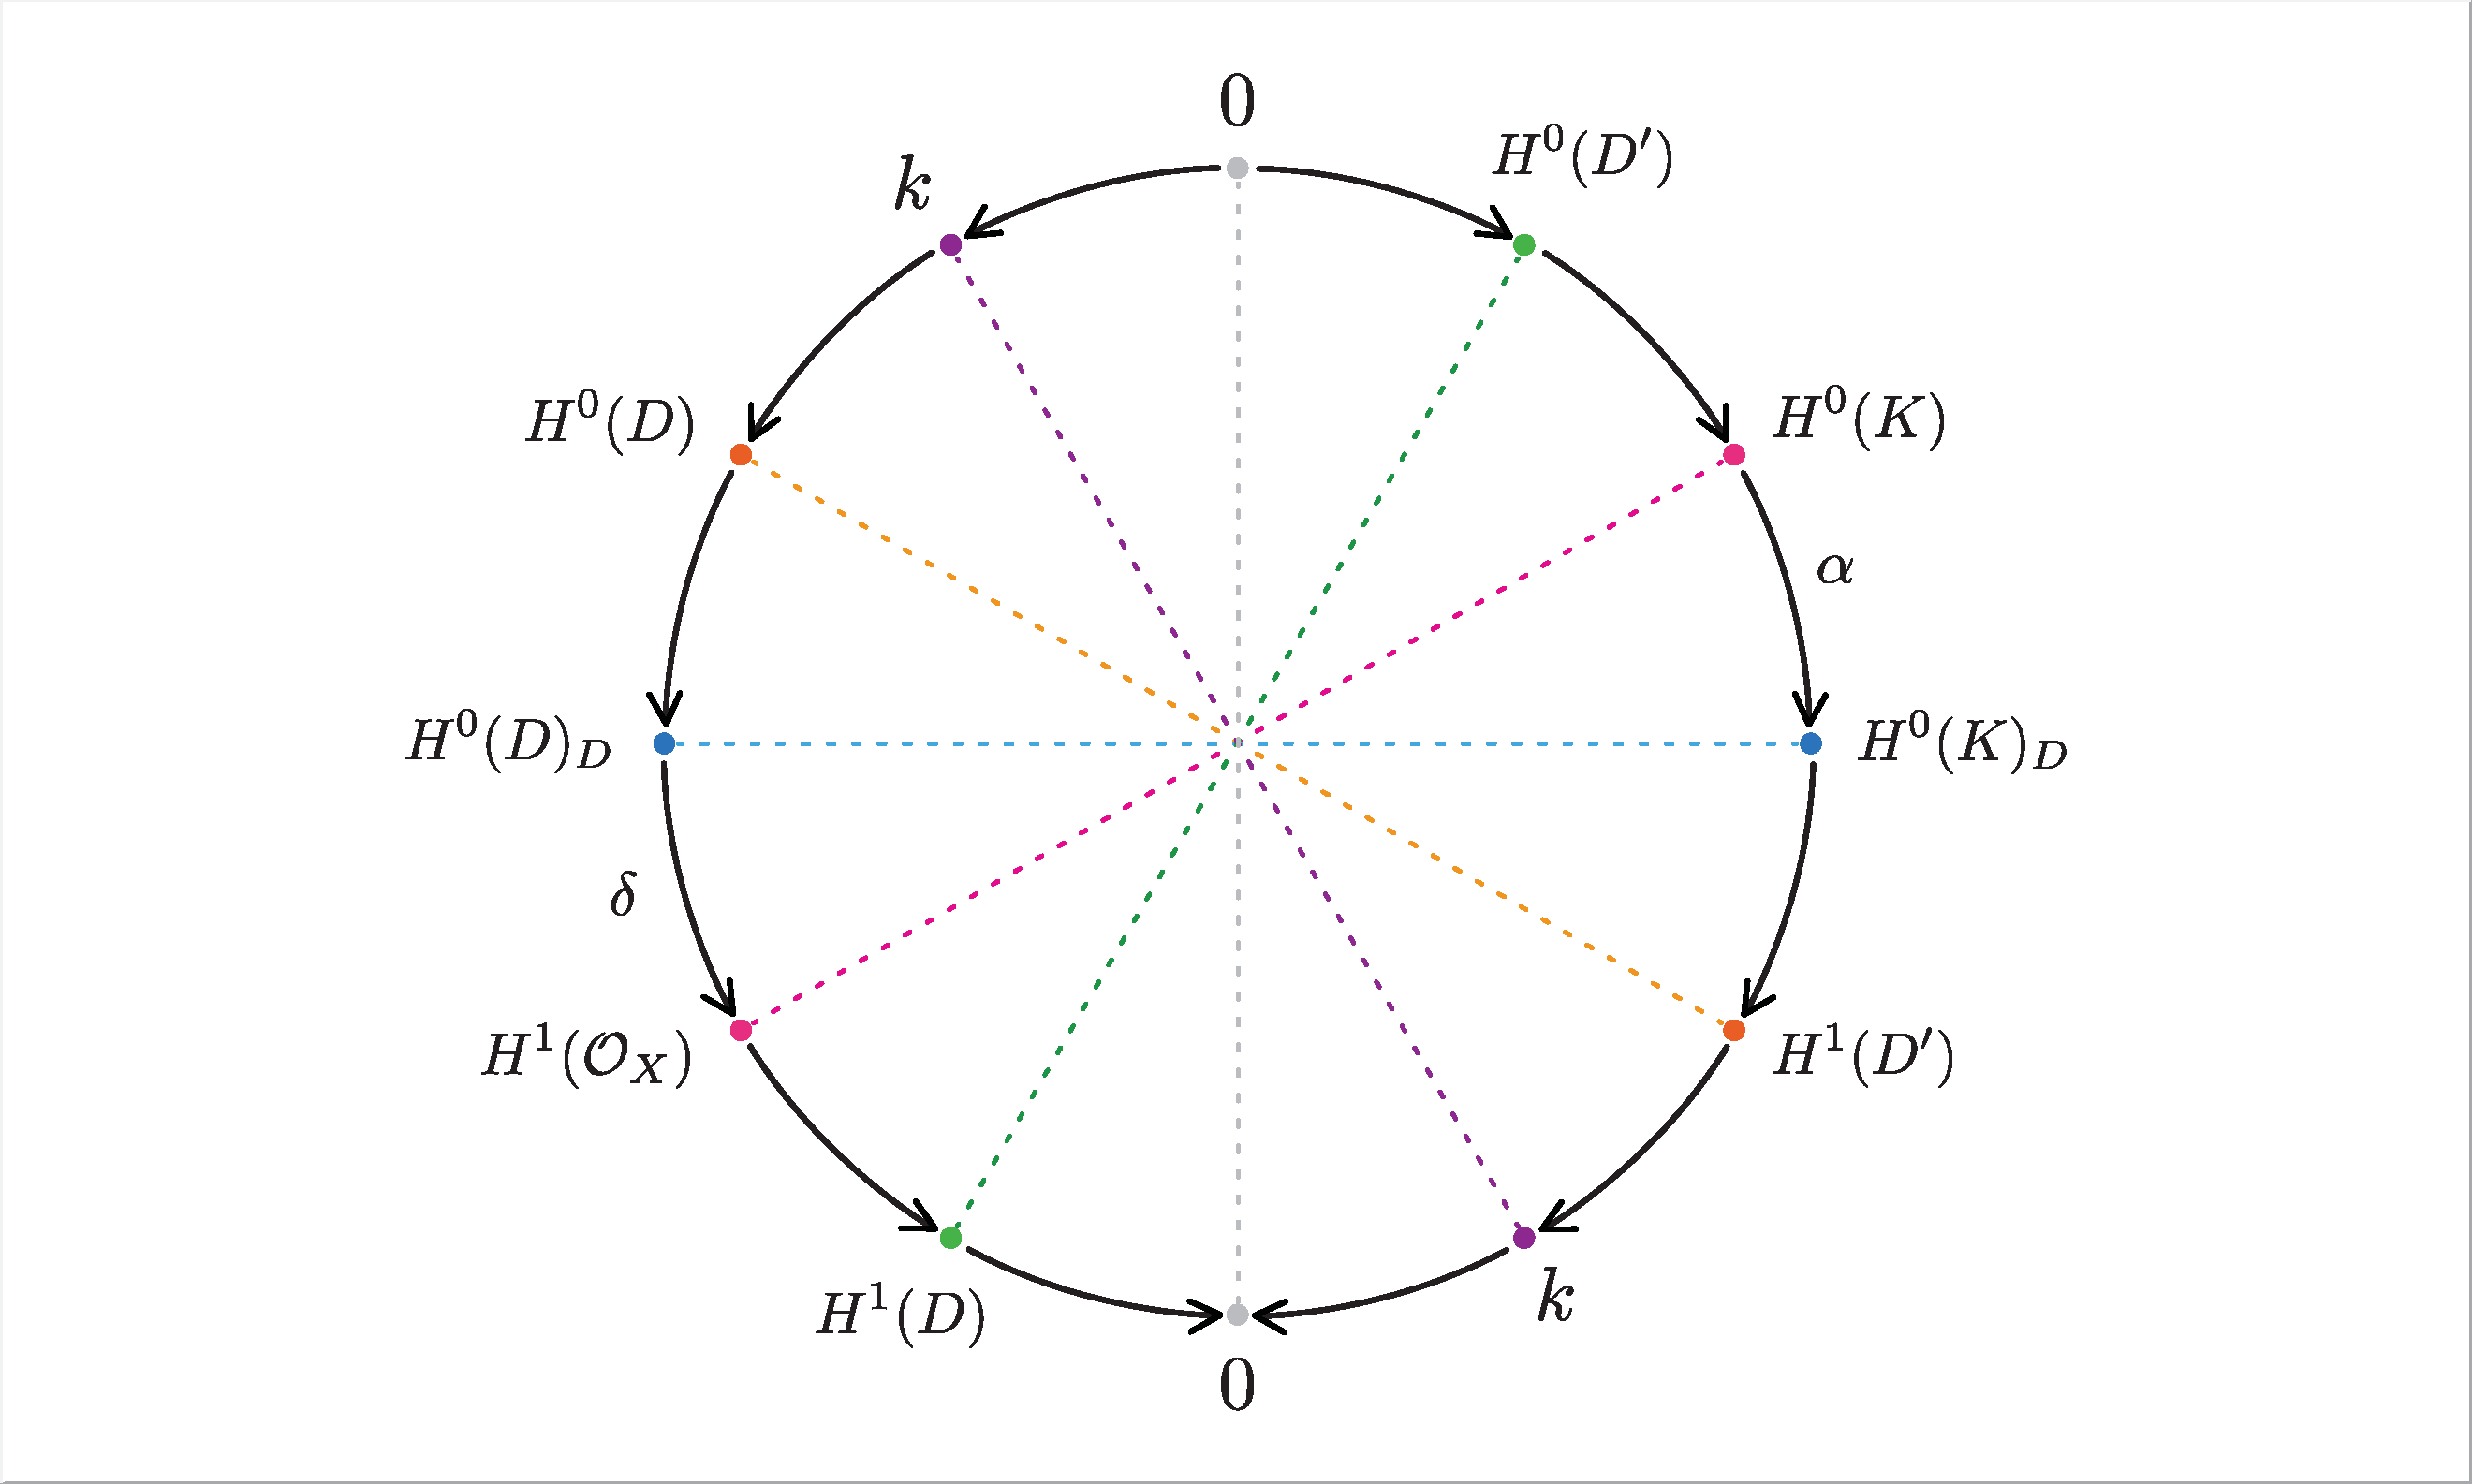
\includegraphics[width=0.9\textwidth]{Dual_Circle.pdf}
		\caption{ A more \emph{artistic} representation of the duality involved in diagram \eqref{eq:diagram} }
		\label{fig:Dual_Circle}
		\vspace{2em}
	\end{figure}


\section{Riemann-Roch Theorem}
	Using Serre duality we immediately get the final version of the theorem.
	\begin{namedtheo}[\RR Theorem]
		Let $X$ be a complete curve of genus $g$, $K$ a canonical divisor and $D\in \Dd$. Then
		\begin{equation}\label{thm:RR}
			h^0(D) - h^0(K-D) = d-g+1
		\end{equation}
	\end{namedtheo}
	Notice that, plugging-in the canonical class $K$ in the \RR formula and recalling that by definition $h^0(K) = g$, we get
	$$ \deg(K) = 2g-2 $$
	which, since $K$ is the dual of the tangent bundle, is an analogue of the Hopf index theorem for Riemann surfaces.
	
	
	
	
	
	
	
	% ---------------------------------------------------------------------------
	% ----------------------- end of thesis sub-document ------------------------


 %Appendix B - Riemann Roch & Serre Duality


%\include{7/discussion}               % discussion of results

%\include{8/materials_methods}        % description of lab methods




% --------------------------------------------------------------
%:                  BACK MATTER: appendices, refs,..
% --------------------------------------------------------------

% the back matter: appendix and references close the thesis


%: ----------------------- bibliography ------------------------

% The section below defines how references are listed and formatted
% The default below is 2 columns, small font, complete author names.
% Entries are also linked back to the page number in the text and to external URL if provided in the BibTex file.

% PhDbiblio-url2 = names small caps, title bold & hyperlinked, link to page 
%\begin{multicols}{2} % \begin{multicols}{ # columns}[ header text][ space]
  
\begin{small} % tiny(5) < scriptsize(7) < footnotesize(8) < small (9)

  \bibliographystyle{Latex/Classes/PhDbiblio-url2} % Title is link if provided
  \renewcommand{\bibname}{Bibliography} % changes the header; default: Bibliography

  \bibliography{9_backmatter/bibliografia} % adjust this to fit your BibTex file

\end{small}


%\end{multicols}

% --------------------------------------------------------------
% Various bibliography styles exit. Replace above style as desired.

% in-text refs: (1) (1; 2)
% ref list: alphabetical; author(s) in small caps; initials last name; page(s)
%\bibliographystyle{Latex/Classes/PhDbiblio-case} % title forced lower case
%\bibliographystyle{Latex/Classes/PhDbiblio-bold} % title as in bibtex but bold
%\bibliographystyle{Latex/Classes/PhDbiblio-url} % bold + www link if provided

%\bibliographystyle{Latex/Classes/jmb} % calls style file jmb.bst
% in-text refs: author (year) without brackets
% ref list: alphabetical; author(s) in normal font; last name, initials; page(s)

%\bibliographystyle{plainnat} % calls style file plainnat.bst
% in-text refs: author (year) without brackets
% (this works with package natbib)


% --------------------------------------------------------------

% according to Dresden med fac summary has to be at the end
%
% Thesis Abstract -----------------------------------------------------


%\begin{abstractslong}    %uncommenting this line, gives a different abstract heading
\begin{abstracts}         %this creates the heading for the abstract page

	We give an overview of the foundations and the basic results of the classical \BN Theory, dealing with the geometry of the moduli varieties parametrizing effective divisors and linear series on a given curve.\\
	We mainly follow the treatment proposed in the book \emph{Geometry of Algebraic Curves} written by Arbarello, Cornalba, Griffiths and Harris. 
	The classical theory, as presented in the book, was developed during the last century for curves over the complex numbers.\\ 
	Our discussion, instead, avoids the use of any complex-analytic tool and it is completely formulated in terms of modern algebraic geometry. As a result of this more general approach, we are able to generalize two key results of the classical theory -- the Existence and Connectedness Theorems -- to curves over an arbitrary algebraically closed field.\\
	It is important to highlight that the \BN theory heavily relies on homological algebra and, in particular, a crucial role is played by the so called Petri's map, which is in fact a cohomolgical cup-product homomorphism. Hence it seems reasonable to guess that the concepts described in the classical theory are not strictly dependent on complex analysis and, thus, that most of its results can be extended to more general fields.
	\vspace{12em}
	\begin{center}
		\footnotesize{
			The complete LaTex source of this document can be downloaded from the repository \\ 
			\href{https://github.com/AndreaBarbon/Algebraic-Brill-Noether-Theory}{https://github.com/AndreaBarbon/Algebraic-Brill-Noether-Theory}
		}
	\end{center}

\end{abstracts}
%\end{abstractlongs}


% ---------------------------------------------------------------------- 


%: Declaration of originality
%\include{9_backmatter/declaration}



\end{document}
